\documentclass[12pt, a4paper]{article}
\usepackage[utf8]{inputenc}
\usepackage{graphicx}
\usepackage{hyperref}
\usepackage{apacite}
\usepackage{float}
\let\cite\shortcite
\usepackage{setspace}
\usepackage{subfig}
\usepackage{multirow}
\usepackage{rotating}
\usepackage{tablefootnote}
\usepackage{dcolumn}
\usepackage{caption}
\usepackage{amsmath}

\usepackage{enumitem,booktabs,cfr-lm}
\makeatother

\spacing{1}
\usepackage[table,xcdraw]{xcolor} 
\usepackage{pgf}
\usepackage{pgfplots} 
\pgfplotsset{compat=newest}
\pgfplotsset{plot coordinates/math parser=false}
\usepackage{pdfpages}

\bibliographystyle{apacite}
\usepackage[a4paper]{geometry}
\geometry{top=2.54 cm, bottom=2.54 cm, left=2.54 cm, right=2.54 cm}

\renewcommand*\contentsname{Índice}
\renewcommand{\figurename}{Figura}
\renewcommand{\tablename}{Tabla}
\renewcommand{\theenumi}{E\arabic{enumi}}
\renewcommand{\listfigurename}{Índice de Figuras}
\renewcommand{\listtablename}{Índice de Tablas}

\newcommand\nafootnote[1]{%
  \begingroup
  \renewcommand\thefootnote{}\footnote{\textit{n.a.} No aplica}%
  \endgroup
}
\begin{document}
\renewcommand{\refname}{Referencias}
\thispagestyle{empty}
			\begin{figure}[ht]
		   \minipage{\textwidth}
				\includegraphics[width=3cm]{Imagenes/acustica-color.png}
				\label{escudoTecNM}
		   \endminipage
		   \minipage{\textwidth}
				
\includegraphics[width=5cm]{Imagenes/UACh_Marcacolor.png}
				\label{EscudoITCJ}
			\endminipage
				%%\vspace{-1cm}
		\end{figure}
		
		\vspace{0.1cm}
		
		\begin{center}
		    {\scshape\LARGE \textbf{Universidad Austral de Chile} \par}
			{\scshape\Large Instituto de Acústica \par}
            \vspace{0.3cm}
             {\Large \textbf{Proyecto acústico - Acondicionamiento acústico ACUS$213$}}

			% Restauramos el interlineado:
			\begin{center}
				
			{\LARGE\bfseries ``Acondicionamiento acústico de salas de reuniones y sala de ensayo, Campus Los Canelos, UACh'' \par}
            \vspace{0.75cm}
            
		{\scshape\Large Fecha de entrega: $29$ de Noviembre de $2023$\par}	
        \vspace{0.75cm}
	    \LARGE	{ \textbf{Profesor:}}\\
        \large		{Felipe Figueroa}\\
        
		\vspace{0.5cm}	
		
		\LARGE	{ \textbf{Estudiante:}}\\
        \large	 {Daniela Narváez}\\
        \large   {Rafael Hayde}
    
        
        
        \normalsize	 {}

%% \it es letra itálica
				\vspace{1.25cm}
				\vspace{0.9cm}
				
			\end{center}
	
		\end{center}
\tableofcontents
\newpage
\section{Introducción}
El acondicionamiento acústico consiste en la definición de las formas y revestimientos 
de las superficies interiores de un recinto con objeto de conseguir las condiciones acústicas más 
adecuadas para el tipo de actividad a la que se haya previsto destinarlo.\cite{carrion1990diseno} \\
El presente informe tiene como objetivo analizar y proponer soluciones para el acondicionamiento acústico 
de dos salas de reuniones y una sala de ensayo de orquesta. \\
\noindent
La importancia del acondicionamiento acústico radica en su capacidad para mejorar la experiencia auditiva 
de las personas que utilizan estos espacios. En el caso de las salas de reuniones, es imprescindible una óptima 
inteligibilidad de la palabra ya que la comprensión del mensaje oral es de suma importancia. \cite{carrion1990diseno}
En el contexto de una sala de ensayo de orquesta, el acondicionamiento acústico es crucial para lograr una reproducción 
fiel y equilibrada de los instrumentos musicales, permitiendo a los músicos escucharse entre sí y trabajar en conjunto 
de manera óptima. \\
\noindent
Para llevar a cabo este proyecto, se utilizará normativas que indican el procedimiento de medición tiempo de reverberación y cálculo de parámetros acústicos como la ISO $3382-2$ \cite{ISO3382-2}.

\section{Objetivos}
\begin{itemize}
    \item \textbf{Objetivo General:} \\
    Proponer un acondicionamiento acústico para dos salas de reuniones y una sala de ensayo de orquesta, en el Centro de Extensión Campus los Canelos, UACh.

    \item \textbf{Objetivos Específicos:}
    \begin{itemize}
        \item Caracterizar acústicamente las salas.
        \item Analizar los parámetros acústicos de las salas.
        \item Generar una propuesta de diseño de acondicionamiento acústico para optimizar el sonido de las salas.
        \item Comparar los resultados mediante recomendaciones internacionales. 
        \item Elaborar un presupuesto del acondicionamiento acústico para cada sala.

    \end{itemize}
\end{itemize}
%\include{Contenido/2.Objetivos}
\section{Antecedentes del recinto}
\noindent 
El Centro de Extensión Campus Los Canelos de la Universidad Austral de Chile, ubicado en la calle Yerbas Buenas, en la ciudad de Valdivia, inaugurado en $2019$, busca ``acoger y congregar a diferentes comunidades en torno a las artes, las culturas, la extensión científica, temas públicos e iniciativas del área de la salud. Atendiendo a los lineamientos y políticas de vinculación con el medio universitarias se priorizó la adecuación de los espacios con una orientación hacia su uso público. Este centro cuenta con tres salones multiuso para exposiciones, charlas y conferencias, sumando más de $250$ $m^2$ de superficie totalmente equipados con sistemas de audio y video. Además, alberga a las distintas unidades, programas y áreas que conforman la Dirección de Vinculación con el medio, con un espacio cercano a los $300$ $m^2$ utilizados como salas de reuniones y oficinas.'' \cite{loscanelos}

\begin{figure}[H]
    \centering
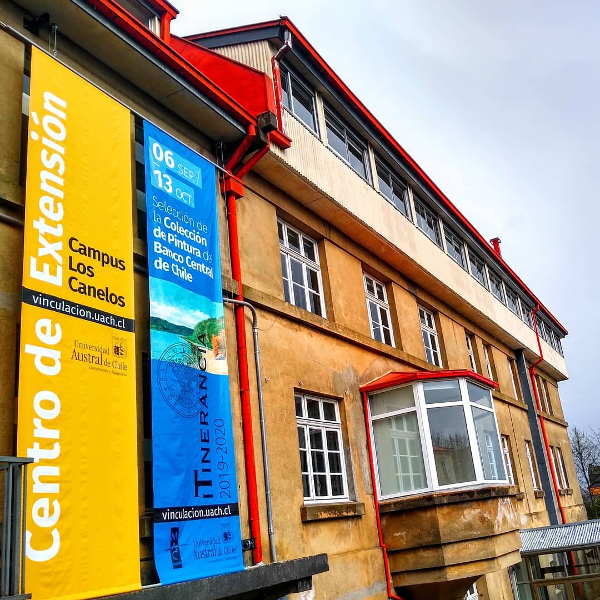
\includegraphics[scale=0.45]{Imagenes/centroextensionuach.jpg}
    \caption{Centro de Extensión Campus los Canelos, UACh.}
    \label{fig:los-canelos}
\end{figure}

\noindent En específico, este proyecto considera el acondicionamiento acústico de dos salas de reuniones, de $30$ y $35$ $m^2$, y la sala de ensayo de la Orquesta de Cámara de Valdivia, de $62$ $m^2$.

\noindent El Centro de Extensión Campus Los Canelos de la Universidad Austral de Chile, como se puede observar en la figura \ref{fig:geolocalización} se encuentra ubicado en Yerbas Buenas $181$, en la ciudad de Valdivia.
\begin{figure}[H]
    \centering
    \includegraphics[scale=0.5]{Imagenes/Antecedentes/Geolocalización.png}
    \caption{Geolocalización del edificio}
    \label{fig:geolocalización}
\end{figure}

\noindent Los salones a estudiar dentro del recinto son dos salas de reuniones con soporte para videoconferencia y una sala de ensayo utilizada por la Orquesta de Cámara de Valdivia, como se puede observar en las Figuras \ref{fig: foto sala1}, \ref{fig: foto sala2} y \ref{fig: foto sala OCV} respectivamente.
\begin{figure}[H]
    \centering
    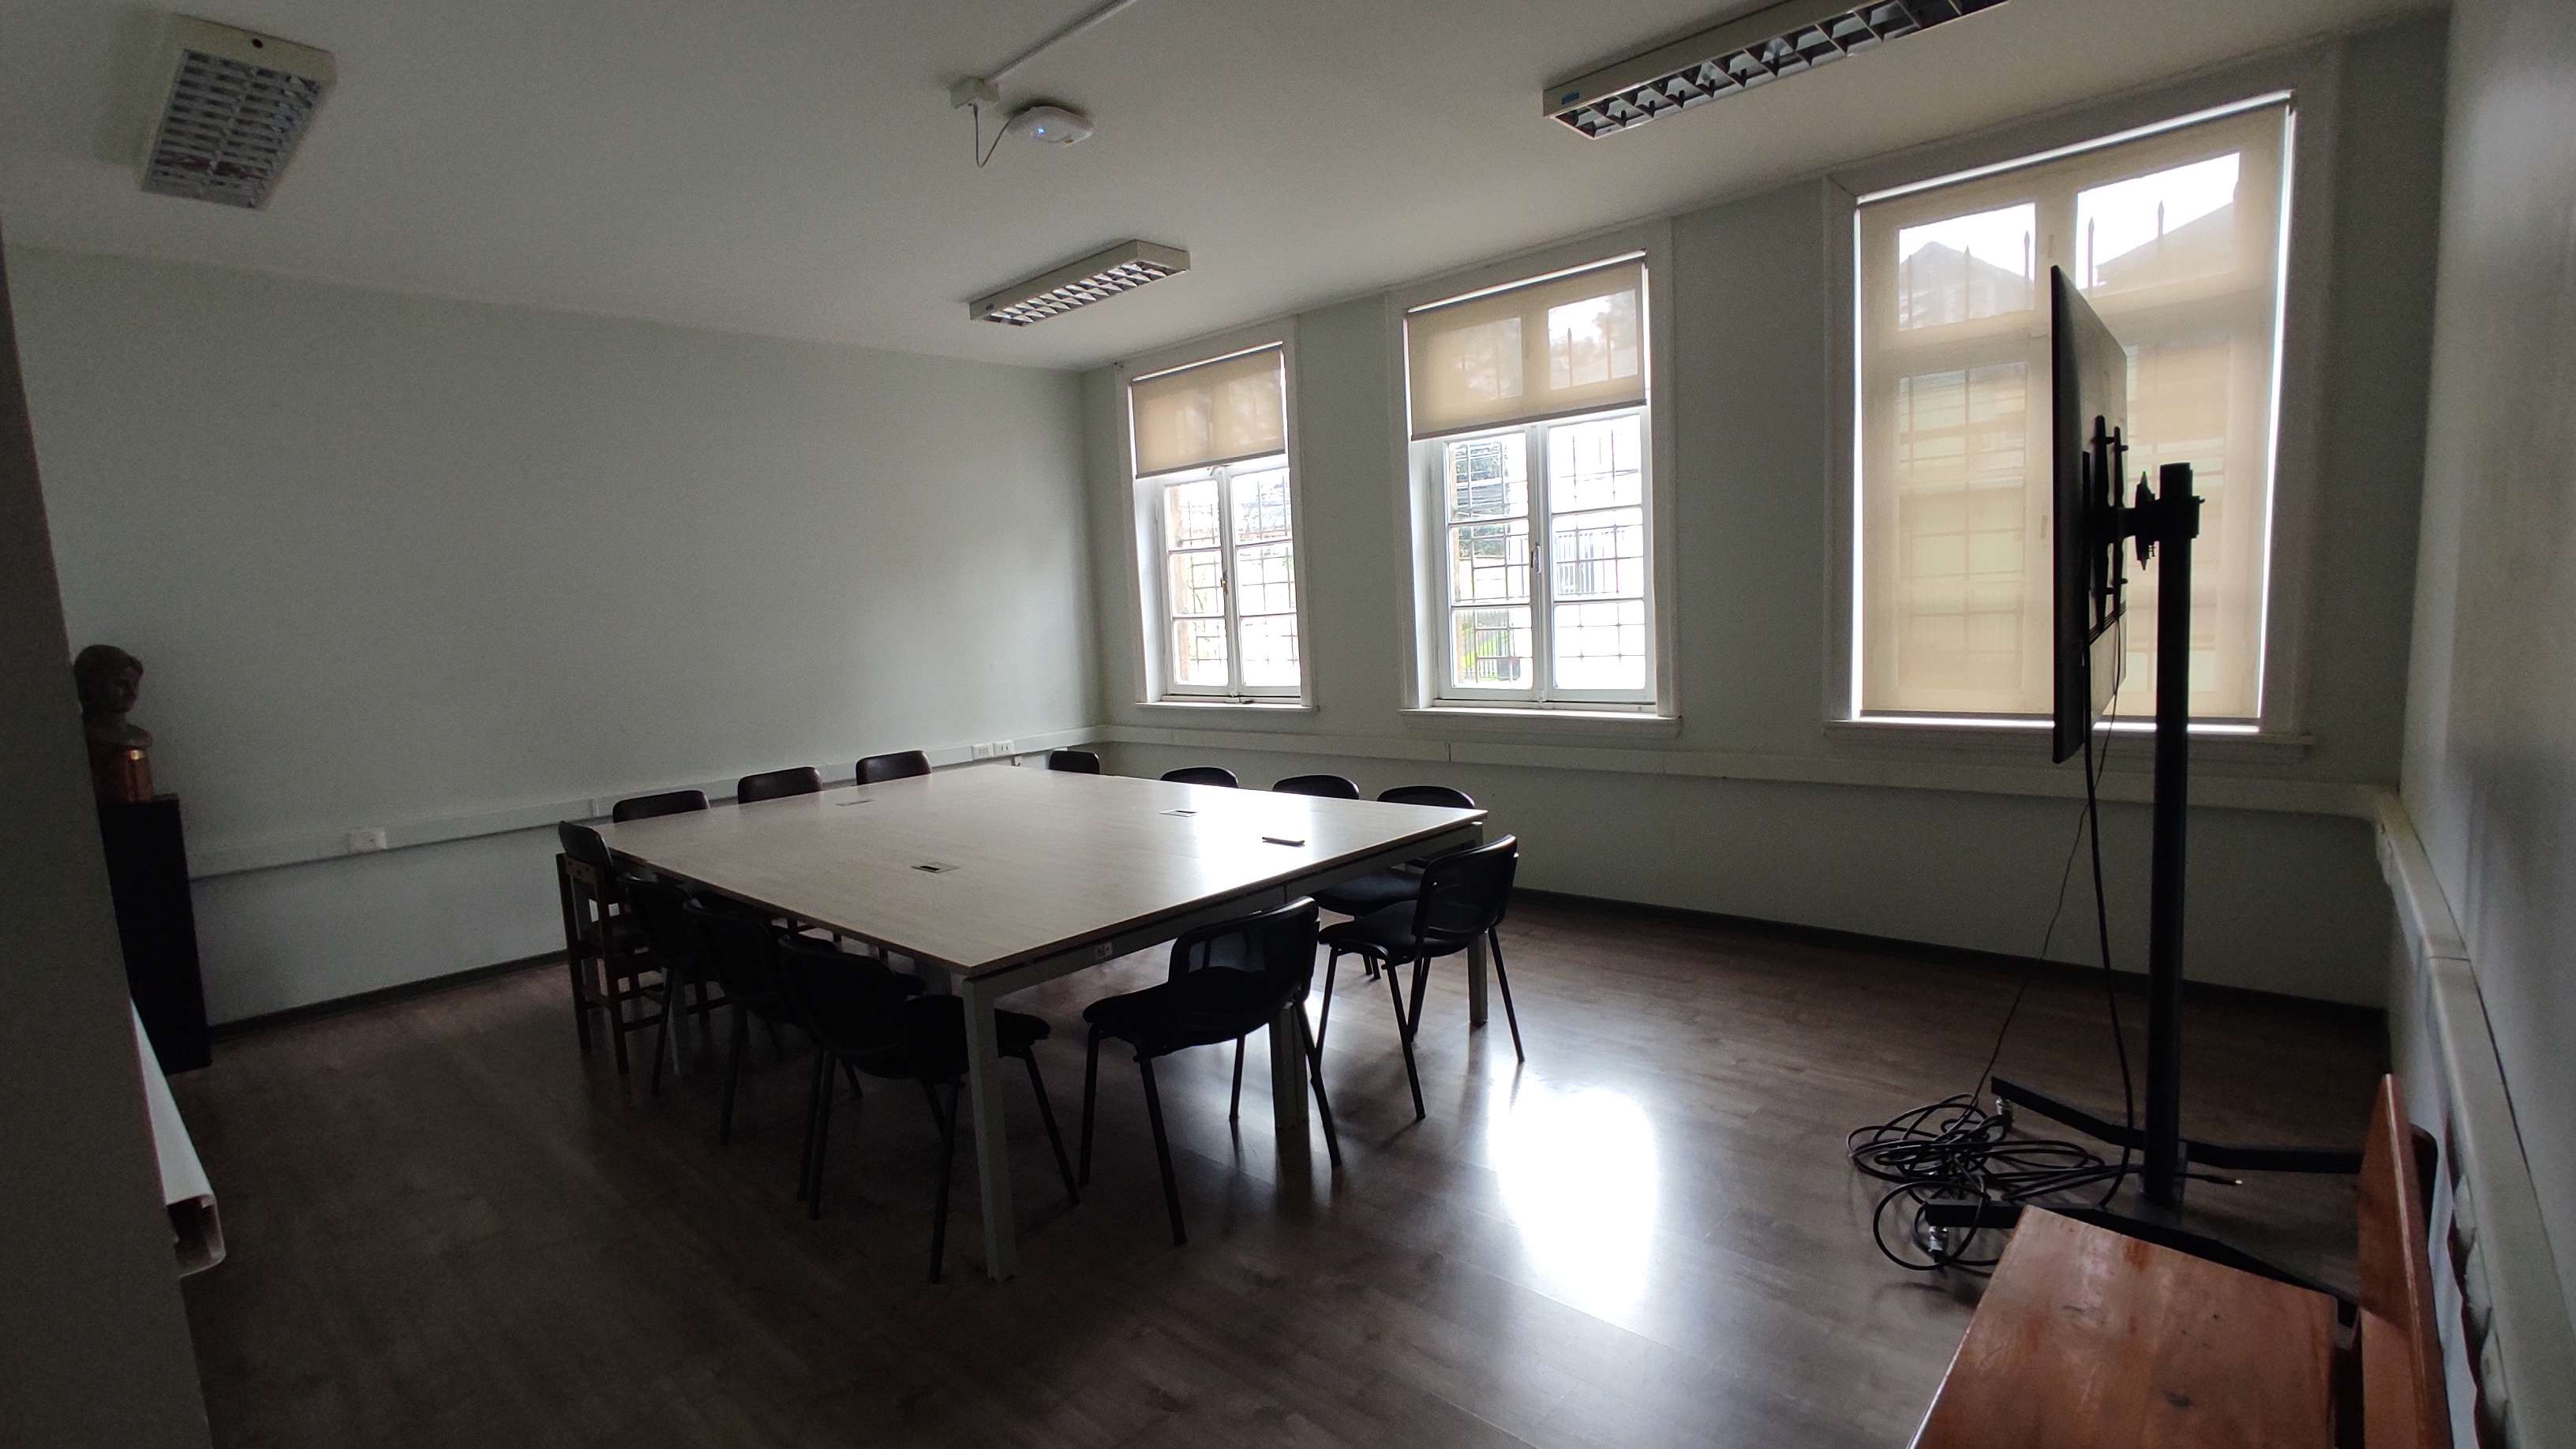
\includegraphics[scale=0.1]{Imagenes/Antecedentes/Sala 1.jpg}
    \caption{Fotografía de sala de reunión 1}
    \label{fig: foto sala1}
\end{figure}

\begin{figure}[H]
    \centering
    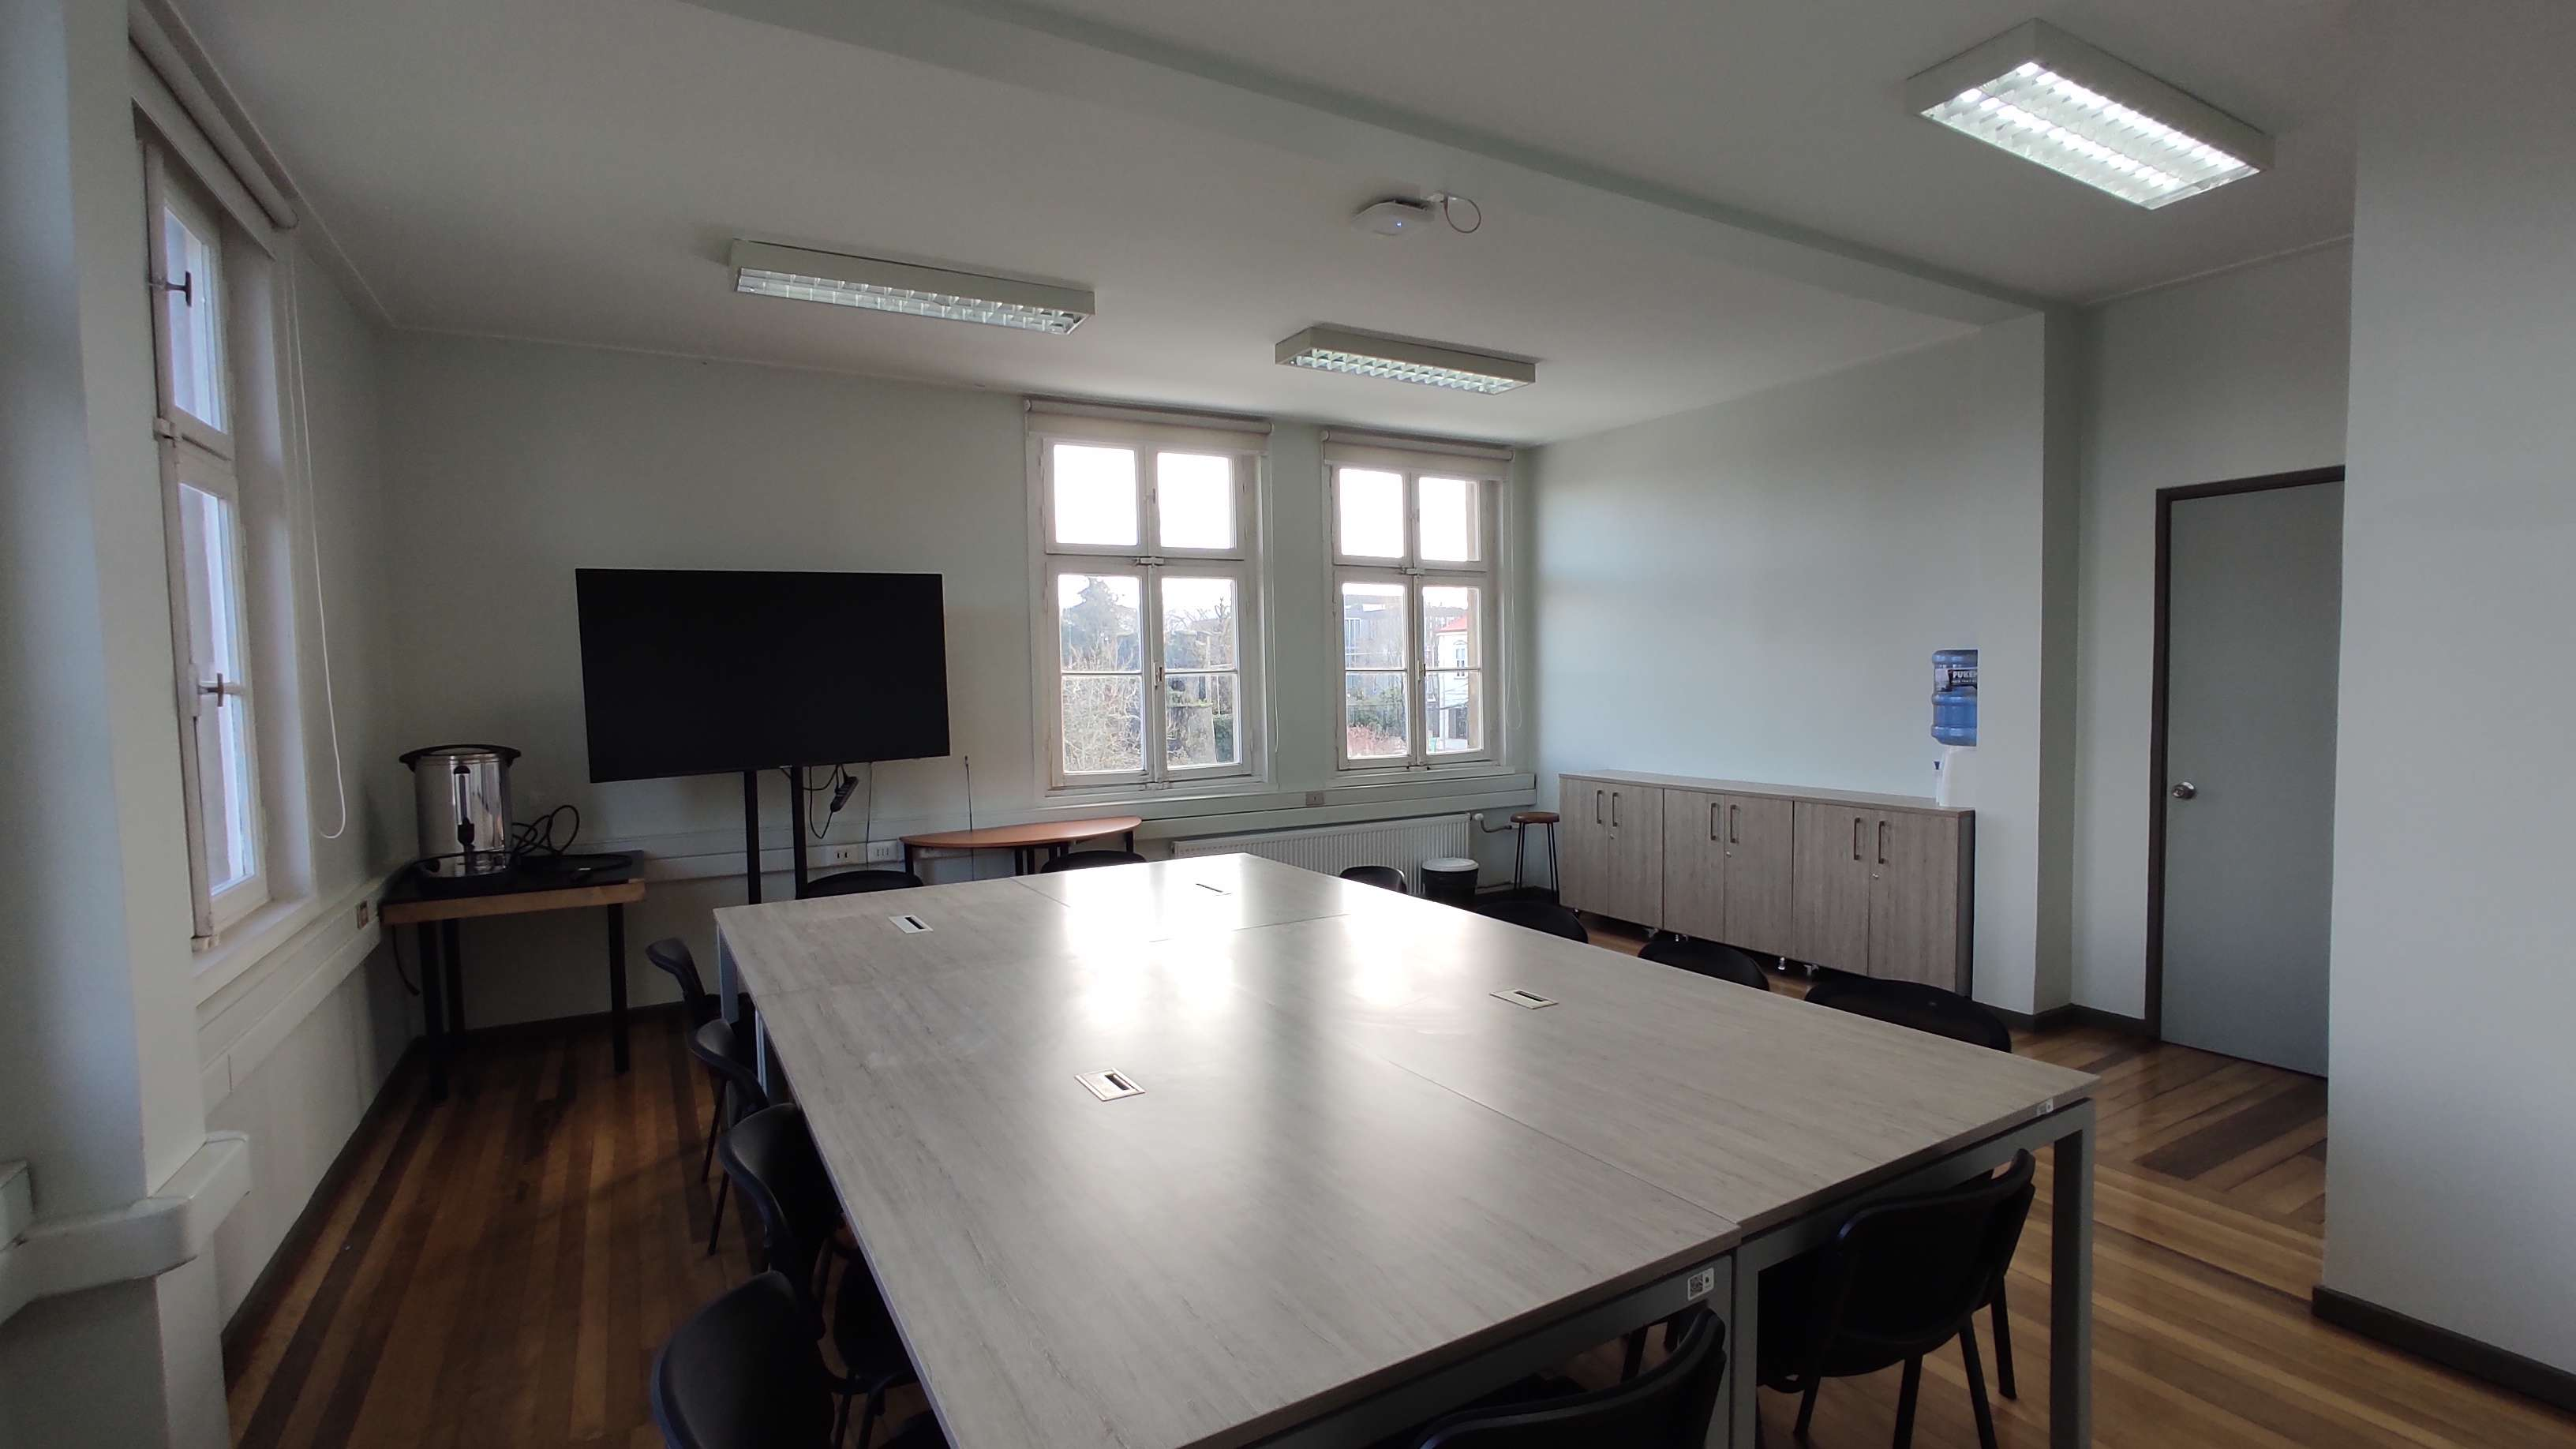
\includegraphics[scale=0.1]{Imagenes/Antecedentes/Sala 2.jpg}
    \caption{Fotografía de sala de reunión 2}
    \label{fig: foto sala2}
\end{figure}

\begin{figure}[H]
    \centering
    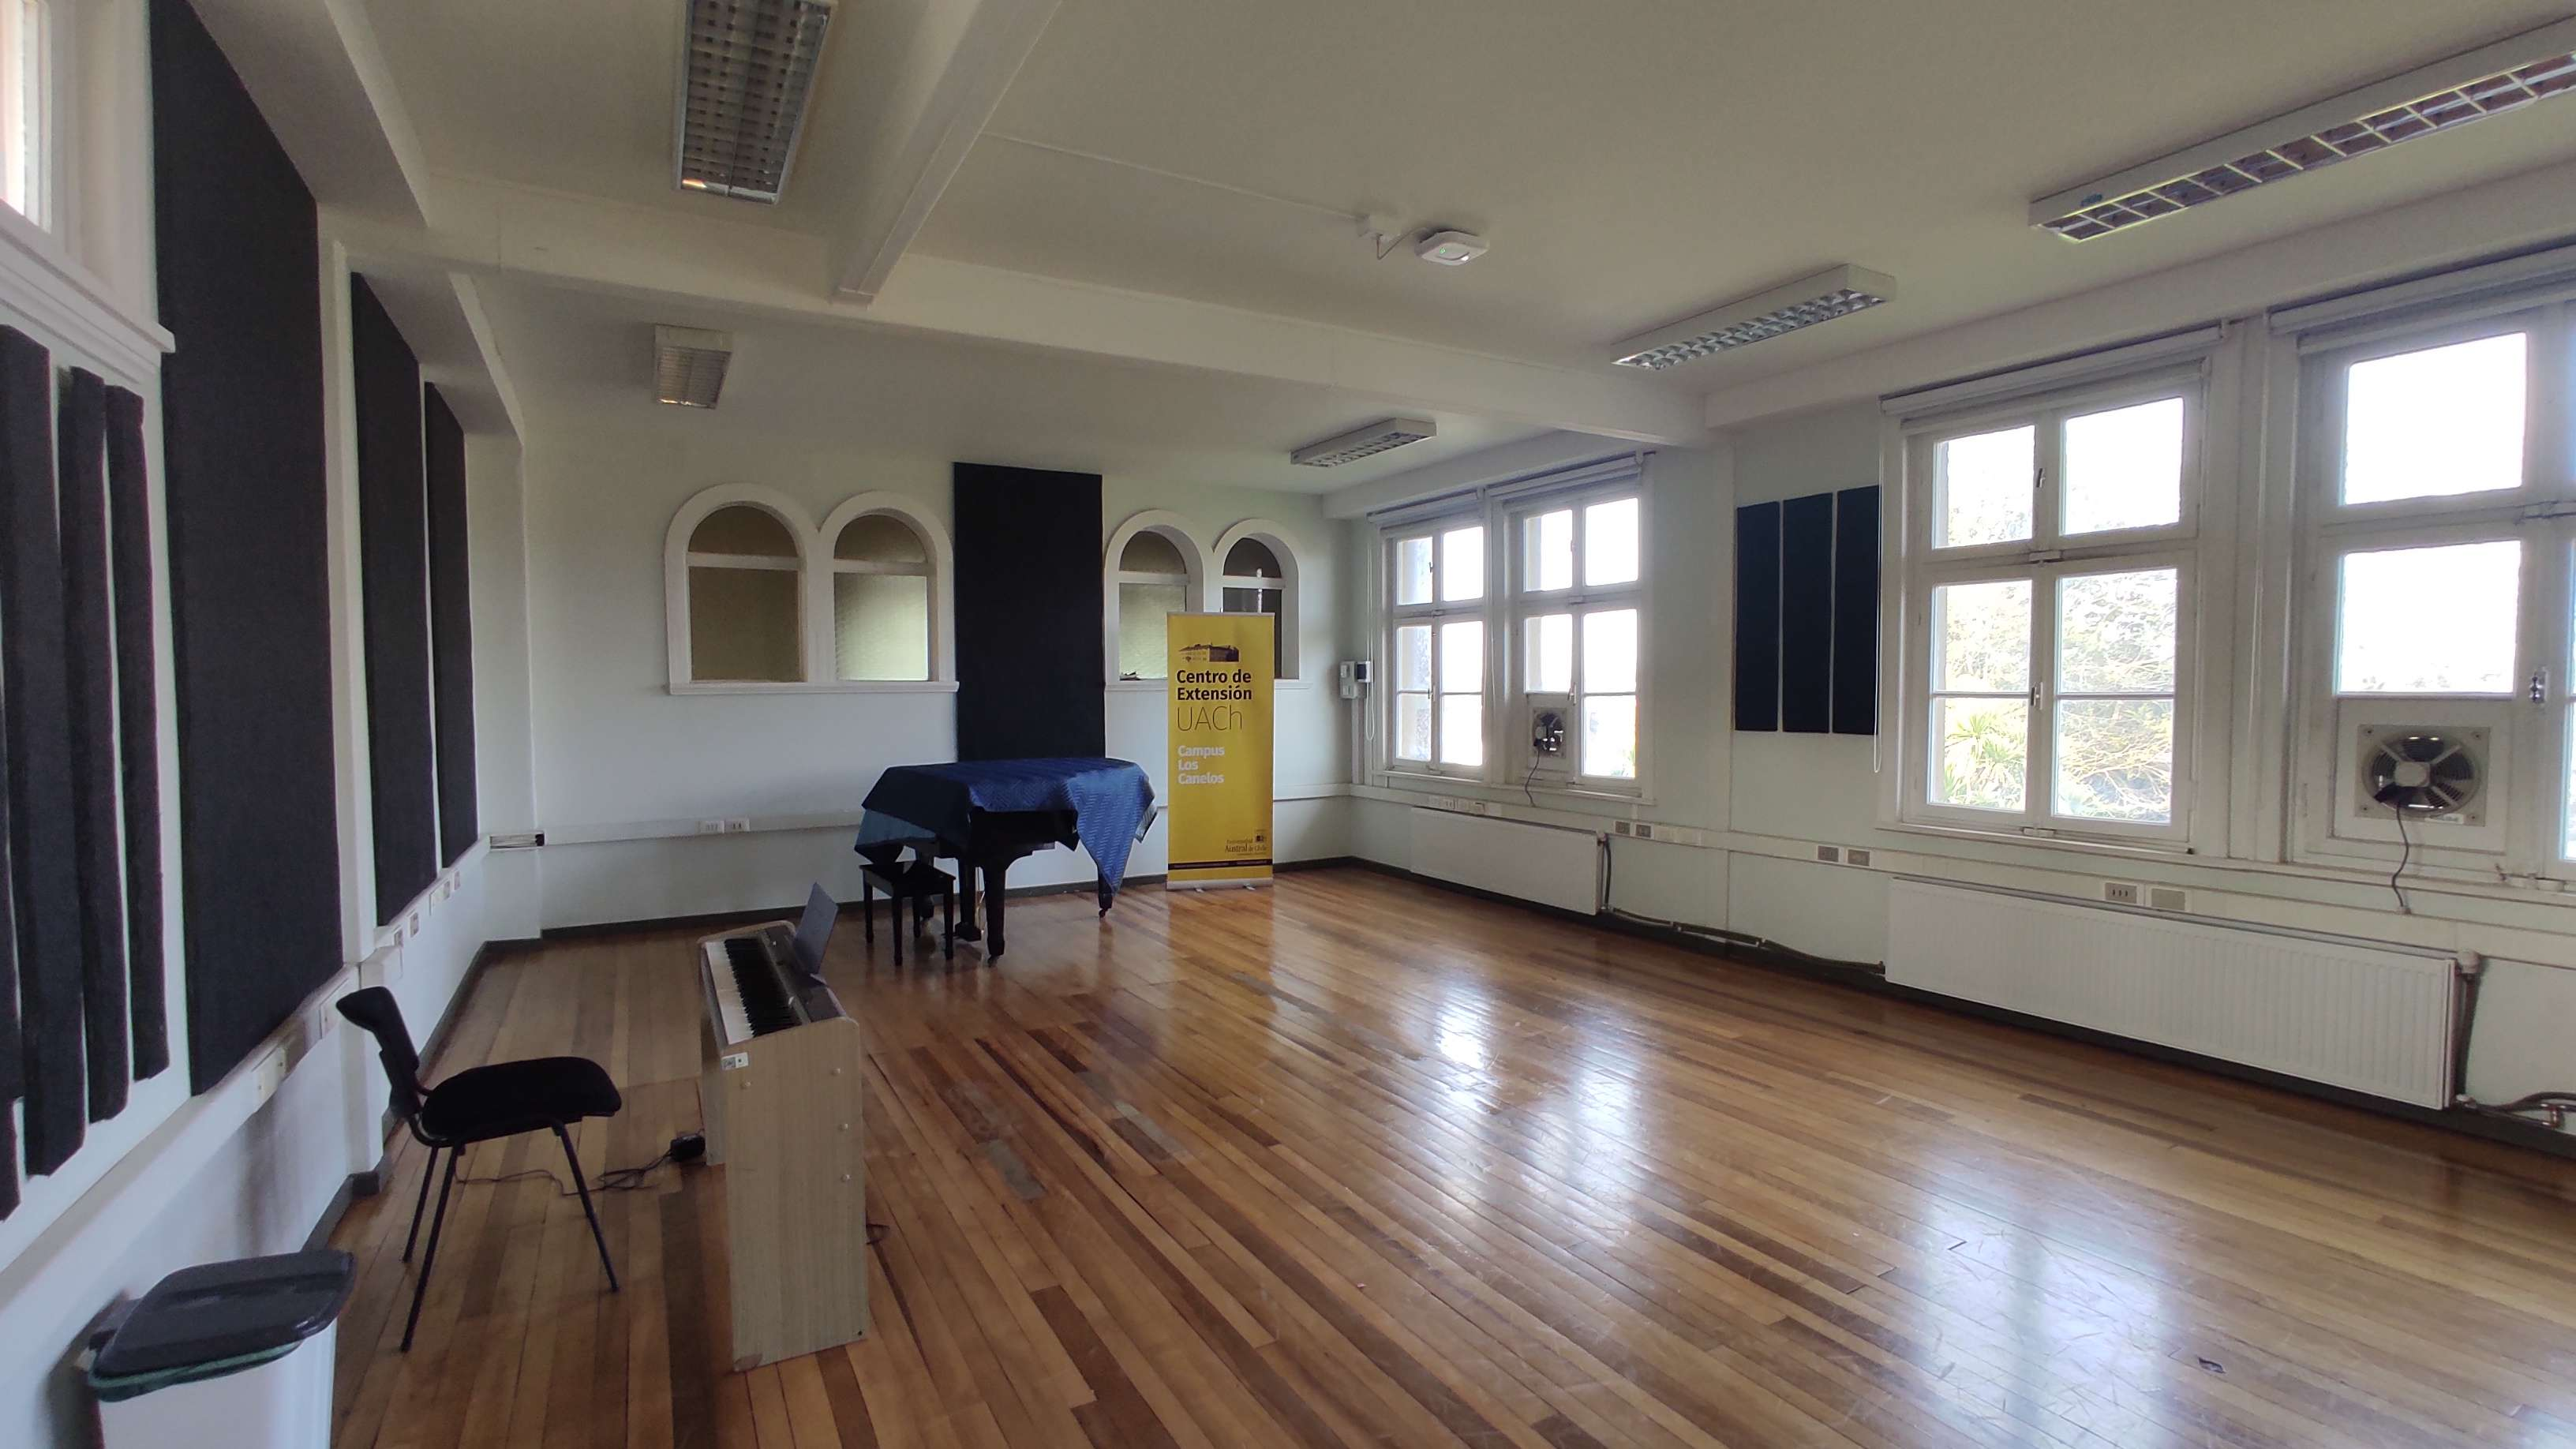
\includegraphics[scale=0.1]{Imagenes/Antecedentes/Sala OCV.jpg}
    \caption{Fotografía de sala de ensayo}
    \label{fig: foto sala OCV}
\end{figure}

\section{Planificación}
\subsection{Plan de trabajo}
Para elaborar el proyecto es importante la realización de actividades las cuales se ven descritas en la tabla \ref{tab: plan de trabajo} con sus respectivos resultados esperados para un trabajo óptimo.
\begin{table}[H]
\centering
\caption{Plan de trabajo}
\label{tab: plan de trabajo}
\resizebox{\textwidth}{!}{%
\begin{tabular}{|c|l|l|l|}
\hline
\textbf{Actividad}    & \multicolumn{1}{c|}{\textbf{Descripción}}                                                                                                             & \multicolumn{1}{c|}{\textbf{Resultado esperado}}                                                                                                         & \multicolumn{1}{c|}{\textbf{Indicador de cumplimiento}}                                                                                        \\ \hline
Planificación         & \begin{tabular}[c]{@{}l@{}}Establecer contacto con el \\ establecimiento y \\ planificación de actividades\end{tabular}                               & Organización del proyecto                                                                                                                                & Carta Gantt y puntos de medición                                                                                                               \\ \hline
Mediciones            & \begin{tabular}[c]{@{}l@{}}Realizar mediciones de \\ dimensión, ruido de fondo \\ y tiempo de reverberación \\ de las salas\end{tabular}              & \begin{tabular}[c]{@{}l@{}}Mediciones de respuesta al \\ impulso de las salas, \\ geometría y volumen\end{tabular}                                       & \begin{tabular}[c]{@{}l@{}}Datos de características físicas y \\ acústicas del recinto\end{tabular}                                            \\ \hline
Modelación            & \begin{tabular}[c]{@{}l@{}}Modelar las salas en \\ software CAD\end{tabular}                                                                          & \begin{tabular}[c]{@{}l@{}}Modelo en software EASE\\  del recinto\end{tabular}                                                                           & \begin{tabular}[c]{@{}l@{}}Archivo de software EASE con \\ modelo del recinto\end{tabular}                                                     \\ \hline
Análisis de datos     & \begin{tabular}[c]{@{}l@{}}Procesar y tabular los datos\\ obtenidos de las mediciones\end{tabular}                                                    & \begin{tabular}[c]{@{}l@{}}Tabla comparativa con \\ recomendaciones\end{tabular}                                                                         & \begin{tabular}[c]{@{}l@{}}Archivo CSV con los datos \\ procesados de las mediciones\end{tabular}                                              \\ \hline
Diseño de propuesta   & \begin{tabular}[c]{@{}l@{}}Proponer un diseño de \\ acondicionamiento acústico \\ acorde con recomendaciones \\ para las salas\end{tabular}           & \begin{tabular}[c]{@{}l@{}}Determinar una solución de\\  acondicionamiento acústico\\ óptimo para los usos de las \\ salas\end{tabular}                  & \begin{tabular}[c]{@{}l@{}}Documentación del detalle y \\ archivo de software EASE con la \\ implementación de la propuesta\end{tabular}       \\ \hline
Análisis de propuesta & \begin{tabular}[c]{@{}l@{}}Evaluar el acondicionamiento \\ acústico a través \\ de software EASE\end{tabular}                                         & \begin{tabular}[c]{@{}l@{}}Comprobar el mejoramiento \\ de las características acústicas\\ de cada sala\end{tabular}                                     & \begin{tabular}[c]{@{}l@{}}Tabla comparativa de los parámetros \\ de las salas acondicionadas y \\ recomendaciones bibliográficas\end{tabular} \\ \hline
Presupuesto de diseño & \begin{tabular}[c]{@{}l@{}}Presentar una cotización de \\ los elementos y materiales\\  propuestos para el \\ acondicionamiento acústico\end{tabular} & \begin{tabular}[c]{@{}l@{}}Listado de los elementos \\ requeridos para el \\ acondicionamiento en el\\ mercado y sus respectivos \\ valores\end{tabular} & \begin{tabular}[c]{@{}l@{}}Presupuesto de los elementos que \\ componen la propuesta de \\ acondicionamiento acústico\end{tabular}             \\ \hline
Redacción de informe  & \begin{tabular}[c]{@{}l@{}}Evidenciar el desarrollo del \\ proyecto mediante avances \\ progresivos\end{tabular}                                      & \begin{tabular}[c]{@{}l@{}}Plasmar los resultados del \\ trabajo realizado en el \\ proyecto\end{tabular}                                                & Informe final del proyecto                                                                                                                     \\ \hline
Elaboración de póster & \begin{tabular}[c]{@{}l@{}}Sintetizar la información \\ presente en el informe en \\ formato póster\end{tabular}                                      & Resumen general del proyecto                                                                                                                             & Póster                                                                                                                                         \\ \hline
\end{tabular}%
}
\end{table}


\newpage

\subsection{Cronograma}
\noindent A continuación, en la tabla \ref{tab: carta gantt} se puede observar la planificación respectiva del proyecto, partir de las actividades planteadas en la tabla \ref{tab: plan de trabajo}. Esta planificación se plantea por semanas, desde la semana del $21$ de agosto hasta la semana del $2$ de diciembre del presente año. Los números señalan la cantidad de horas que se emplearan en realizar cada actividad. Las semanas destacadas son las que corresponden a las entregas de avances del proyecto.
\begin{table}[H]
\centering
\caption{Carta Gantt del proyecto}
\label{tab: carta gantt}
\resizebox{16cm}{!} {
\begin{tabular}{|l|llllllllllllllll|}
\hline
 & \multicolumn{16}{c|}{Semanas} \\ \cline{2-17} 
\multirow{-2}{*}{Actividad} & $1$ & \cellcolor[HTML]{FABF8F}$2$ & $3$ & {\cellcolor[HTML]{FABF8F}$4$} & $5$ & $6$ & $7$ & {\cellcolor[HTML]{FABF8F}$8$} & $9$ & $10$ & \cellcolor[HTML]{FABF8F}$11$ & \multicolumn{1}{|l|}{$12$} & $13$ & $14$ & \cellcolor[HTML]{FABF8F}$15$ & \cellcolor[HTML]{FABF8F}$16$ \\ \hline
Planificación & \cellcolor[HTML]{4F81BD}$3$ & \cellcolor[HTML]{4F81BD}$4$ &  &  &  &  &  &  &  &  &  & \multicolumn{1}{|l|}{} &  &  &  &  \\
Mediciones &  & \cellcolor[HTML]{4F81BD}$6$ & {\cellcolor[HTML]{4F81BD}$3$} &  &  &  &  &  &  &  &  & \multicolumn{1}{|l|}{} &  &  &  &  \\
Modelación &  &  & {\cellcolor[HTML]{4F81BD}$6$} & {\cellcolor[HTML]{4F81BD}$6$} & \cellcolor[HTML]{4F81BD}$6$ &  &  &  &  &  &  & \multicolumn{1}{|l|}{} &  &  &  &  \\
Analisis de datos &  &  &  & {\cellcolor[HTML]{C0504D}$2$} & \cellcolor[HTML]{C0504D}$4$ &  &  &   &  &  &  & \multicolumn{1}{|l|}{} &  &  &  &  \\
Diseño de propuesta &  &  &  &  & \cellcolor[HTML]{C0504D}$4$ & \cellcolor[HTML]{C0504D}$4$ & \cellcolor[HTML]{C0504D}$4$ & {\cellcolor[HTML]{C0504D}$4$} & \cellcolor[HTML]{C0504D}$4$ & \cellcolor[HTML]{C0504D}$4$ &  & \multicolumn{1}{|l|}{} &  &  &  &  \\
Analisis de propuesta &  &  &  &  & \cellcolor[HTML]{C0504D}$2$ & \cellcolor[HTML]{C0504D}$2$ & \cellcolor[HTML]{C0504D}$2$ & {\cellcolor[HTML]{C0504D}$2$} & \cellcolor[HTML]{C0504D}$2$ & \cellcolor[HTML]{C0504D}$2$ &  & \multicolumn{1}{|l|}{} &  &  &  &  \\
Presupuesto de diseño &  &  &  &  &  &  &  &   & \cellcolor[HTML]{C0504D}$2$ & \cellcolor[HTML]{C0504D}$2$ & \cellcolor[HTML]{C0504D}$2$ & \multicolumn{1}{|l|}{\cellcolor[HTML]{C0504D}$2$} &  &  &  &  \\
Redacción de informe & \cellcolor[HTML]{9BBB59}$2$ & \cellcolor[HTML]{9BBB59}$2$ & {\cellcolor[HTML]{9BBB59}$2$} & {\cellcolor[HTML]{9BBB59}$2$} &  & \cellcolor[HTML]{9BBB59}$2$ & {\cellcolor[HTML]{9BBB59}$2$} & {\cellcolor[HTML]{9BBB59}$2$} &  & \cellcolor[HTML]{9BBB59}
$2$ & \cellcolor[HTML]{9BBB59}$2$ & \multicolumn{1}{|l|}{\cellcolor[HTML]{9BBB59}$2$} & {\cellcolor[HTML]{9BBB59}$2$} & \cellcolor[HTML]{9BBB59}$2$ & \cellcolor[HTML]{9BBB59}$2$ &  \\
Elaboración de poster &  &  &  &  &  &  &  &  &  &  &  & \multicolumn{1}{|l|}{} &  &  & \cellcolor[HTML]{538DD5}$2$ & \cellcolor[HTML]{538DD5}$2$ \\ \hline
\end{tabular}%
}
\end{table}
\noindent Actualmente el proyecto se encuentra en la semana $2$, en la cual se comienzan las mediciones.
\section{Metodología}
\subsection{Medición de dimensiones del recinto}
\noindent Para caracterizar el recinto, es necesario tener las dimensiones de cada sala. Parte del detalle de las dimensiones fueron proporcionadas por el encargado del Campus Los Canelos. En la figura \ref{fig: planos CAD} se puede observar una vista superior de las salas a estudiar.

\begin{figure}[H]
    \centering
    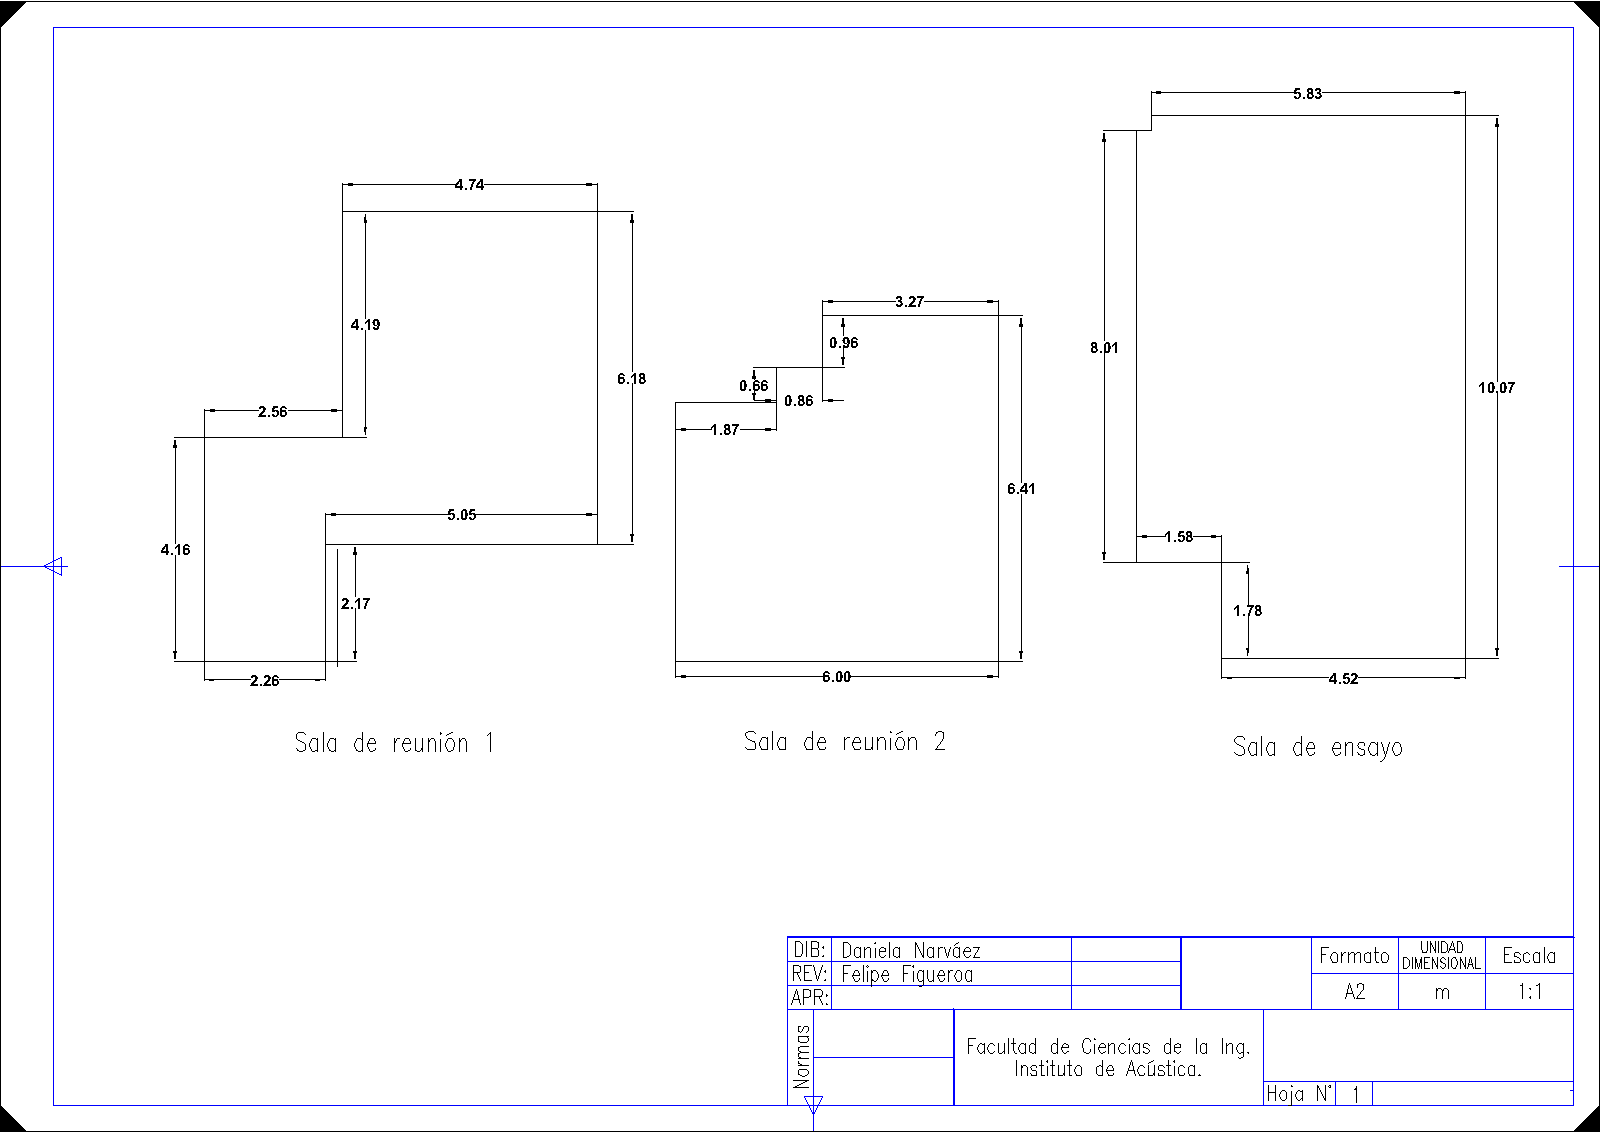
\includegraphics[scale=0.3]{Imagenes/Planos/Planos.png}
    \caption{Planos de salas de reuniones y sala de ensayo Campus los canelos}
    \label{fig: planos CAD}
\end{figure}
%insertar imágenes


\subsection{Medición de parámetros acústicos del recinto}
\noindent Para poder caracterizar acústicamente los salones, se necesita medir parámetros como el ruido de fondo y tiempo de reverberación de cada sala. Para esto se utilizará los siguientes instrumentos:

\begin{table}[H]
    \centering
    \caption{Instrumentación utilizada para las mediciones}
    \label{tab:instrumentacion}
    \resizebox{\textwidth}{!}{%
    \begin{tabular}{|l|l|}
    \hline
    \textbf{Instrumentos} & \textbf{Uso}\\ \hline
    Sonómetro Cirrus CR:$171$B & Medir nivel de presión sonora equivalente \\ \hline
    Micrófono Behringer ECM$8000$ & Recibir el nivel de las fuentes\\\hline
    Conectores XLR & Enviar señal de audio\\ \hline
    Interfaz de audio TASCAM US $4$x$4$ & Procesar señales de audio\\ \hline
    Cinta métrica & Medir distancia de fuente y micrófonos \\ \hline
    Termómetro e higrómetro digital & Medir temperatura y humedad en el lugar de medición\\ \hline
    Protectores auditivos & Proteger oídos de la exposición de sonidos fuertes  \\ \hline
    Notebook con software ARTA & Procesar y analizar señales   \\ \hline
    Globos & Fuente impulsiva \\ \hline
    
    \end{tabular}
    }
\end{table}

\subsubsection{Ruido de fondo}
\noindent Para medir el ruido de fondo se utilizó el sonómetro Cirrus basándose en el 
procedimiento descrito en el D.S. $38/11$, que indica lo siguiente: 
"Se deberá medir el NPSeq en forma continua, hasta que se estabilice la lectura, 
registrando el valor de NPSeq cada 5 minutos. Se entenderá por estabilizada la lectura, 
cuando la diferencia aritmética entre dos registros consecutivos sea menor o igual a $2$ dB(A). 
El nivel a considerar será el último de los niveles registrados. En ningún caso la medición 
deberá extenderse por más de 30 minutos."\cite{ds:ds38}
\begin{figure}[H]
    \centering
    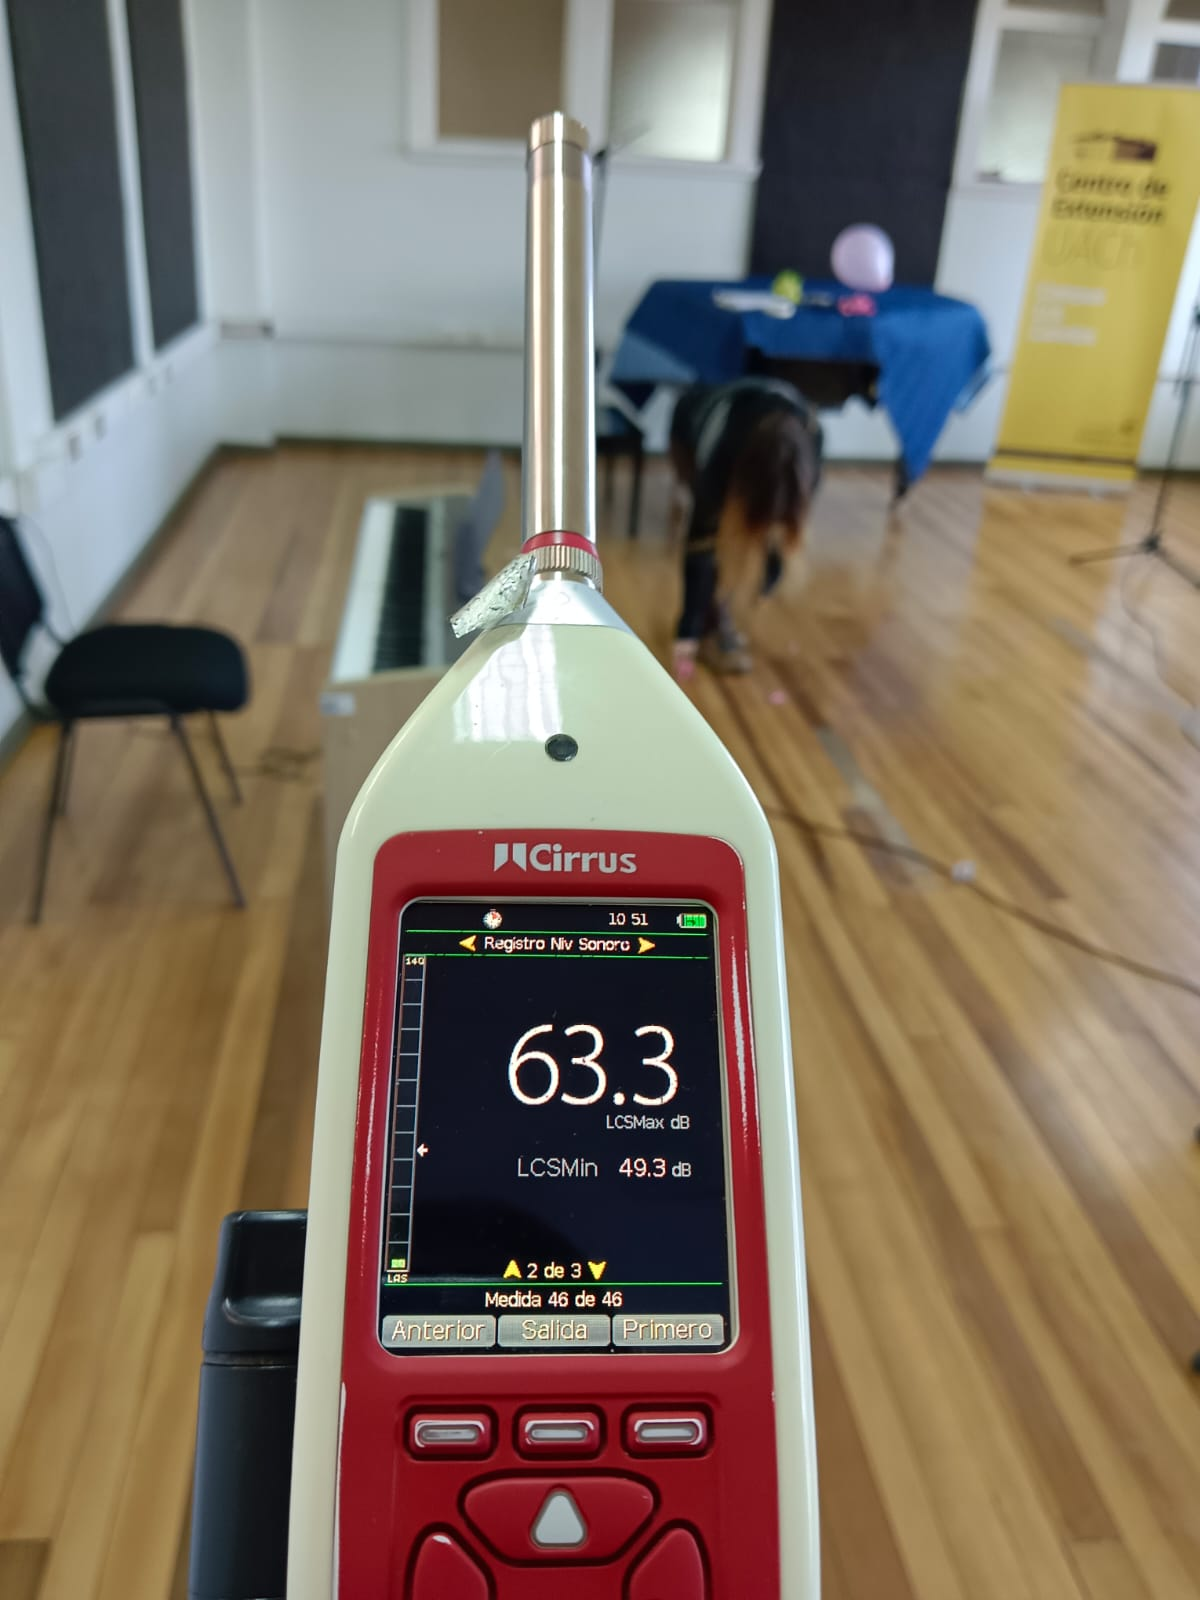
\includegraphics[scale=0.15]{Imagenes/mediciones/medicionRDF.jpeg}
    \caption{Medición de ruido de fondo}
    \label{fig: medicionRDF}
\end{figure}
\subsubsection{Tiempo de reverberación}
\noindent Para la medición de tiempo de reverberación se siguió el procedimiento que indica la norma ISO $3382$-$2$ \cite{ISO3382-2}, utilizando el método de respuesta impulso en cada una de las salas, utilizando globos como fuente impulsiva.
En cada sala de reuniones se realizan dos posiciones de fuente y tres de micrófono, y para la sala de ensayo se utilizan dos posiciones de fuente y cuatro de micrófono, realizando dos mediciones para cada combinación de fuente-micrófono. En el anexo \ref{subsec: posiciones RT} se encuentran los planos con las posiciones de fuente y micrófono utilizadas en cada salón.

\begin{figure}[H]
    \centering
    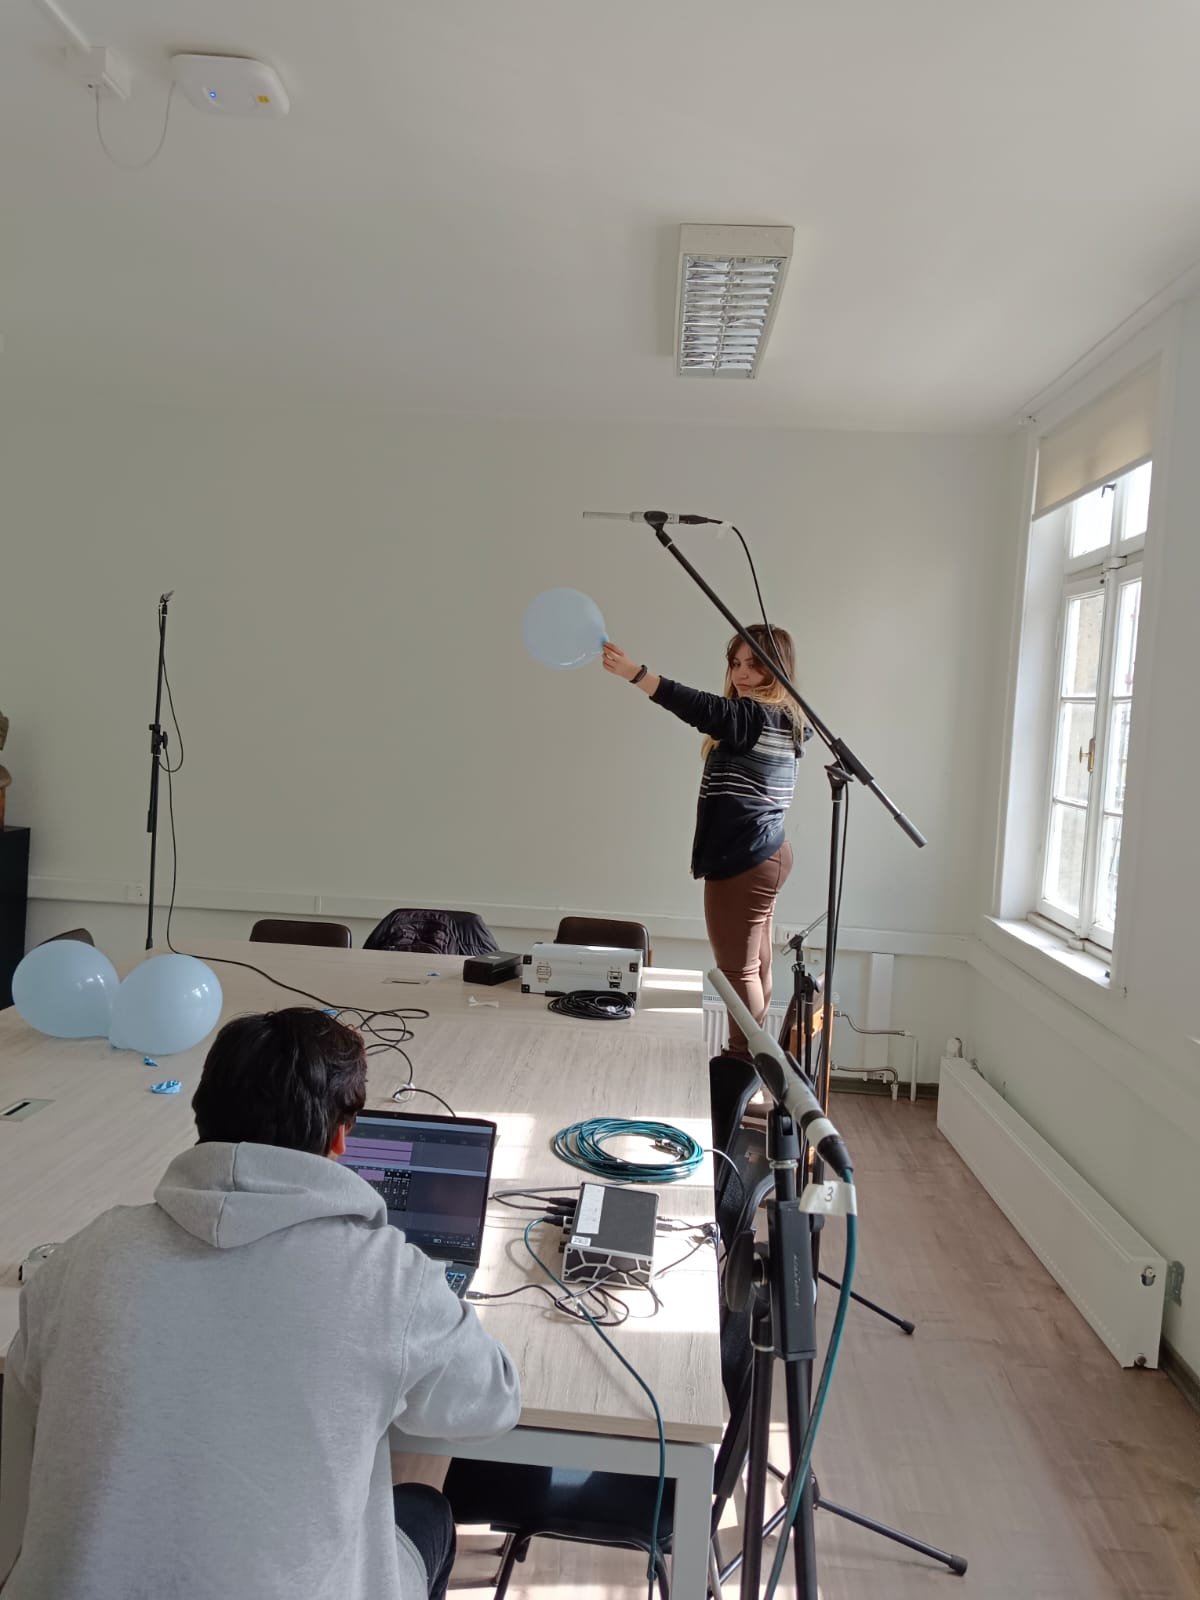
\includegraphics[scale=0.15]{Imagenes/mediciones/medicionRT.jpeg}
    \caption{Medición de ruido de tiempo de reverberación}
    \label{fig: medicionRT}
\end{figure}




\include{Contenido/6.Modelación}
\section{Recomendaciones de parámetros acústicos} \label{secc: Recomendaciones}
Como objetivo de acondicionamiento acústico de cada sala, se consideran recomendaciones de los parámetros antes medidos, los cuales dependen del uso de estas. Por lo que estos se dividen en dos grupos, los que son dirigidos para el uso del habla y otro para la sala dirigida a música clásica.
\subsection{Salas de reuniones}
Para las salas de reuniones se consideran recomendaciones de parámetros determinados para sala de conferencias. En la tabla \ref{tab: parametros objetivos sala de reuniones} se pueden observar los valores objetivo para este tipo de salas y la fuente bibliográfica que determina estos valores.
%inserte tabla
\begin{table}[H]
    \centering
    \begin{tabular}{|c|l|c|l|}
    \hline
    \textbf{Parámetro} & \textbf{Uso }            & \textbf{Valores}    & \textbf{Fuente}  \\ \hline
    Curvas NC          & Para salas de juntas     & $25$ - $30$         & \cite{Recuero} \\ \hline
    $T_{target}$       & Speech/Lecture ($A2$)      & $0.6$               & \cite{DIN18041} \\ \hline
    $C_{50speech}$           & Para la voz              &  $C_{50}>0$         & \cite{marshall1994}  \\ \hline  
    STI & Transmisión del habla & STI $>0.45$ & \cite{ISO9921}\\ \hline
    \end{tabular}
    \caption{Parámetros objetivos para salas de reuniones}
    \label{tab: parametros objetivos sala de reuniones}
\end{table}
\subsection{Sala de ensayo}
Para la sala de ensayo se consideran recomendaciones de parámetros determinados para sala de conciertos de música de cámara, ya que este espacio es utilizado para este tipo de música. En la tabla \ref{tab: parametros objetivos sala de ensayo} se pueden observar los valores objetivo para este tipo de salas y la fuente bibliográfica que determina estos valores.
%inserte tabla
\begin{table}[H]
    \centering
    \begin{tabular}{|c|l|c|c|}
    \hline
    \textbf{Parámetro} & \textbf{Uso}                           & \textbf{Valores} & \textbf{Fuente}  \\ \hline
    Curvas NC          & Salas de conciertos y teatros de ópera & $20$ - $25$      & \cite{Recuero} \\ \hline
    $RT_{mid}$         & Sala de conciertos (música de cámara)  & $1.3$ - $1.7$    & \cite{carrion1990diseno} \\ \hline
    $C_{80}$           & Para música sinfónica                  & $-2<C_{80}<2$    &  \cite{marshall1994}  \\ \hline   
    $D_{50}$           & Salas de concierto                     & $D_{50}<0.5$     &  - \\ \hline
    \end{tabular}
    \caption{Parámetros objetivos para sala de ensayo}
    \label{tab: parametros objetivos sala de ensayo}
\end{table}
\section{Resultados del estado actual de los recintos}
A continuación se muestran los resultados de las mediciones y parámetros más específicos del ruido de fondo y tiempo de reverberación, como curvas NC y NR, claridad ($C_{50speech}$, $C_{80}$) y definición $D_{50}$.
\subsection{Ruido de fondo}
En las figuras \ref{fig: Curvas NC sala 1}, \ref{fig: Curvas NC sala 2} y \ref{fig: Curvas NC sala de ensayo}, se pueden observar los valores obtenidos del ruido de fondo en bandas de octava con su respectiva curva NC más cercana.
    \begin{figure}[H]
        \centering
        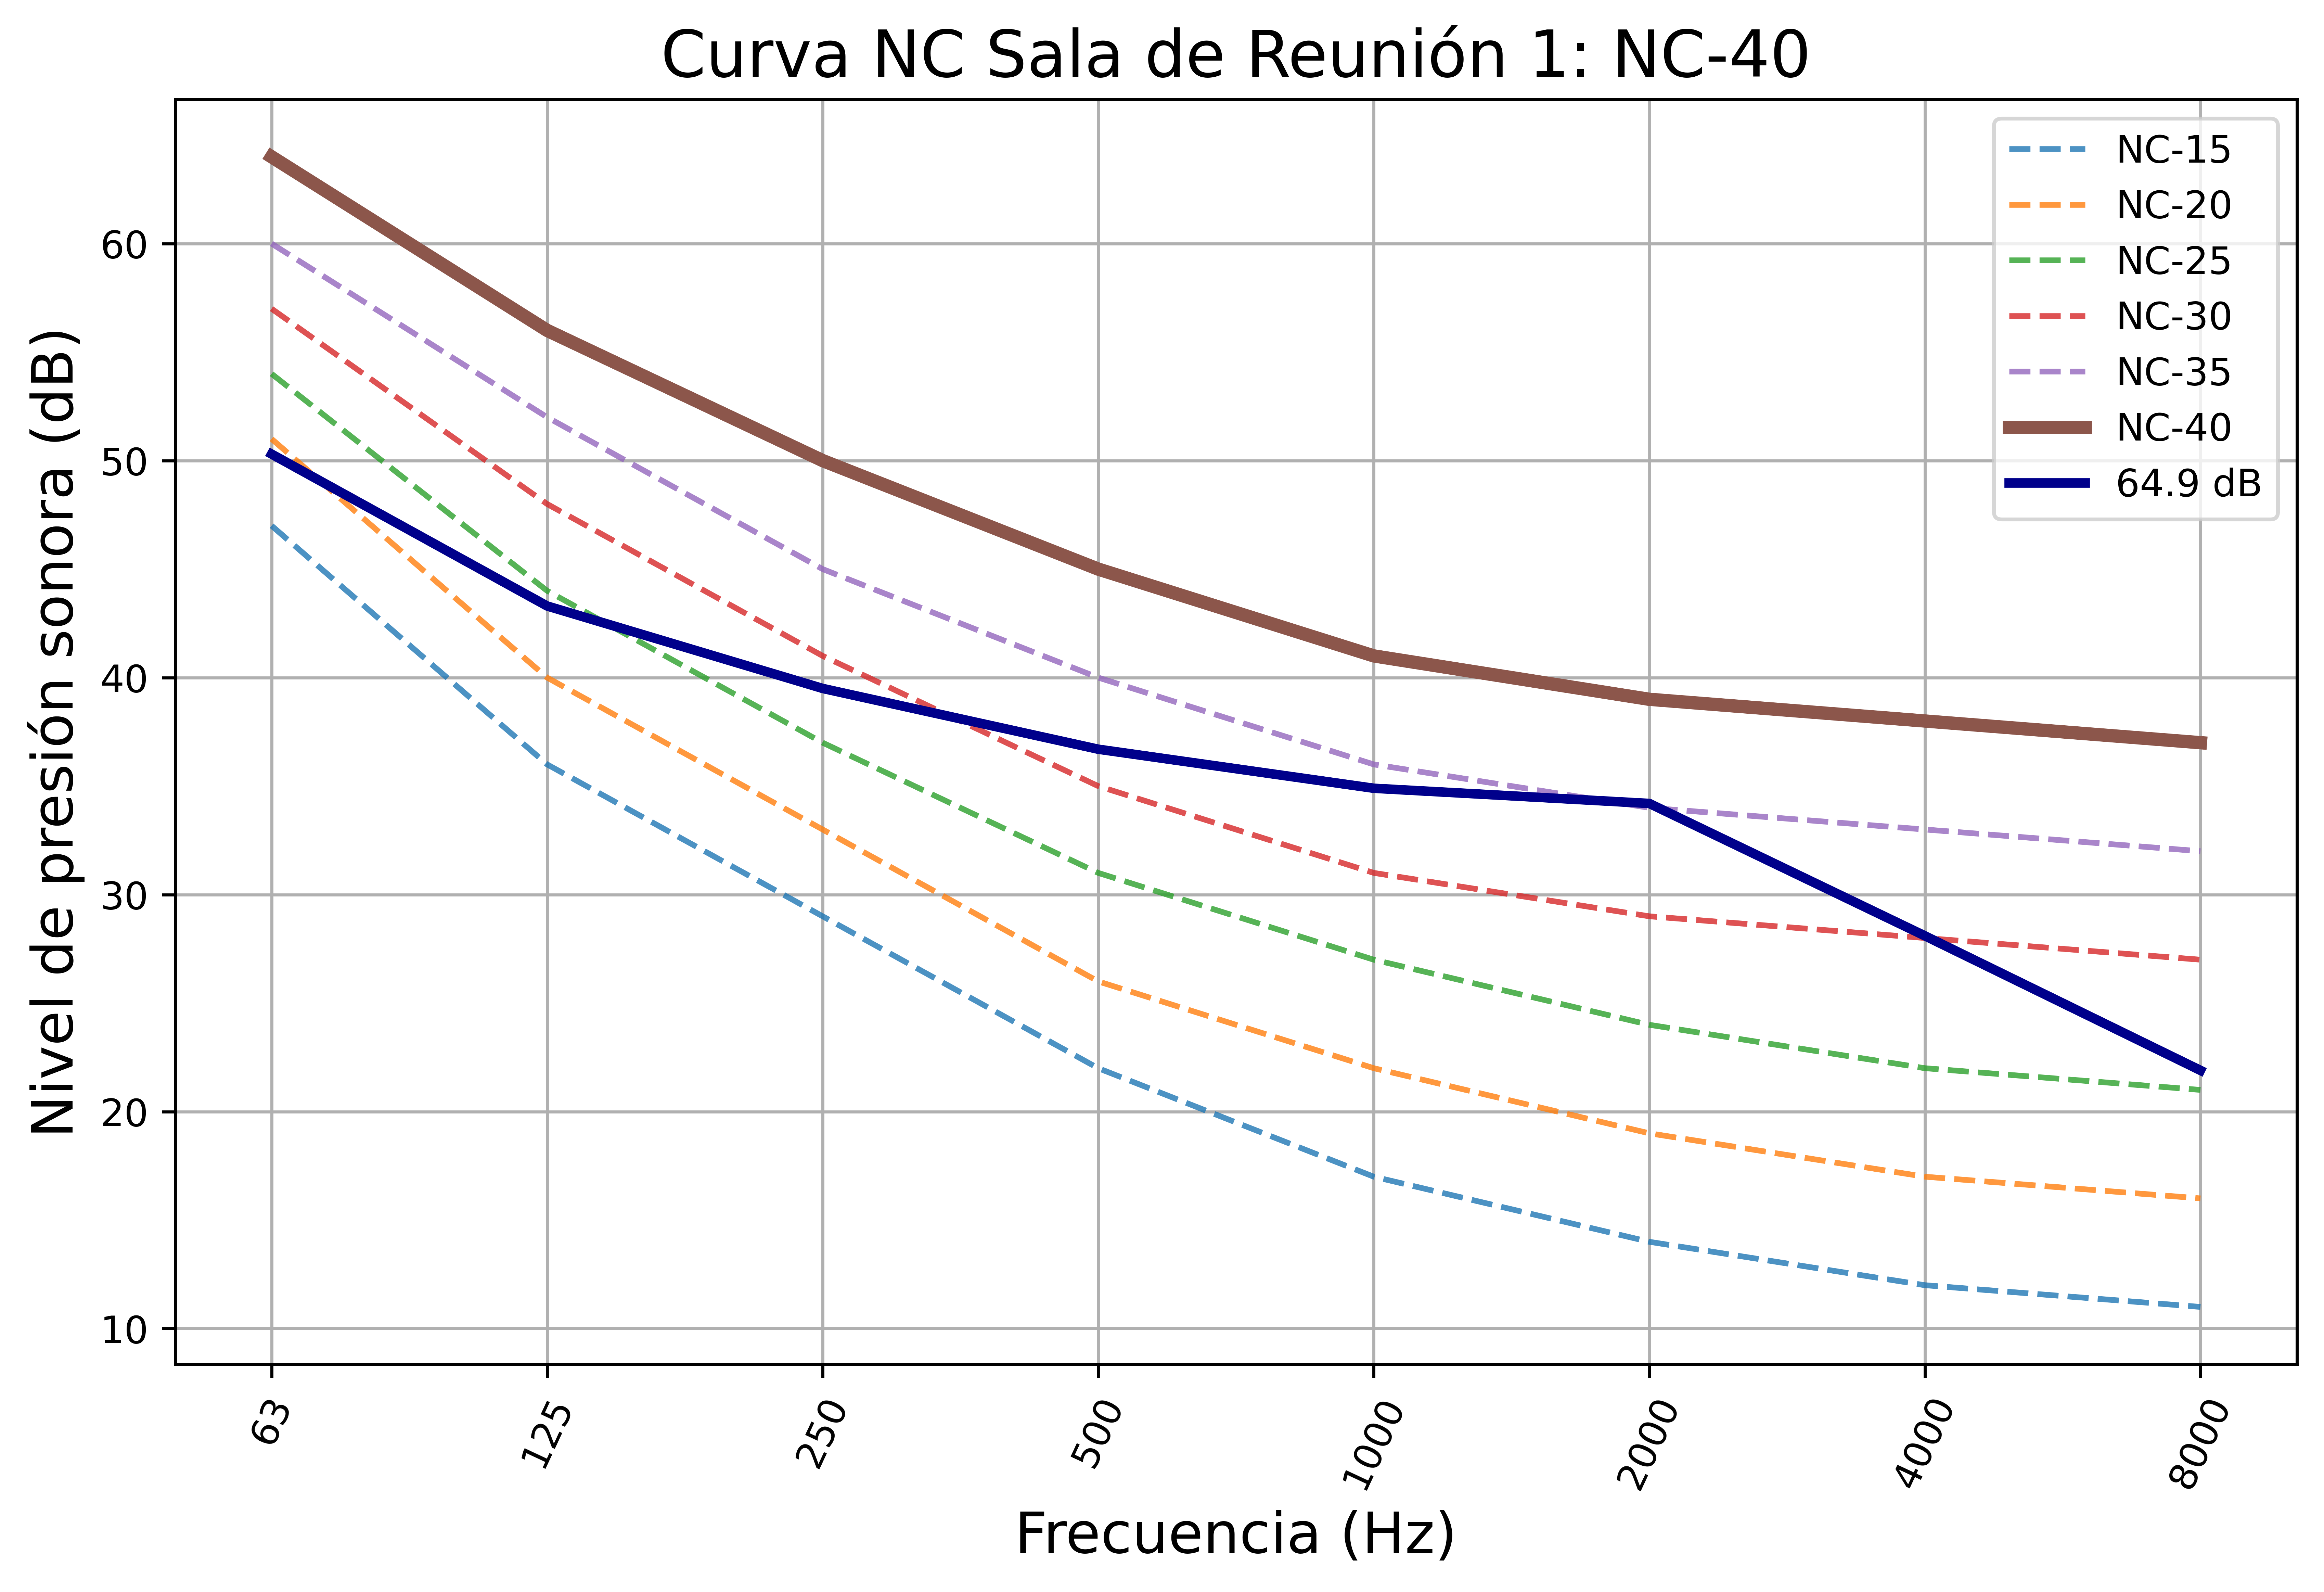
\includegraphics[width=10cm]{Imagenes/Resultados/Curvas NC-NR/NC reunion 1.png}
        \caption{Curvas NC sala de reunión 1}
        \label{fig: Curvas NC sala 1}
    \end{figure}

    \begin{figure}[H]
        \centering
        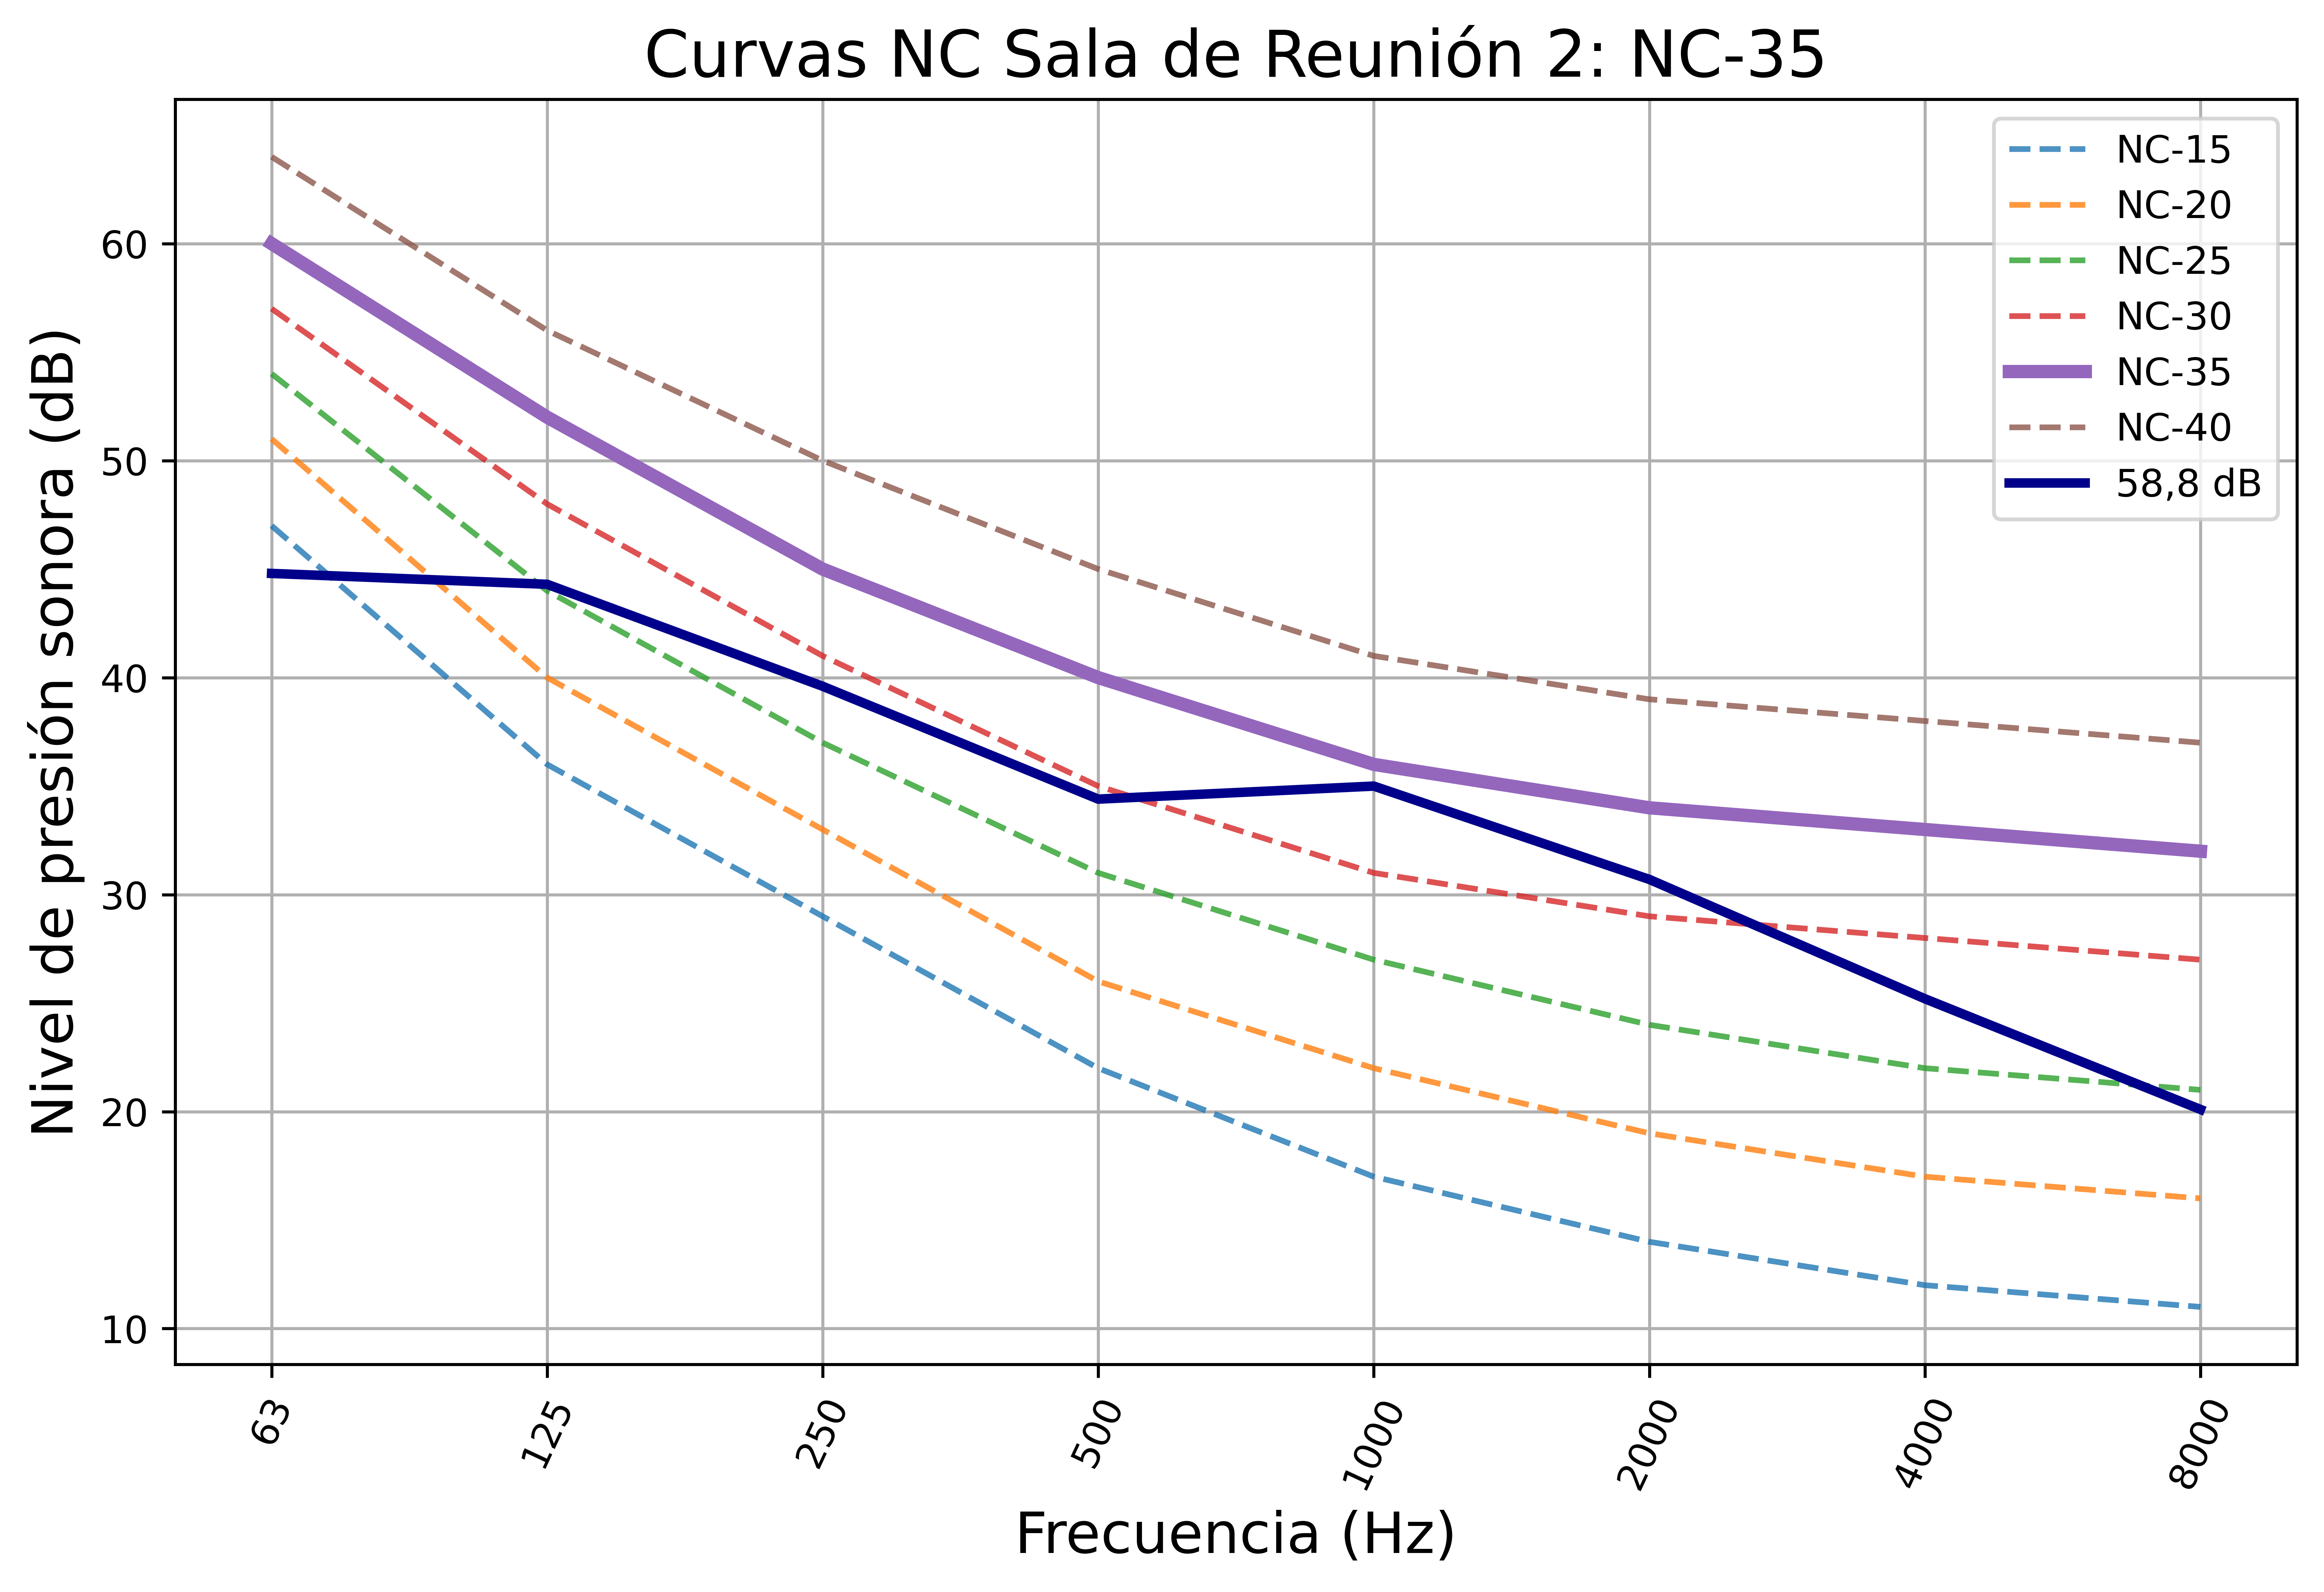
\includegraphics[width=10cm]{Imagenes/Resultados/Curvas NC-NR/NC reunion 2.png}
        \caption{Curvas NC sala de reunión 2}
        \label{fig: Curvas NC sala 2}
    \end{figure}

    \begin{figure}[H]
        \centering
        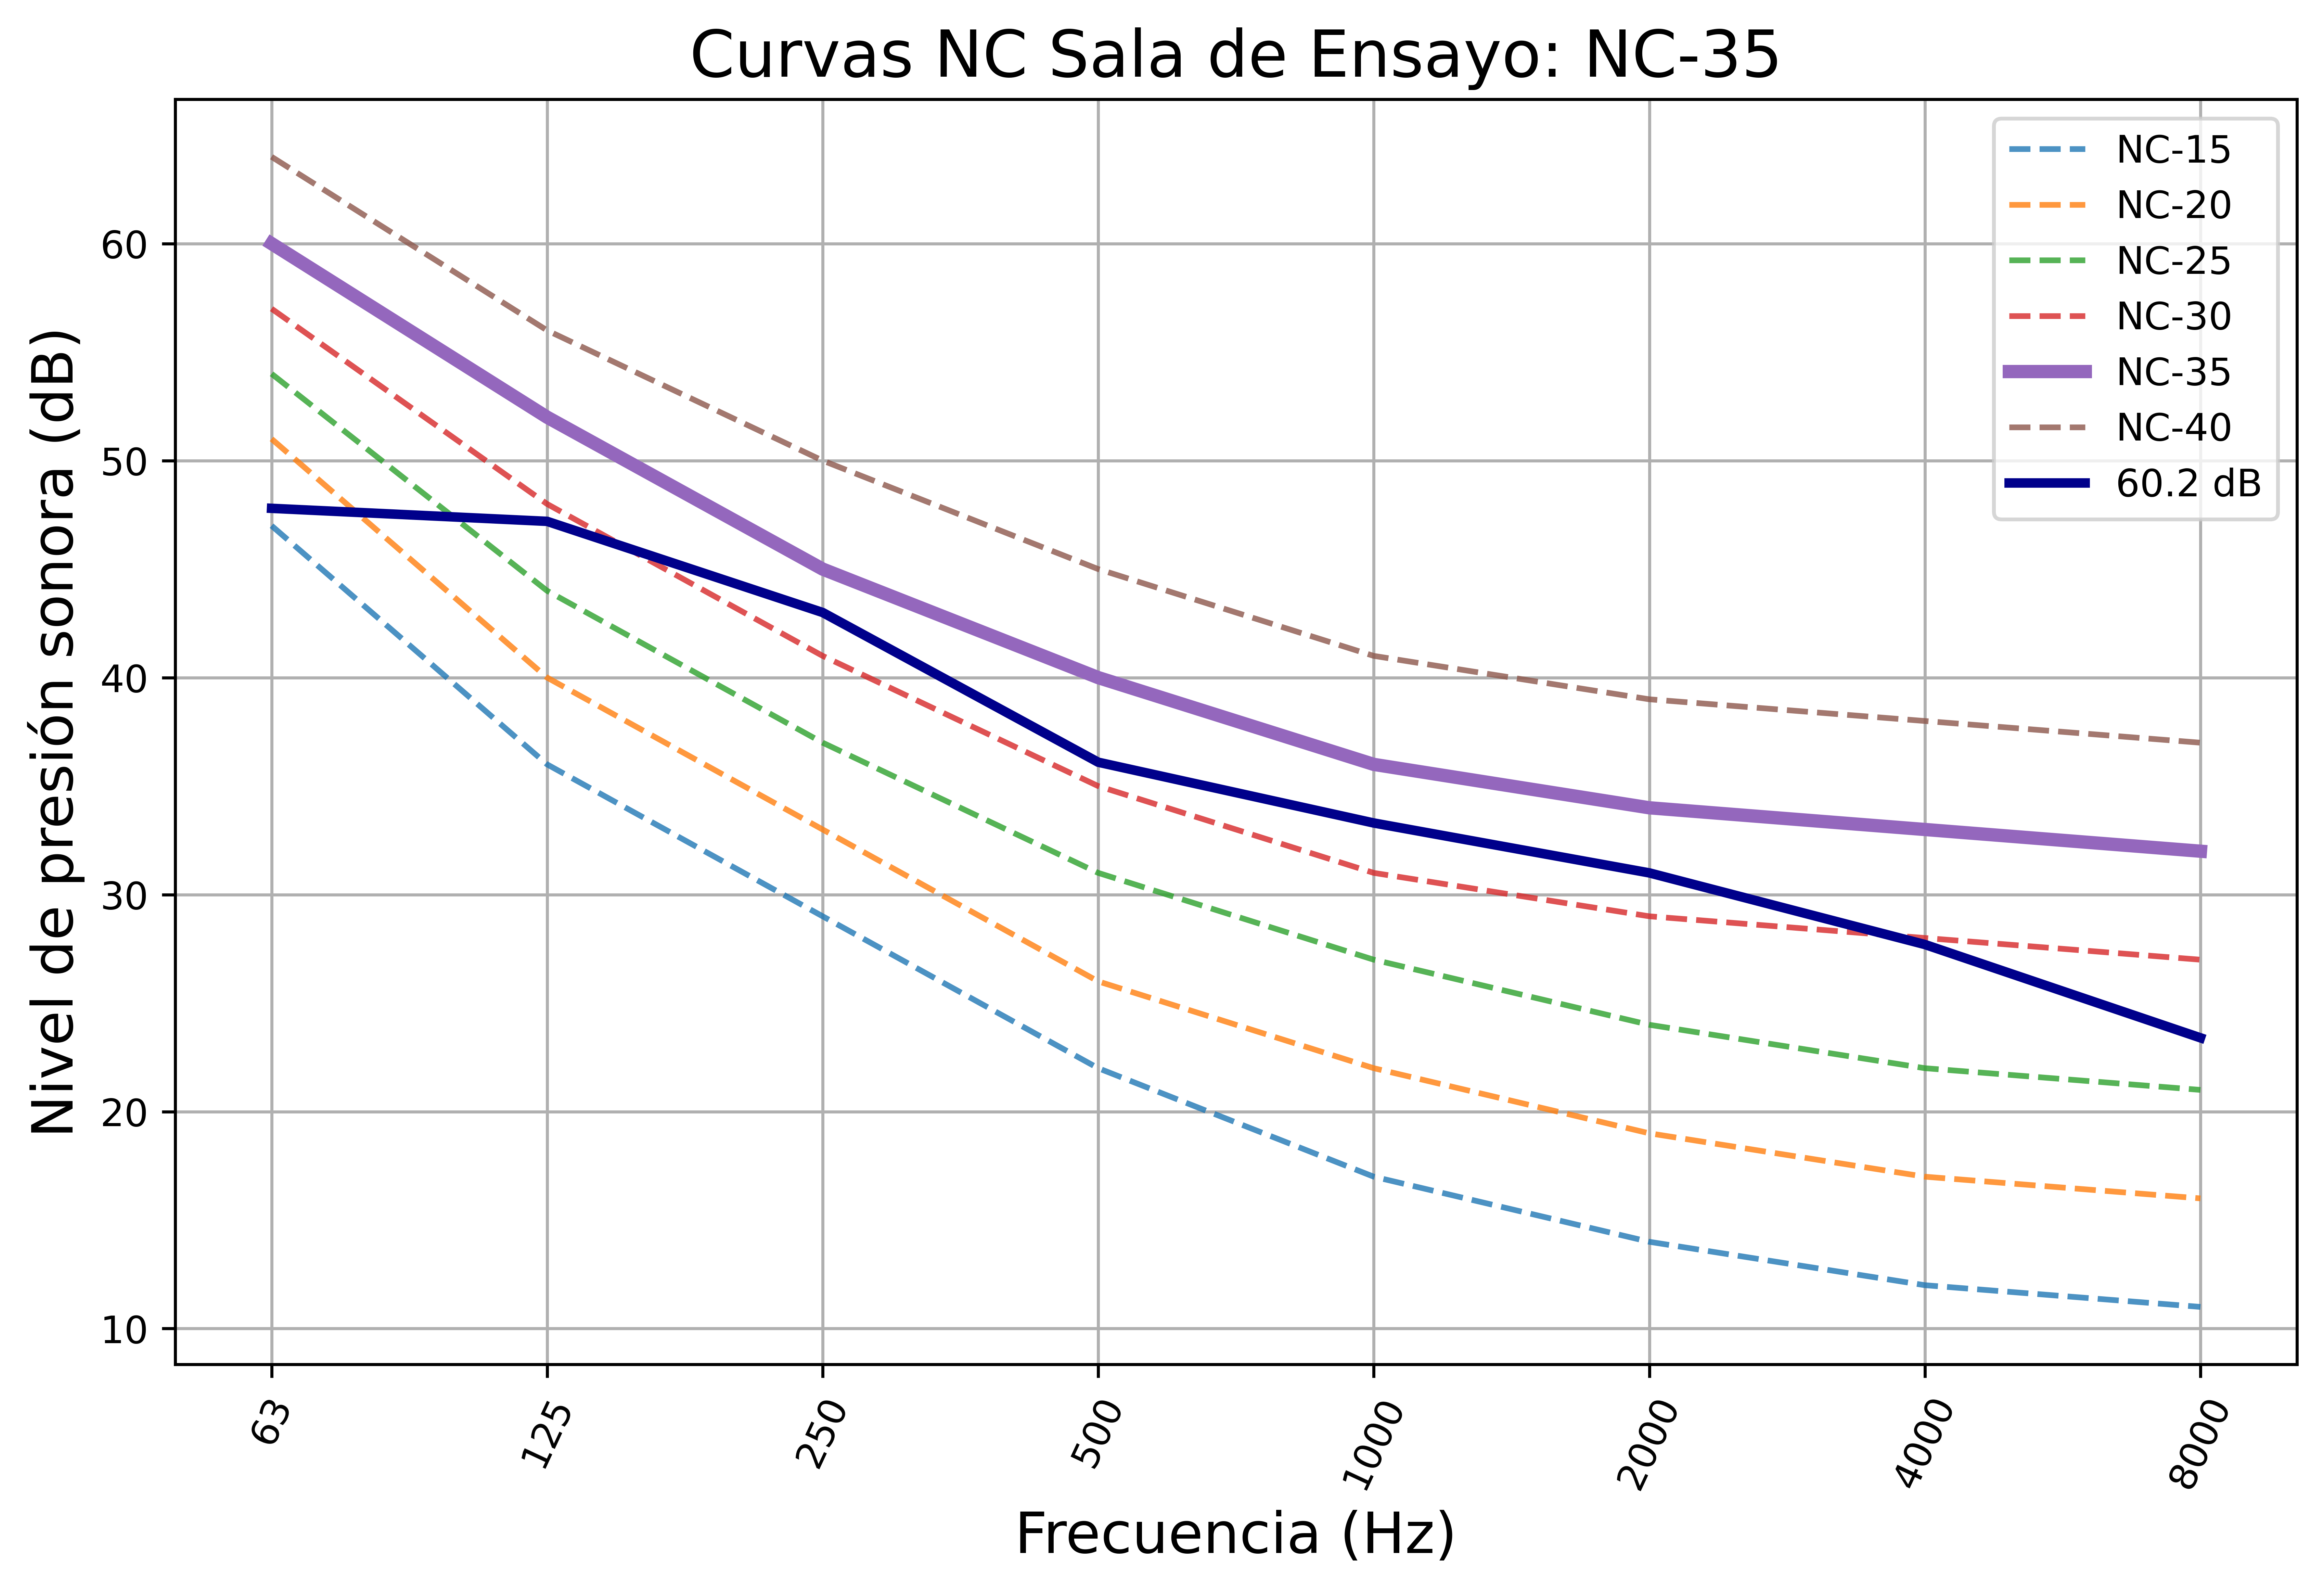
\includegraphics[width=10cm]{Imagenes/Resultados/Curvas NC-NR/NC ensayo.png}
        \caption{Curvas NC sala de ensayo}
        \label{fig: Curvas NC sala de ensayo}
    \end{figure}

Según las recomendaciones mencionadas en la sección \ref{secc: Recomendaciones} se puede determinar que los valores de ruido de fondo como se muestran en la tabla \ref{tab: cumplimiento de Rdf} no cumplen para todas las salas.

\begin{table}[H]
    \centering
    \begin{tabular}{|l|c|c|c|}
    \hline
    \textbf{Salones}  & \textbf{\begin{tabular}[c]{@{}c@{}}Curva NC\\  recomendada\end{tabular}} & \textbf{\begin{tabular}[c]{@{}c@{}}Curva NC\\  medida\end{tabular}} & \textbf{Estado} \\ \hline
    Sala de reunión 1 & $25$ - $30$ & $40$ & \textcolor{red}{No cumple}\\ \hline
    Sala de reunión 2 & $25$ - $30$ & $35$ & \textcolor{red}{No cumple}\\ \hline
    Sala de ensayo    & $20$ - $25$ & $35$ & \textcolor{red}{No cumple} \\ \hline
    \end{tabular}
    \caption{Estado de parámetros de ruido de fondo por sala}
    \label{tab: cumplimiento de Rdf}
    \end{table}

\subsection{Tiempo de reverberación}
\subsubsection{Salas de reunión}
A partir del tiempo de reverberación medido (ver anexo ...), se obtienen los gráficos de tiempo de reverberación descritos en la norma DIN$18041$ para las salas de reunión.
    \begin{figure}[H]
        \centering
        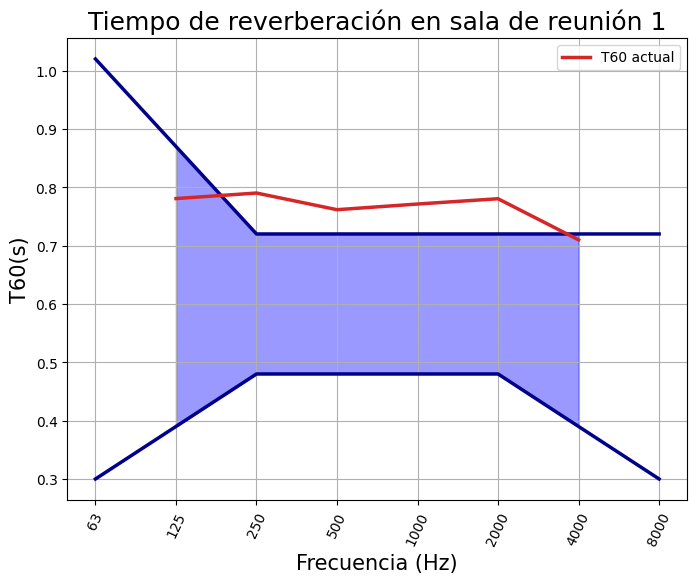
\includegraphics[width=10cm]{Imagenes/DIN/DIN sala reunion 1 actual.png}
        \caption{Tiempo de reverberación Sala de reunión 1}
        \label{fig:Ttarget sala de reunion 1}
    \end{figure}

    \begin{figure}[H]
        \centering
        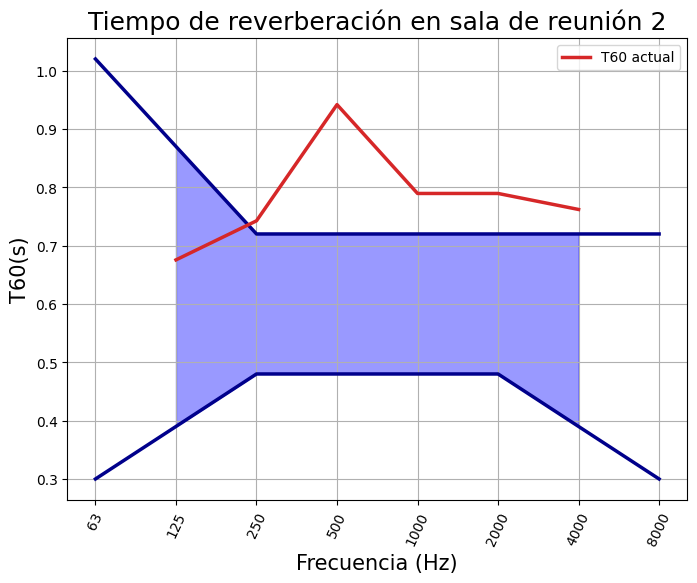
\includegraphics[width=10cm]{Imagenes/DIN/DIN sala reunion 2 actual.png}
        \caption{Tiempo de reverberación Sala de reunión 2}
        \label{fig:Ttarget sala de reunion 2}
    \end{figure}
A continuación se muestra una tabla con los valores obtenidos a partir de las mediciones realizadas. Los gráficos más detallados se encuentran en el anexo.
    %insertar cual anexo
    \begin{table}[H]
        \centering
        \begin{tabular}{|l|c|c|c|}
        \hline
          \textbf{Parámetro}  & \textbf{Recomendación} & \textbf{Sala de reunión $1$} & \textbf{Sala de reunión $2$}\\ \hline
          $T_{target} (s)$    & $0.6$ & \textcolor{red}{No cumple} & \textcolor{red}{No cumple}\\ \hline
          $C_{50speech}$      & $C_{50speech}>0$ & \textcolor{teal}{$1.79$} & \textcolor{teal}{$0.89$} \\ \hline
          STI & STI $> 0.45$  & \textcolor{teal}{$0.66$} & \textcolor{teal}{$0.64$}\\\hline
        \end{tabular}
        \caption{Parámetros acústicos de las salas de reunión}
        \label{tab: cumplimiento parametros RT salas de reuniones}
    \end{table}
\subsubsection{Sala de ensayo}
    Para la sala de ensayo, se determinaron parámetros a partir del tiempo de reverberación, parámetros que se analizaron su cumplimiento con recomendaciones mencionadas en la sección \ref{secc: Recomendaciones}.
    Se obtuvo el siguiente gráfico de definición $D_{50}$:
    \begin{figure}[H]
        \centering
        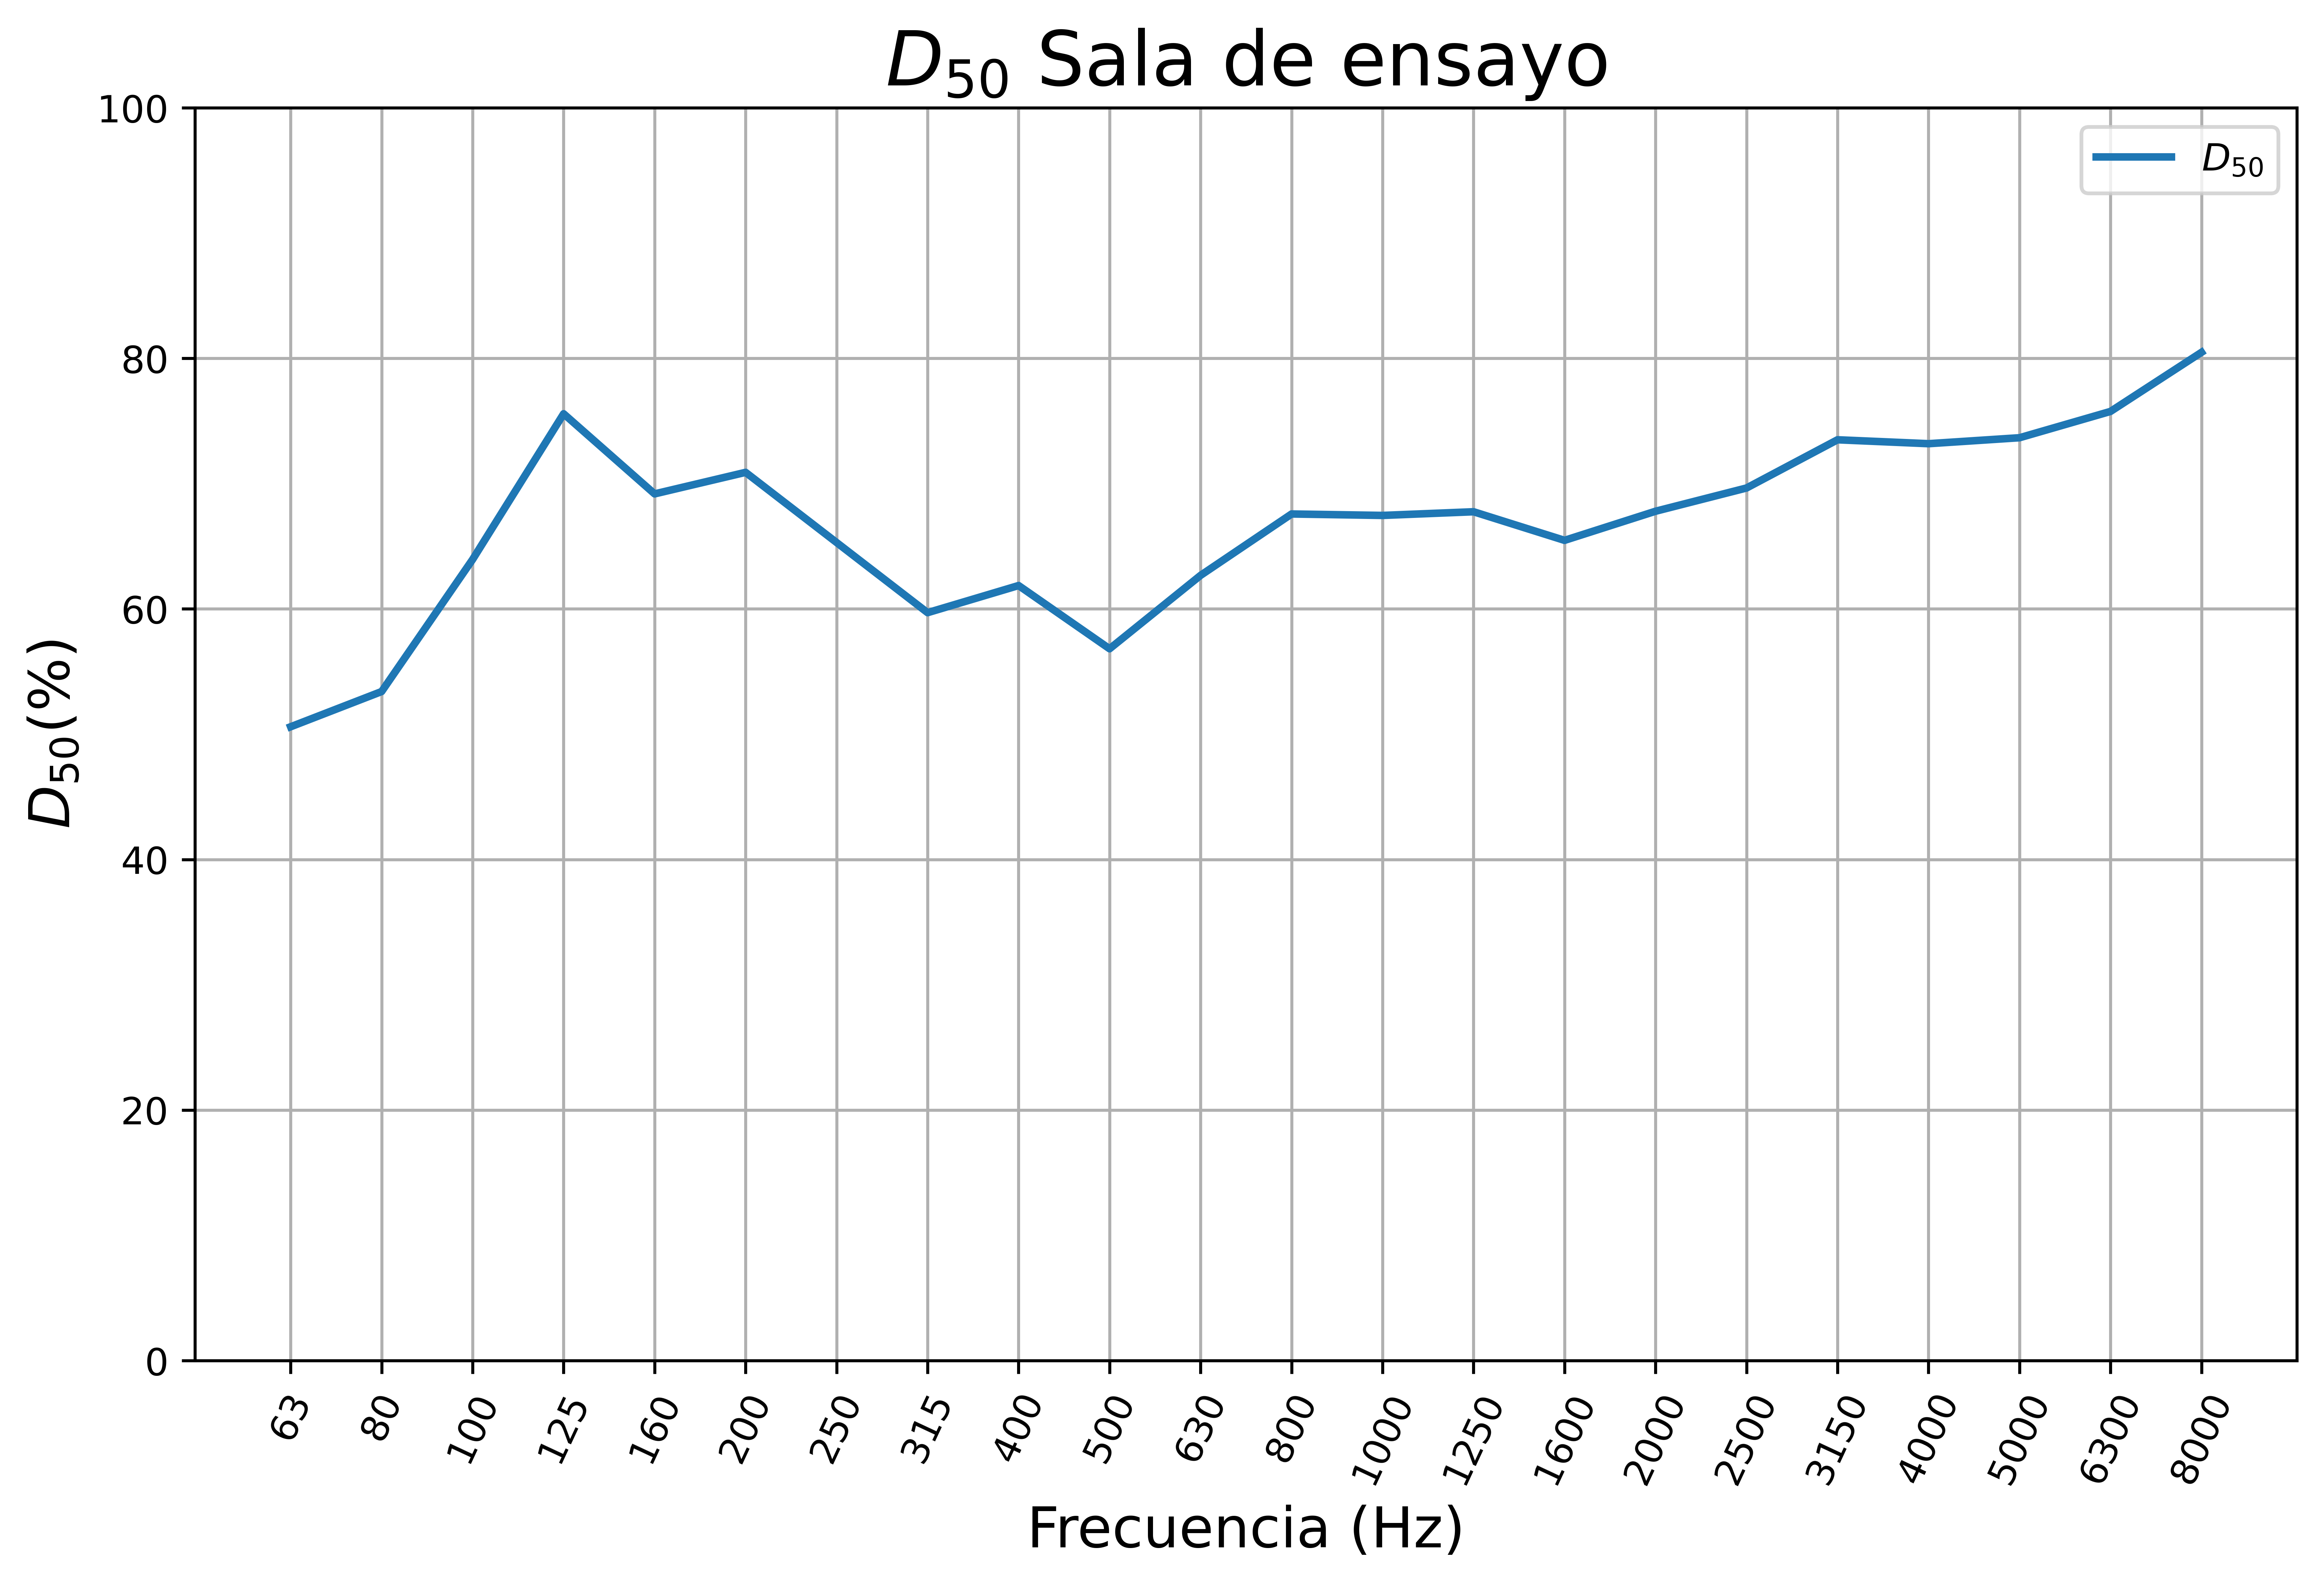
\includegraphics[width=10cm]{Imagenes/Resultados/D50_ensayo.png}
        \caption{$D_{50}$ de sala de ensayo}
    \end{figure}
    En la tabla \ref{tab:parametros acusticos sala ensayo} se puede observar el estado actual de la sala de ensayo determinando su $RT_{mid}$, $C_{80}$ y $D_{50}$.
    \begin{table}[H]
        \centering
        \begin{tabular}{|l|c|c|}
        \hline
        \textbf{Parámetro}& \textbf{Recomendación} & \textbf{Sala de ensayo}\\ \hline
        $RT{mid} (s)$ &  $1.3$ - $1.7$  & \textcolor{red}{$0.74$} \\ \hline
        $C_{80}$      & $-2<C_{80}<2$   & \textcolor{red}{$6.04$} \\\hline
        $D_{50}$      & $D_{50}<$ $0.5$   & \textcolor{red}{No cumple} \\\hline
        \end{tabular}
        \caption{Parámetros acústicos de la sala de ensayo y su estado}
        \label{tab:parametros acusticos sala ensayo}
    \end{table}
\subsection{Análisis modal}
Para observar el estado actual de la sala de ensayo de mejor manera, se hizo un análisis modal. En la figura ... se puede observar la distribución modal de la sala.
%insertar imagen de distribución modal


\section{Propuesta}
\subsection{Salas de reunión}
En las salas de reunión se pudo analizar que el tiempo de reverberación no es el mejor para su utilización según la norma DIN$18041$, por lo que con esta solución se buscará disminuirlo, mejorando la inteligibilidad y la claridad del habla.\\
Para esto se sugiere la aplicación de un panel ranurado en el cielo de cada recinto. Se proponen dos posibles soluciones para cada una de las salas, la cual varia el tamaño del cielo y la cantidad de material absorbente dentro de este.
\subsubsection{Nube}
Para la primera propuesta se sugiere instalar en una sección de cada sala el material ...., donde la superficie en la sala 1 sería de  ... $m^2$ y de .... $m^2$ en la sala 2, como se puede observar en la figura ...

%insertar imagen de nube en sala 1 y 2
\subsection{Sala de ensayo}
Para la sala de ensayo se recomienda extraer el material absorbente que se instaló, cambiando así el tiempo de reverberación favorablemente para el uso que le da al recinto.
%agregar imagen de sala sin paneles.
\section{Resultados de recintos acondicionados}
\subsection{Salas de reunión}
Para el caso de las salas de reunión se obtuvieron los siguientes resultados de ambas propuesta de acondicionamiento. (ver tabla ...)
%insertar tabla con resultados de propuestas y comparándolos con el estado actual
\subsection{Sala de ensayo}
Para el caso de la sala de ensayo se obtuvieron los siguientes resultados. (ver tabla ...)
%insertar tabla con resultados de propuesta y comparándolo con el estado actual
\begin{table}[H]
    \begin{tabular}{|l|l|ll|}
    \hline
     &  & \multicolumn{2}{l|}{\textbf{Sala de ensayo}} \\ \cline{3-4} 
    \multirow{-2}{*}{\textbf{Parámetro}} & \multirow{-2}{*}{\textbf{Recomendación}} & \multicolumn{1}{l|}{\textbf{Estado actual}} & \textbf{Propuesta} \\ \hline
    $RT_{mid}$ & 0.3 - 0.7 & \multicolumn{1}{l|}{\textcolor{red}{0.74}} & \textcolor{teal}{1.4} \\ \hline
    $C_{80}$ & $-2<C_{80}<2$ & \multicolumn{1}{l|}{\textcolor{red}{6.04}} & \textcolor{teal}{3} \\ \hline
    $D_{50}$ & $D_{50}$ \textless 0.5 & \multicolumn{1}{l|}{\textcolor{red}{No cumple}} & \textcolor{red}{No cumple} \\ \hline
    \end{tabular}
    \caption{Parámetros acústicos de la sala de ensayo del estado actual y acondicionado}
    \label{tab: resultados sala de ensayo}
\end{table}
\section{Presupuesto del proyecto}

El costo total de los elementos que componen la propuesta de acondicionamiento acústico presentada se presenta en la Tabla \ref{tab: cotizacion}.
\begin{table}[H]
    \centering
    \caption{Presupuesto de la propuesta de acondicionamiento acústico}
    \label{tab: cotizacion}
    \resizebox{\textwidth}{!}{%
    \begin{tabular}{cccccccc|}
    \cline{2-8}
    \multicolumn{1}{c|}{}                                                             & \multicolumn{7}{c|}{\cellcolor[HTML]{C9DAF8}\textbf{Solución 1: Nube}}                                                                                                                                                                                                                                                                                                                                                                                                 \\ \hline
    \rowcolor[HTML]{EFEFEF} 
    \multicolumn{1}{|c|}{\cellcolor[HTML]{FFF2CC}}                                    & \multicolumn{1}{c|}{\cellcolor[HTML]{EFEFEF}\textbf{Material}} & \multicolumn{1}{c|}{\cellcolor[HTML]{EFEFEF}\textbf{Superficie (u)}} & \multicolumn{1}{c|}{\cellcolor[HTML]{EFEFEF}\textbf{Costo (u)}} & \multicolumn{1}{c|}{\cellcolor[HTML]{EFEFEF}\textbf{Superficie (m2)}} & \multicolumn{1}{c|}{\cellcolor[HTML]{EFEFEF}\textbf{Unidades}} & \multicolumn{1}{c|}{\cellcolor[HTML]{EFEFEF}\textbf{Residuo (m2)}} & \textbf{Costo Total}                           \\ \cline{2-8} 
    \multicolumn{1}{|c|}{\cellcolor[HTML]{FFF2CC}}                                    & \multicolumn{1}{c|}{Volcanita Rigitone $12$/$25$Q}                 & \multicolumn{1}{c|}{$2.4$}                                             & \multicolumn{1}{c|}{CLP $\$63,490$}                              & \multicolumn{1}{c|}{$9$}                                                & \multicolumn{1}{c|}{$4$}                                         & \multicolumn{1}{c|}{$0.60$}                                          & CLP $\$253,960$                                  \\ \cline{2-8} 
    \multicolumn{1}{|c|}{\multirow{-3}{*}{\cellcolor[HTML]{FFF2CC}Sala de reunión $1$}} & \multicolumn{1}{c|}{Aislanglass $60$MM R$100$/$141$}                 & \multicolumn{1}{c|}{$14.4$}                                            & \multicolumn{1}{c|}{CLP $\$44,190$}                               & \multicolumn{1}{c|}{$9$}                                                & \multicolumn{1}{c|}{$1$}                                         & \multicolumn{1}{c|}{$5.40$}                                          & CLP $\$44,190$                                   \\ \hline
                                                                                      & \multicolumn{2}{l}{}                                                                                                                  & \multicolumn{1}{l}{}                                            & \multicolumn{1}{l}{}                                                  & \multicolumn{1}{l}{}                                           & \multicolumn{1}{l|}{}                                              & \textbf{CLP $\$298,150$}                         \\ \hline
    \rowcolor[HTML]{EFEFEF} 
    \multicolumn{1}{|c|}{\cellcolor[HTML]{F4CCCC}}                                    & \multicolumn{1}{c|}{\cellcolor[HTML]{EFEFEF}\textbf{Material}} & \multicolumn{1}{c|}{\cellcolor[HTML]{EFEFEF}\textbf{Superficie (u)}} & \multicolumn{1}{c|}{\cellcolor[HTML]{EFEFEF}\textbf{Costo (u)}} & \multicolumn{1}{c|}{\cellcolor[HTML]{EFEFEF}\textbf{Superficie (m2)}} & \multicolumn{1}{c|}{\cellcolor[HTML]{EFEFEF}\textbf{Unidades}} & \multicolumn{1}{c|}{\cellcolor[HTML]{EFEFEF}\textbf{Residuo (m2)}} & \textbf{Costo Total}                           \\ \cline{2-8} 
    \multicolumn{1}{|c|}{\cellcolor[HTML]{F4CCCC}}                                    & \multicolumn{1}{c|}{Volcanita Rigitone $12$/$25$Q}                 & \multicolumn{1}{c|}{$2.4$}                                             & \multicolumn{1}{c|}{CLP $\$63,490$}                               & \multicolumn{1}{c|}{$12.5$}                                             & \multicolumn{1}{c|}{$5$}                                         & \multicolumn{1}{c|}{$1.90$}                                          & CLP $\$380,940$                                 \\ \cline{2-8} 
    \multicolumn{1}{|c|}{\multirow{-3}{*}{\cellcolor[HTML]{F4CCCC}Sala de reunión $2$}} & \multicolumn{1}{c|}{Aislanglass 60MM R$100$/$141$}                 & \multicolumn{1}{c|}{$14.4$}                                            & \multicolumn{1}{c|}{CLP $\$44,190$}                               & \multicolumn{1}{c|}{$12.5$}                                             & \multicolumn{1}{c|}{$1$}                                         & \multicolumn{1}{c|}{$1.90$}                                          & CLP $\$44,190$                                 \\ \hline
                                                                                      & \multicolumn{2}{l}{}                                                                                                                  & \multicolumn{1}{l}{}                                            & \multicolumn{1}{l}{}                                                  & \multicolumn{1}{l}{}                                           & \multicolumn{1}{l|}{}                                              & \textbf{CLP $\$425,130$}                         \\ \cline{7-8} 
                                                                                      & \multicolumn{1}{l}{}                                           & \multicolumn{1}{l}{}                                                 & \multicolumn{1}{l}{}                                            & \multicolumn{1}{l}{}                                                  & \multicolumn{1}{l|}{}                                          & \multicolumn{1}{c|}{\cellcolor[HTML]{B6D7A8}\textbf{Costo total}}  & \cellcolor[HTML]{B6D7A8}\textbf{CLP $\$723,280$} \\ \cline{7-8} 
    \end{tabular}%
    }
\end{table}
\section{Medición de coeficiente de absorción de un material}
Como actividad extra del proyecto, se realizo el análisis del coeficiente de absorción sonora de una muestra de madera ranurada con lana mineral y lana de vidrio. (ver figura ...)
%insertar imágenes de los materiales

La madera contaba con ranuras de diámetro de $5$mm y una distancia de $10$ mm entre ellas como lo indica la figura ...
%insertar imagen del material medido


Para realizar las mediciones se utilizó un tubo de impedancia con una muestra de cada materiales, combinando primero la madera con lana mineral sin plenum y un plenum de $2$ cm, y lo mismo con la lana de vidrio.\\
A raíz de las mediciones en el tubo se obtuvo el factor de reflexión, del cual se calculó el coeficiente de absorción de cada combinación a través de la formula ... indicada en el anexo ... Los coeficientes obtenidos se pueden observar en el siguiente gráfico de la figura ... y la tabla ...
%añadir grafico de coeficientes y la tabla
\section{Conclusiones}
Se logró cumplir con las actividades propuestas en el cronograma, logrando medir y analizar el estado actual de las
salas, crear una propuesta de mejora en cada uno de los recintos y realizar un presupuesto de estas soluciones.\\
A raíz de los resultados de las mediciones, se logró identificar si estos son adecuados acústicamente para el uso 
de cada uno de estos recintos. Por un lado, el ruido presente en los salones es el problema que predomina, 
incumpliendo con las curvas NC recomendadas para su uso.\\
En el caso del tiempo de reverberación en las salas de reuniones según la norma DIN$18041$ estos no cumplen con 
valores acordes a su uso. Lo cual con la propuesta dada en este proyecto se logró cumplir con este criterio, además
de mejorar la claridad y la inteligibilidad de la palabra en ambas salas.\\
En el caso del tiempo de reverberación de la sala de ensayo, los valores eran demasiado bajos con la implementación
que se realizó por parte de la administración, los valores obtenidos no eran aptos para que el sonido resonara y 
cree intimidad musical, que es lo que se busca en estos recintos. Con la solución de retirar este material, 
aumentaría el tiempo de reverberación, mejorando la claridad y la definición del sonido de los instrumentos.\\

\bibliography{referencias}
\section{Anexo}
\subsection{Presupuesto} 
\noindent A continuación, se muestra el presupuesto a partir de las horas invertidas descritas en la planificación, dando un total de \$ $3.842.227$ pesos. 
\begin{table}[H]
\centering
\caption{Presupuesto del proyecto}
\label{tab: presupuesto}
\resizebox{\columnwidth}{!}{%
\begin{tabular}{clc|c|c|c|}
\hline
\multicolumn{1}{|l|}{} & \multicolumn{1}{l|}{\textbf{Actividades}} & \textbf{Horas} & \textbf{UF/hr} & \textbf{UF*} & \textbf{CLP} \\ \hline
\multicolumn{1}{|c|}{\multirow{8}{*}{\textbf{Costo ingeniería}}} & \multicolumn{1}{l|}{Planificación} & $7$ & $0.6$ & $4.2$ & $151.687$ \\
\multicolumn{1}{|c|}{} & \multicolumn{1}{l|}{Mediciones} & $9$ & $1$ & $9$ & $325.044 $\\
\multicolumn{1}{|c|}{} & \multicolumn{1}{l|}{Modelación} & 1$8 $& $0.8$ & $14.4$ & $520.070$ \\
\multicolumn{1}{|c|}{} & \multicolumn{1}{l|}{Análisis de datos} & $6$ & $1$ & $6$ & $216.696$ \\
\multicolumn{1}{|c|}{} & \multicolumn{1}{l|}{Diseño de propuesta} & $24$ & $1$ & $24$ & $866.784$ \\
\multicolumn{1}{|c|}{} & \multicolumn{1}{l|}{Análisis de propuesta} & $12$ & $0.8$ & $9.6$ & $346.713$ \\
\multicolumn{1}{|c|}{} & \multicolumn{1}{l|}{Cotización de propuesta} & $8$ & $0.6$ & $4.8$ & $173.356$ \\
\multicolumn{1}{|c|}{} & \multicolumn{1}{l|}{Redacción de informe} & $26$ & $0.6$ & $15.6$ & $563.409$ \\ \hline
\multicolumn{1}{|c|}{\multirow{2}{*}{\textbf{Costo operacional}}} & \multicolumn{1}{l|}{Arriendo de equipos} &  &  & $1.7$ & $60.000$ \\
\multicolumn{1}{|c|}{} & \multicolumn{1}{l|}{Traslados} &  &  & $0.1$ & $5.000$ \\ \hline
\multicolumn{1}{l|}{} & \multicolumn{1}{l|}{\textbf{Total}} & $110$ &  & $89.3$ & $3.228.762$ \\ \cline{2-6} 
\multicolumn{1}{l}{} &  &  & IVA ($19$\%) & $17$ & $613.465$ \\ \cline{4-6} 
\multicolumn{1}{l}{} &  &  & Total (con IVA) & $106.3$ & $3.842.227$ \\ \cline{4-6} 
\end{tabular}%
}
\end{table}

*\textit{Considerando el valor en UF correspondiente a la fecha del $28$ de agosto de $2023$ es de \$ $36.116$ CLP.}


\subsection{Marco teórico}
\subsubsection{Ruido de fondo (RdF)}
El ruido de fondo es el sonido presente en una sala cuando no hay actividad o no está presente la fuente a evaluar. Este ruido puede ser causado por sistemas de climatización, instalaciones eléctricas o hidráulicas, e incluso ruido externo como el tráfico.

\begin{itemize}

    \item \textbf{Curvas NC}: son curvas de referencia que representan los límites de ruido aceptables en un espacio según su uso. Un recinto se considera que cumple una especificación NC determinada (por ejemplo, NC-$15$, NC-$20$, etc.) cuando los niveles de ruido de fondo, medidos en diferentes bandas de frecuencia, están por debajo de la curva NC correspondiente para todas las frecuencias entre $63$ Hz y $8$ kHz (ver figura \ref{fig:curvas NC}).\cite{carrion1990diseno}
    \begin{figure}[H]
        \centering
        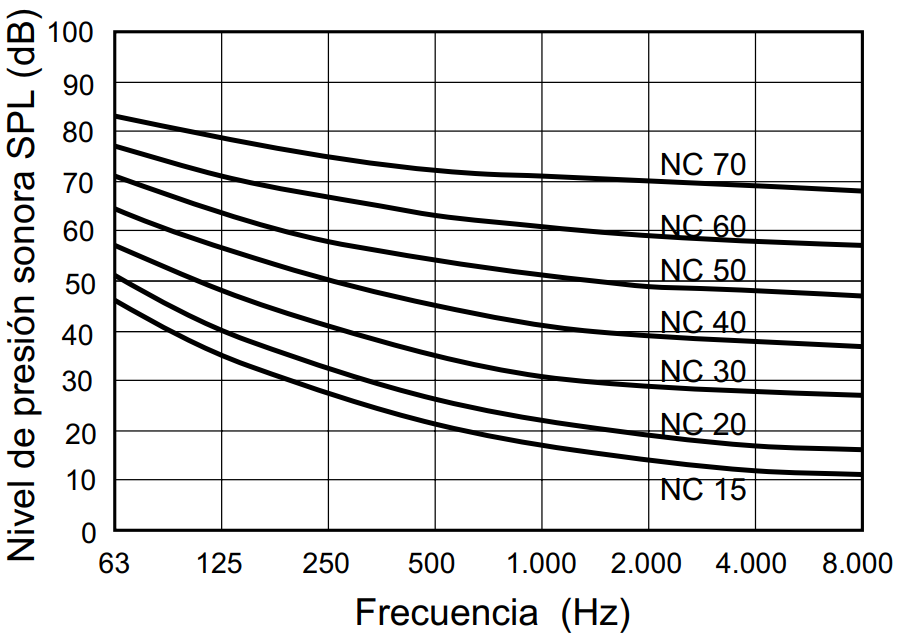
\includegraphics[width=8cm]{Imagenes/MarcoTeorico/CurvaNC.png}
        \caption{Curvas NC (``Noise Criteria'')}
        \label{fig:curvas NC}
    \end{figure}
    En la tabla \ref{tab:recomendaciones Curva NC} se muestran las curvas NC recomendadas para diferentes tipos de recinto, junto con su equivalencia en dBA.
    \begin{table}[H]
        \centering
        \caption{Curvas NC recomendadas y niveles de ruido de fondo equivalentes en dBA }
        \label{tab:recomendaciones Curva NC}
        \begin{tabular}{|l|c|}
        \hline
        \textbf{Tipos de recinto} & \textbf{\begin{tabular}[c]{@{}l@{}}Curva NC\\ recomendada\end{tabular}} \\ \hline
        Fábricas para ingeniería pesada & $55$ - $75$ \\ \hline
        Fábricas para ingeniería ligera & $45$ - $65$ \\ \hline
        Cocinas industriales & $40$ - $50$ \\ \hline
        Recintos deportivos y piscinas & $35$ - $50$ \\ \hline
        Grandes almacenes y tiendas & $35$ - $45$\\ \hline
        Restaurantes, bares, cafeterías y cafeterías privadas & $35$ - $50$  \\ \hline
        Oficinas mecanizadas & $40$ - $50$  \\ \hline
        Oficinas generales & $35$ - $45$  \\ \hline
        Despachos, bibliotecas, salas de justicia y aulas & $30$ - $35$ \\ \hline
        viviendas, dormitorios & $25$ - $35$ \\ \hline
        Salas de hospitales y quirófanos & $25$ - $35$  \\ \hline
        Cines & $30$ - $35$\\ \hline
        Teatros, salas de juntas, iglesias & $25$ - $30$ \\ \hline
        Salas de conciertos y teatros de ópera & $20$ - $25$ \\ \hline
        Estudios de registro y reproducción sonora & $15$ - $20$ \\ \hline
        \end{tabular}
    \end{table}

    \item \textbf{Curvas NR}: Las curvas NR son estándares que muestran los niveles de ruido de fondo aceptables en recintos. Se dividen en números NR (como NR-15, NR-25, NR-35), que indican el nivel máximo de ruido permitido en decibelios (dB) según el propósito del espacio.
En la figura \ref{NR}, se muestran las curvas NR de evaluación de ruido y en la tabla \ref{tabla} , figuran los valores recomendados del índice de NR para diferentes locales.\cite{Recuero}

\begin{figure}[H]
    \centering 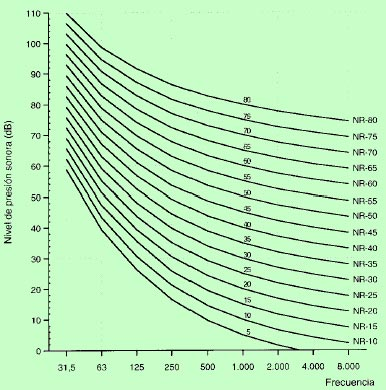
\includegraphics[scale=0.6]{Imagenes/MarcoTeorico/NR.jpg}
    \caption{Curvas NR}
    \label{NR}
\end{figure}

\begin{table}[H]
\centering
\caption{Valores recomendados de índice NR para distintos locales.}
\label{Valores recomendados de NR}
\resizebox{15 cm}{!}{%
\begin{tabular}{|l|c|}
\hline
\multicolumn{1}{|c|}{\textbf{Tipos de recintos}}                                                       & \textbf{Rangos de niveles NR} \\ \hline
Talleres                                                                                               & $60$ - $70$                       \\ \hline
Oficinas mecanizadas                                                                                   & $50$ - $55$                       \\ \hline
Gimnasios, piscinas, salas de deporte, pasillos                                                                  & $40$ - $50$                       \\ \hline
Restaurantes, bares y cafeterías                                                                       & $35$ - $45$                       \\ \hline
Despachos, bibliotecas, salas de justicias                                                             & $30$ - $40$                       \\ \hline
\begin{tabular}[c]{@{}l@{}}Cines, hospitales, iglesias, pequeñas salas y aulas de conferencias \end{tabular} & $25$ - $35$                       \\ \hline
\begin{tabular}[c]{@{}l@{}}Estudio de televisión, grandes salas de conferencias\end{tabular} & $20$ - $30$                       \\ \hline
Sala de conciertos, teatros                                                                            & $20$ - $25$                       \\ \hline
Clínicas, recintos para audiometrías                                                                   & $10$ - $20$                       \\ \hline
\end{tabular}%
}
\label{tabla}
\end{table}
    
\end{itemize}

\subsubsection{Tiempo de reverberación (TR)}
El tiempo de reverberación $T_{60}$ es el tiempo que tarda el sonido en decaer $60$ dB en un espacio cerrado. Este parámetro es importante en el diseño de un sistema de refuerzo sonoro, ya que afecta la claridad, inteligibilidad y calidad del sonido en un recinto.

\begin{itemize}
    \item $T_{30}$: Es una expresión del $T_{60}$ que mide el tiempo que demora el sonido en decaer $30$ dB. El valor $T_{30}$ se entrega ya multiplicado por el factor correcto para medir la que sería la caída por $60$ dB.
    \item Formula de Sabine: Uno de los modelos para calcular el tiempo de reverberación es la fórmula de Sabine. La cual es calculada según lo indicado en la ecuación \ref{eq:T60}. \cite{sabine1922collected}
    \begin{equation} \label{eq:T60} 
     T_{60}=0.161 \cdot \frac{V_{t}}{S_{t} \bar{\alpha}}
    \end{equation}

    donde:
    \begin{itemize}
        \item $V_t$ es el volumen total de la sala
        \item $S_t$ es la superficie total de la sala
        \item $\bar{\alpha}$ es la absorción media de la sala
\end{itemize}
    \item $RT_{mid}$: Es la media aritmética de los valores de tiempo de reverberación correspondientes a las bandas de $500$ Hz y $1$ kHz. En general, el valor más adecuado de $RT_{mid}$ depende del volumen del recinto y de la actividad a la que este destinado este. En la tabla \ref{tab:rtmid recomendado por tipo de sala} se muestran valores recomendados de $RT_{mid}$, para diferentes tipos de salas en el supuesto que estén ocupadas. \cite{carrion1990diseno}
    \begin{table}[H]
        \centering
        \begin{tabular}{|l|c|}
        \hline
             \textbf{Tipo de sala} &  $RT_{mid}$\textbf{, sala ocupada}\\ \hline
             Sala de conferencia& 
             $0.7$ - $1.0$\\
             Cine             & $1.0$ - $1.2$\\
             Sala polivalente & $1.2$ - $1.5$\\
             Teatro de ópera & $1.2$ - $1.5$\\
             Sala de conciertos (música de cámara) & $1.3$ - $1.7$\\
             Sala de conciertos (música sinfónica) & $1.8$ - $2.0$\\
             Iglesia/catedral (órgano y canto coral) & $2.0$ - $3.0$\\
             Locutorio de radio & $0.2$ - $0.4$\\ \hline
        \end{tabular}
        \caption{Valores de $RT_{mid}$ recomendados en función del tipo de sala (recintos ocupados)}
        \label{tab:rtmid recomendado por tipo de sala}
    \end{table}
    En el caso de salas de salas de conferencia/aulas el $RT_{mid}$ recomendado, considerando volúmenes entre los $100$ y $10000$ $m^3$, es entre los valores de:
    \[0.7 \leq RT_{mid} \leq 1 s \]

    \item Claridad: La claridad se refiere a cómo se distribuye la energía del sonido en un espacio. En términos simples, se mide la relación entre el sonido directo y las primeras reflexiones (llamada energía temprana) en comparación con la energía que llega después. En acústica, se utiliza el parámetro $C_{50}$ para evaluar la claridad en entornos destinados a la voz y el $C_{80}$ para la música. Estos valores se obtienen de manera logarítmica y se calculan para un rango de frecuencias entre $125$ y $4000$ Hz.\cite{carrion1990diseno}
    \begin{equation}
      C_{50}= 10 log_{10} \left[\int_0^{50 ms}[g(t)]^2 dt/\int_{50 ms}^{\infty}[g(t)]^2 dt\right]  
    \end{equation}
    \begin{equation}
      C_{80}= 10 log_{10} \left[\int_0^{80 ms}[g(t)]^2 dt/\int_{80 ms}^{\infty}[g(t)]^2 dt\right]  
    \end{equation}
    Marshall, define valores apropiados de $C_{50}$ para el habla y $C_{80}$ para distintos tipos de música, descritos en la figura \ref{fig:Recomendaciones C50 C80} \cite{marshall1994}
    \begin{figure}[H]
        \centering
        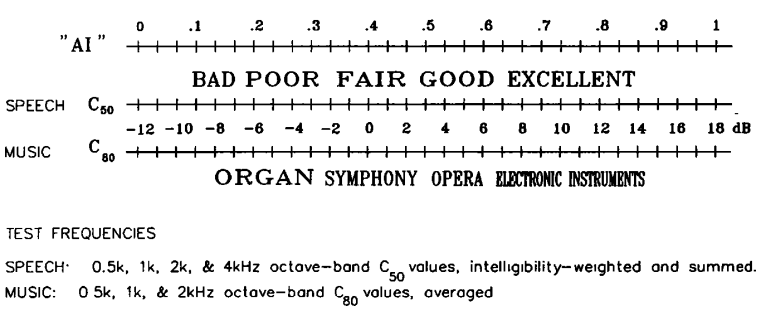
\includegraphics[scale=0.5]{Imagenes/MarcoTeorico/Recomendaciones C50-C80.png}
        \caption{Recomendaciones de claridad para el habla y música}
        \label{fig:Recomendaciones C50 C80}
    \end{figure}
    \item Definición: El parámetro llamado definición se determinó para evaluar la cantidad de energía temprana, el cual se deriva directamente de la respuesta impulso $g(t)$ en la siguiente ecuación:
    \begin{equation}
        D_{50}= \left[\int_0^{50 ms}[g(t)]^2 dt/\int_{0}^{\infty}[g(t)]^2 dt\right] 
    \end{equation}
    Ambas integrales deben incluir el sonido directo, cuya llegada al oyente determina el tiempo $t = 0$. Obviamente, D será del $100\%$ si la respuesta al impulso no contiene componentes con retardos superiores a $50$ ms. \cite{Kuttruff_2017} 

    %insertar figura de Relación entre inteligibilidad de sílabas y definición.
    
    \item STI: Es el índice de transmisión del habla el cual indica el entendimiento de la palabra y sus valores oscilan entre los $0$ y $1$, que evalúa la inteligibilidad en el recinto, siendo los valores cercanos a 0 deficientes y los valores cercanos a $1$ una inteligibilidad excelente. Según la normativa ISO $9921$ \cite{ISO9921} los valores clasificarían como se indica en la tabla \ref{tab: rango STI}. 

\begin{table}[H]
    \centering
    \caption{Rango de STI según ISO $9921$}
    \label{tab: rango STI}
    \begin{tabular}{|c|c|}
    \hline
    \textbf{Rango de inteligibilidad} & \textbf{STI} \\ \hline
    Excelente                &     $>0.75$     \\ \hline
    Bueno                    & $0.60$ - $0.75$ \\ \hline
    Razonable                & $0.45$ - $0.60$ \\ \hline
    Pobre                    & $0.30$ - $0.45$ \\ \hline
    Malo                     & $<0.3$ \\ \hline
    \end{tabular}
\end{table}
\end{itemize}

\subsubsection{Modos normales}
Un modo normal puede ser considerado como una resonancia en el aire de un recinto en una cierta frecuencia modal \cite{Kleiner2014-fd}.
En el espectro de frecuencias bajas, los modos pueden ser identificados por un peak en la curva de respuesta de frecuencia de un recinto, como se puede ver en la Figura \ref{fig: respuesta frecuencia}. 
Esto debido a que la densidad modal es proporcional al cuadrado de la frecuencia, por lo que a mayor frecuencia existe mayor traslape de estos modos.
Este énfasis o supresión de ciertas frecuencias debido al recinto produce una coloración del sonido recibido por un receptor \cite{Kuttruff_2017}.

\begin{figure}[H]
    \centering
    \includegraphics[width=10cm]{Imagenes/MarcoTeorico/respuesta_frecuencias.jpg}
    \caption{Respuesta en frecuencias bajas de un recinto.}
    \label{fig: respuesta frecuencia}
\end{figure}

\subsubsection{Medición de coeficiente de absorción en tubo de impedancia}
Un método utilizado para determinar el coeficiente de absorción acústica de un material es a través del empleo de un tubo de impedancia, también conocido como tubo de Kundt. Este dispositivo consta de un tubo equipado con dos micrófonos dispuestos a lo largo de su longitud, junto con un altavoz ubicado en uno de sus extremos. En el extremo opuesto se sitúa el material cuya capacidad de absorción acústica se pretende medir.
\begin{figure}[H]
    \centering
    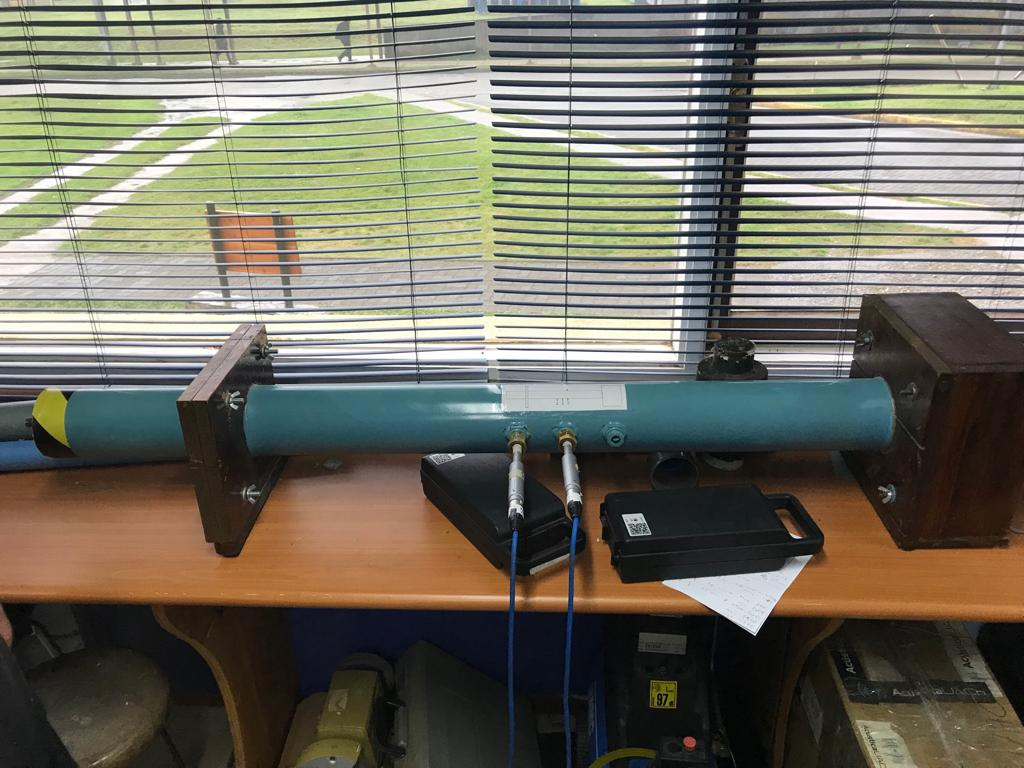
\includegraphics[width=10cm]{Imagenes/Medición abs/TuboImpedancia.jpeg}
    \caption{Tubo de Kundt}
    \label{fig: Tubo de Kundt}
\end{figure}
A partir de la relación de la señal recibida por cada uno de los micrófonos el software ... entrega el coeficiente de reflexión ... el cual se utiliza en la ecuación... para calcular el coeficiente de absorción.
\begin{equation} \label{eq: alpha}
    \alpha = 1 - |r|^2 = 1 - r_{r}^2 - r_{i}^2
\end{equation}
donde,\\
$r$ es el factor de reflexión.\\
$r_{r}$ es el componente real del factor de reflexión.\\
$r_{i}$ es el componente imaginario del factor de reflexión.\cite{ISO10534-2}\\
Posteriormente a la obtención de los datos se realiza el cálculo de los valores de coeficientes de
absorción ponderado, para esto fue necesario transformar los datos obtenidos anteriormente a tercios
de octava y así calcular el coeficiente de absorción sonora práctico ($\alpha_{pi}$), que se define como el valor
del coeficiente de absorción acústica dependiente de la frecuencia, basado en mediciones por bandas
de un tercio de octava, que se obtiene mediante la siguiente fórmula:
\begin{equation}
    \alpha_{pi} = \frac{\alpha_{i1} + \alpha_{i2} + \alpha_{i3}}{3}
\end{equation}
Ahora con los coeficiente de absorción práctico, se obtienen los valores de coeficiente de absorción
ponderado $\alpha_{\omega}$, utilizando la curva de referencia de la figura \ref{fig: curva de referencia} Se irá ajustando la curva de referencia
por intervalos de $0.05$ hacia el valor calculado hasta que la suma de las desviaciones desfavorables
sea menor o igual que $0.10$, esto ocurre cuando el valor medido es menor que el valor de la curva de
referencia. \cite{ISO11654}
\begin{figure}[H]
    \centering
    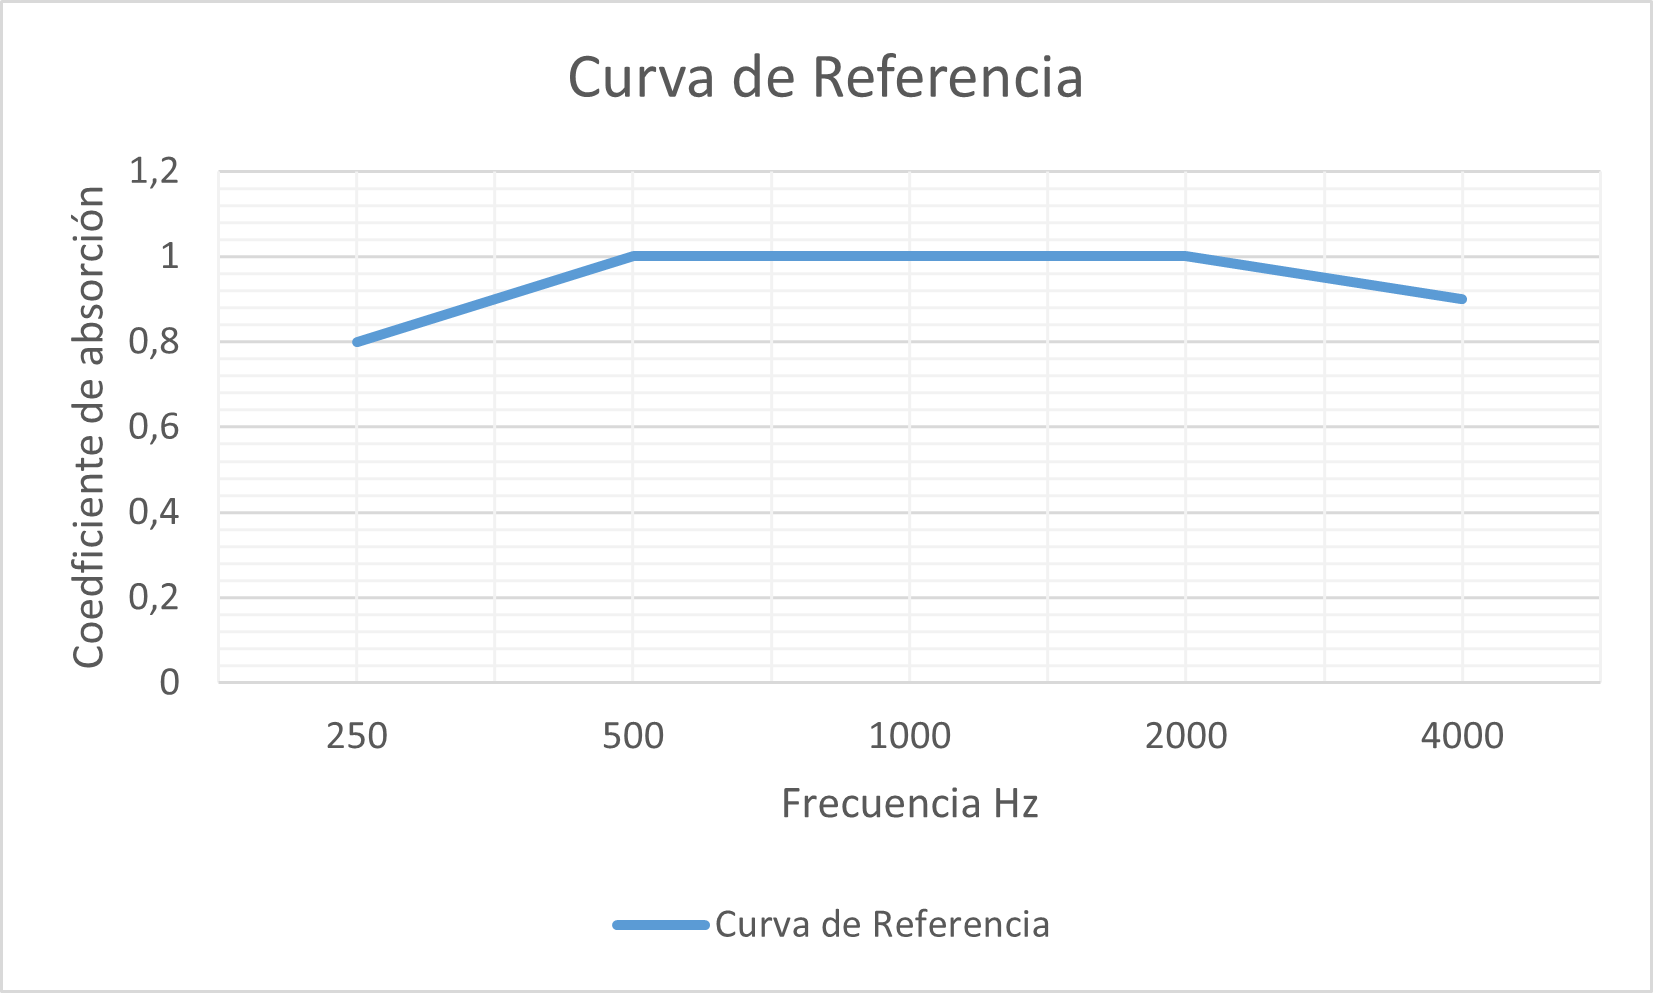
\includegraphics[width=10cm]{Imagenes/Medición abs/curva de referencia.png}
    \caption{Curva de referencia de la medida de coeficiente de absorción}
    \label{fig: curva de referencia}
\end{figure}

\subsection{Posiciones de micrófono y fuente en mediciones de tiempo de reverberación} \label{subsec: posiciones RT}
A continuación se pueden observar la distribución de las posiciones de fuente y micrófono para las mediciones de tiempo de reverberación.
\begin{figure}[H]
    \centering
    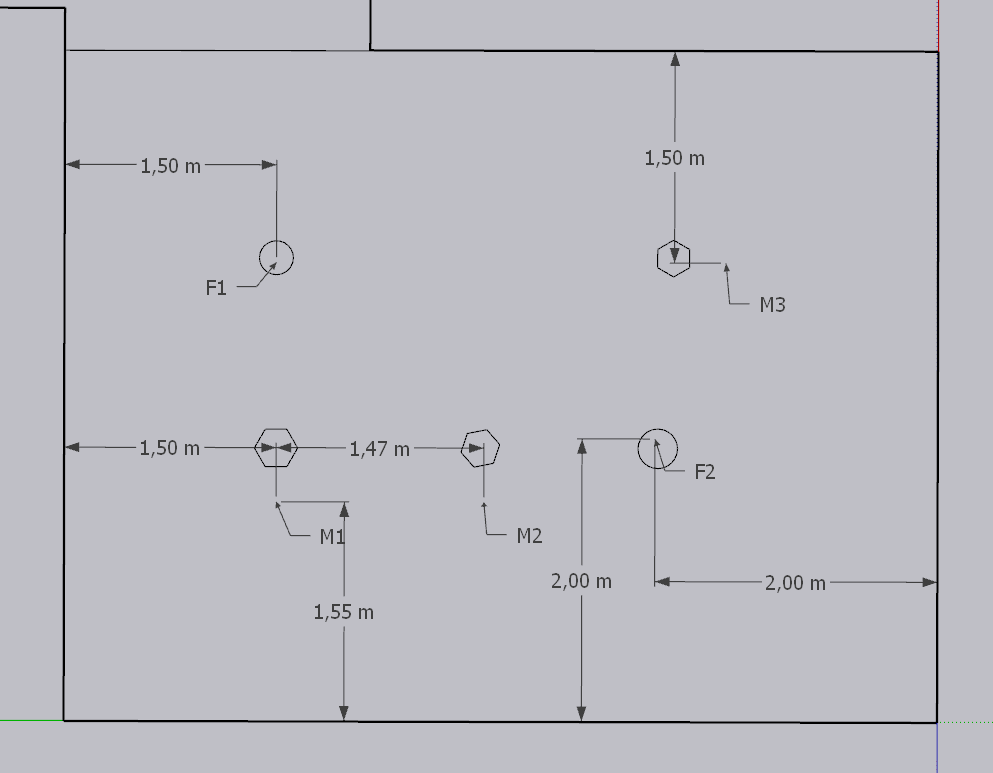
\includegraphics[scale=0.4]{Imagenes/PosicionesRT/Posiciones Sala 1.png}
    \caption{Posiciones de fuente y micrófono para sala de reunión 1}
    \label{fig: posiciones sala1}
\end{figure}

\begin{figure}[H]
    \centering
    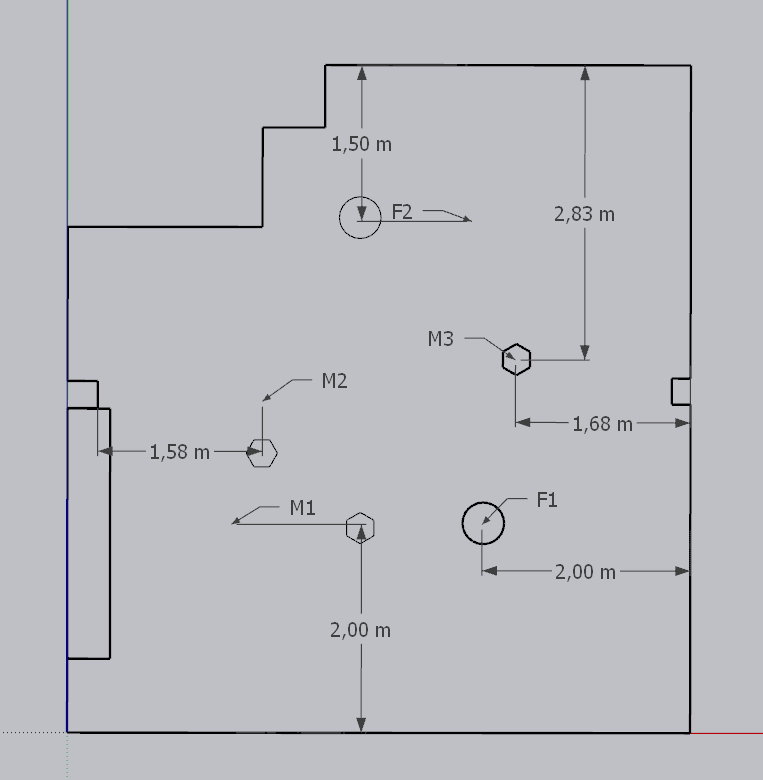
\includegraphics[scale=0.4]{Imagenes/PosicionesRT/Posiciones Sala 2.png}
    \caption{Posiciones de fuente y micrófono para sala de reunión 2}
    \label{fig: posiciones sala2}
\end{figure}

\begin{figure}[H]
    \centering
    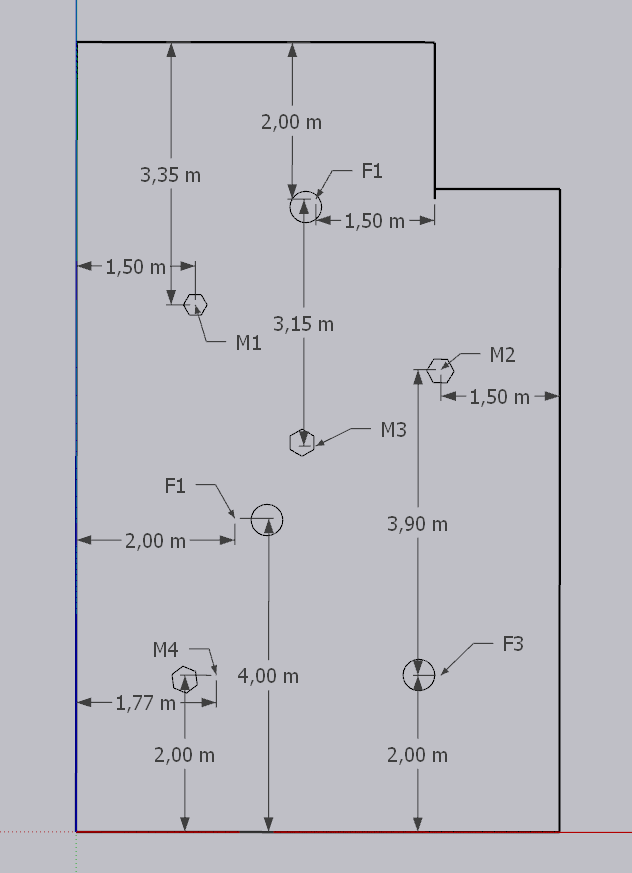
\includegraphics[scale=0.4]{Imagenes/PosicionesRT/Posiciones Sala OCV.png}
    \caption{Posiciones de fuente y micrófono para sala de ensayo}
    \label{fig: posiciones sala OCV}
\end{figure}

\subsection{Mediciones de tiempo de reverberación}
A continuación se pueden observar los resultados de cada posición de micrófono y fuente de tiempo de reverberación
\begin{figure}[H]
    \centering
    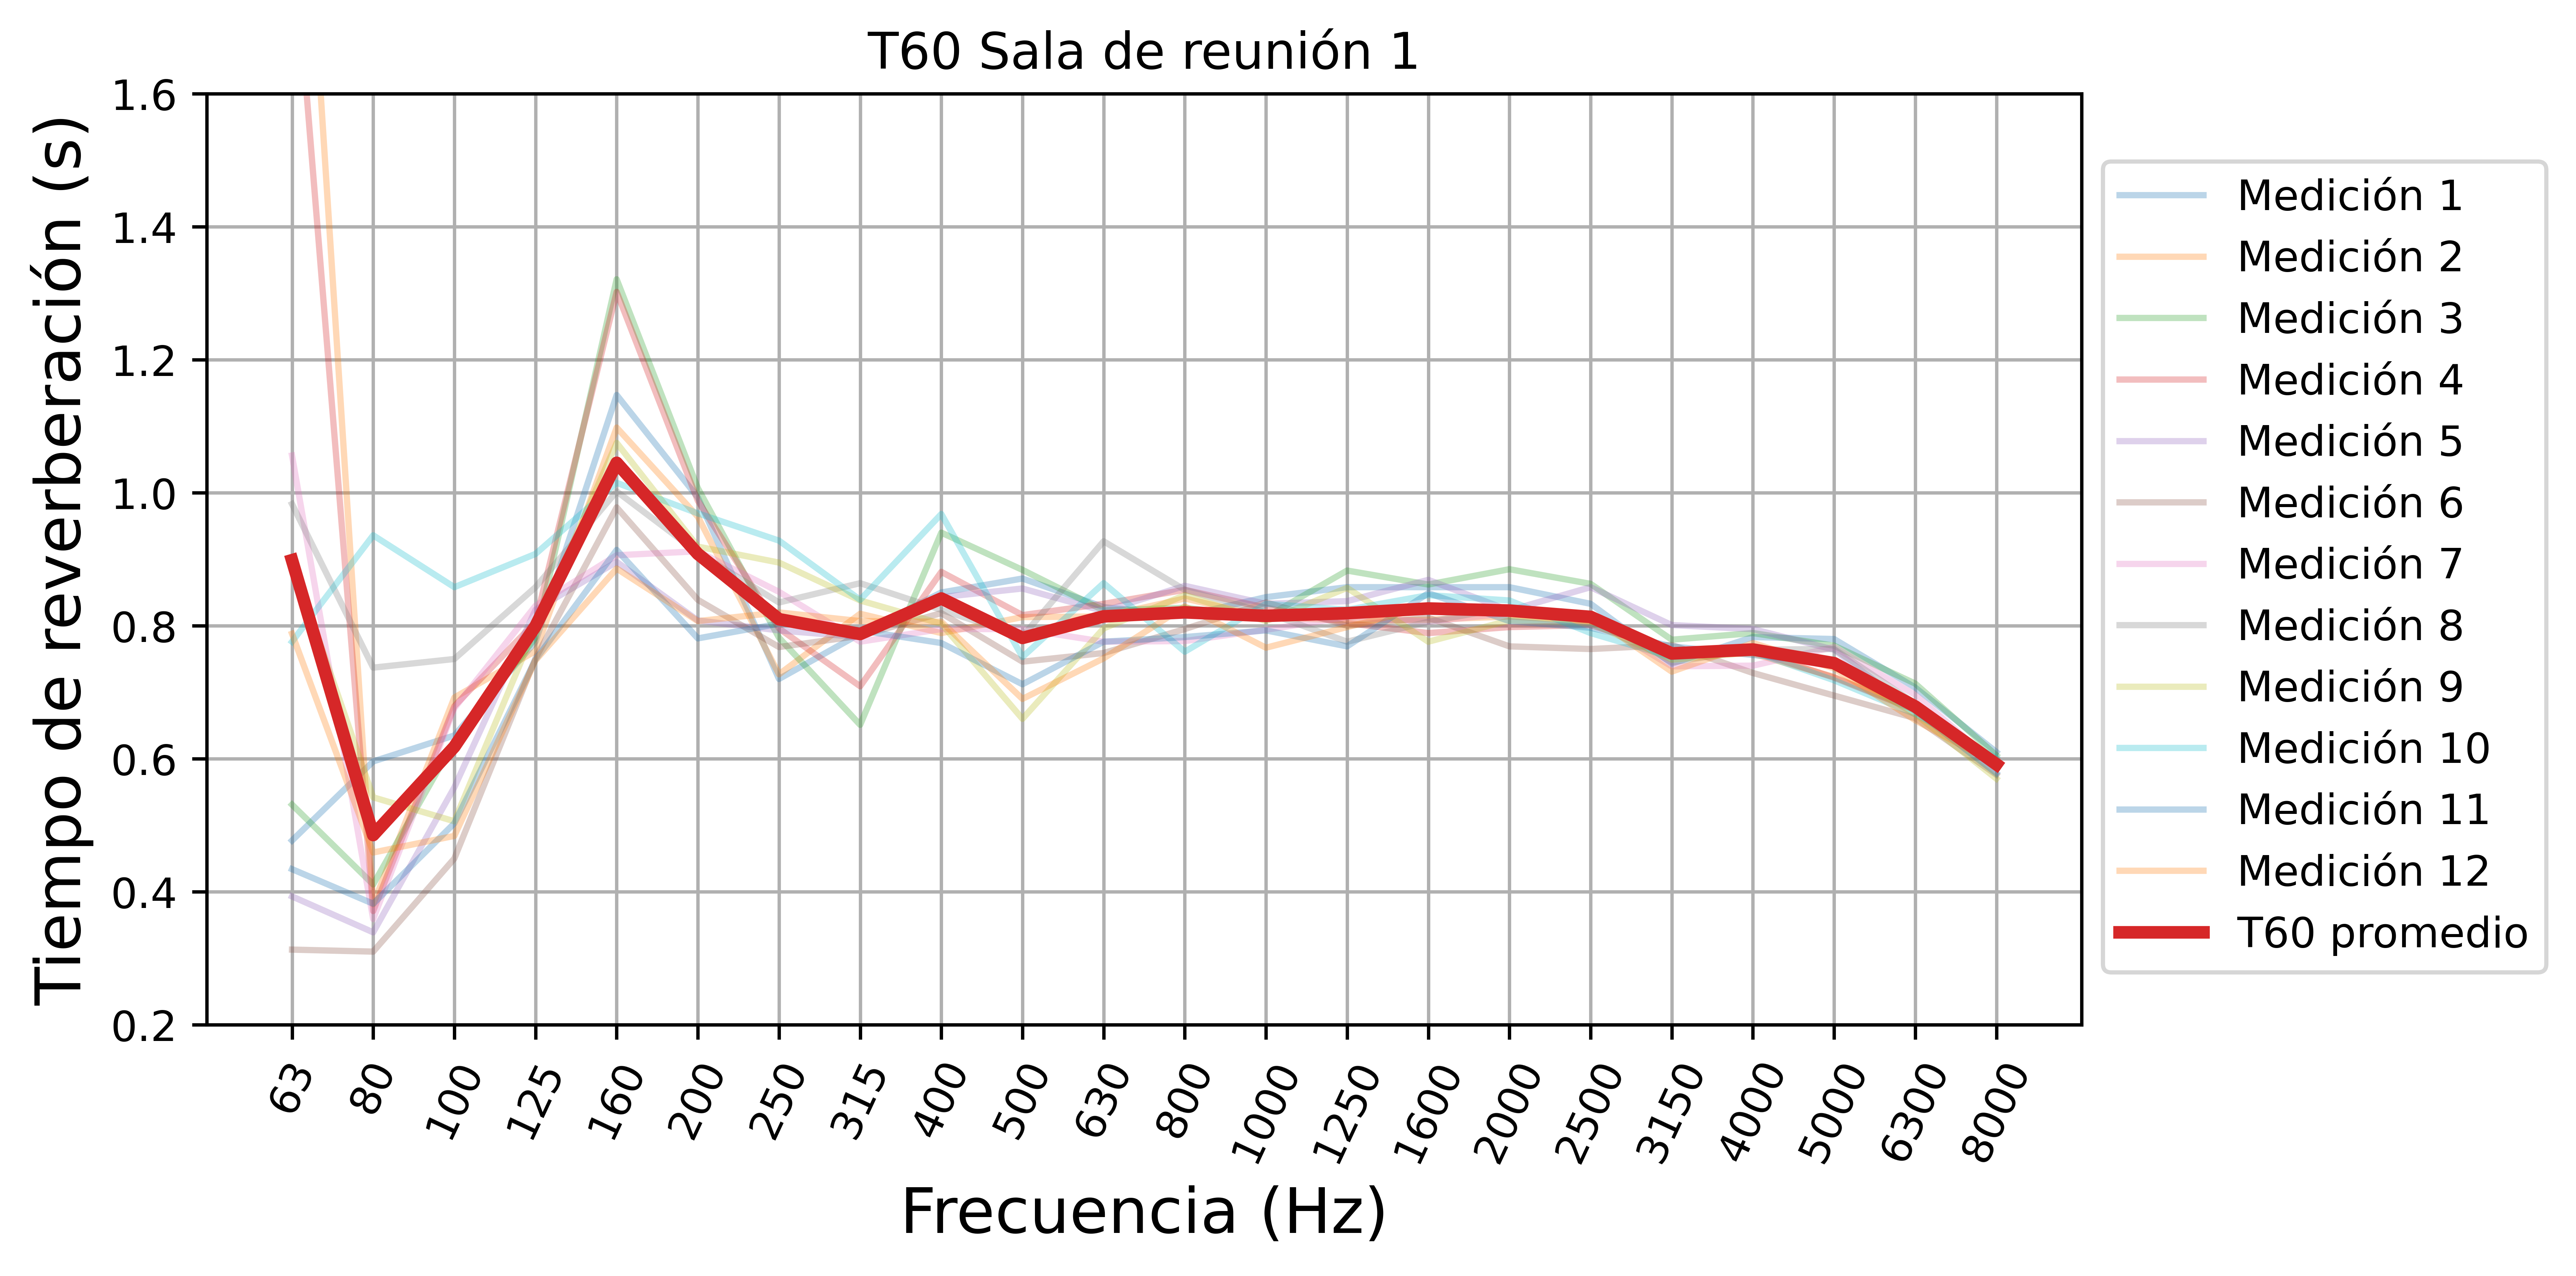
\includegraphics[width=12cm]{Imagenes/Resultados/T60_Sala_reunion_1.png}
    \caption{$T_{60}$ sala de reunión 1}
    \label{fig: T60 sala1}
\end{figure}

\begin{figure}[H]
    \centering
    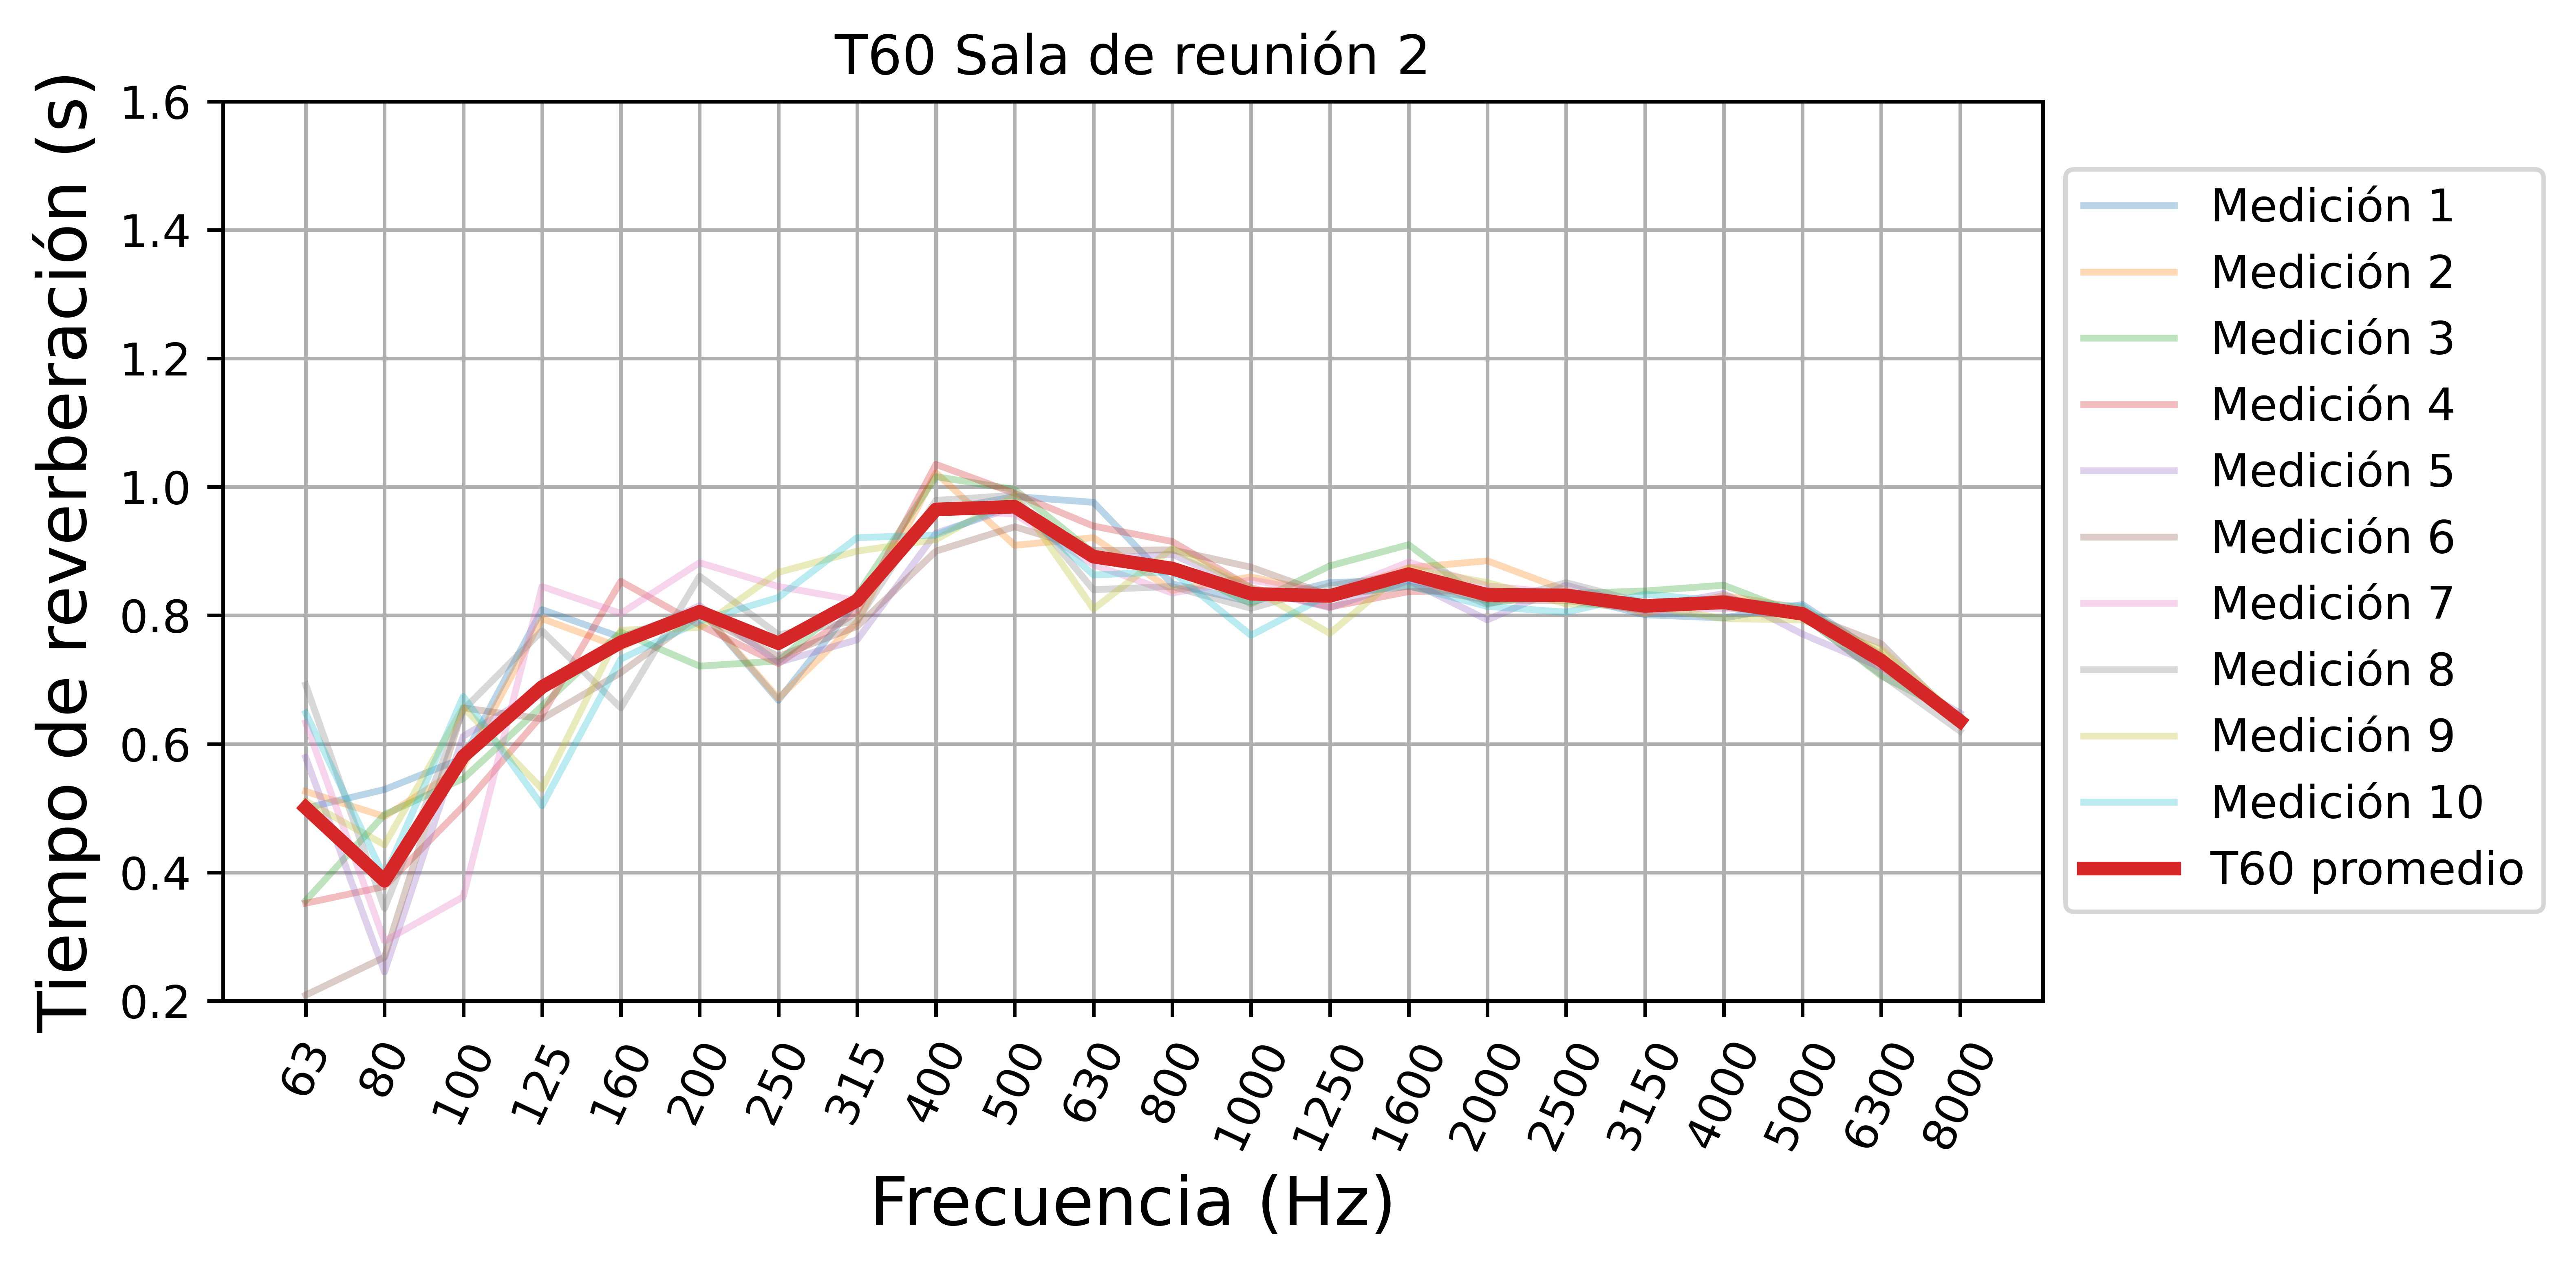
\includegraphics[width=12cm]{Imagenes/Resultados/T60_Sala_reunion_2.png}
    \caption{$T_{60}$ sala de reunión 2}
    \label{fig: T60 sala2}
\end{figure}

\begin{figure}[H]
    \centering
    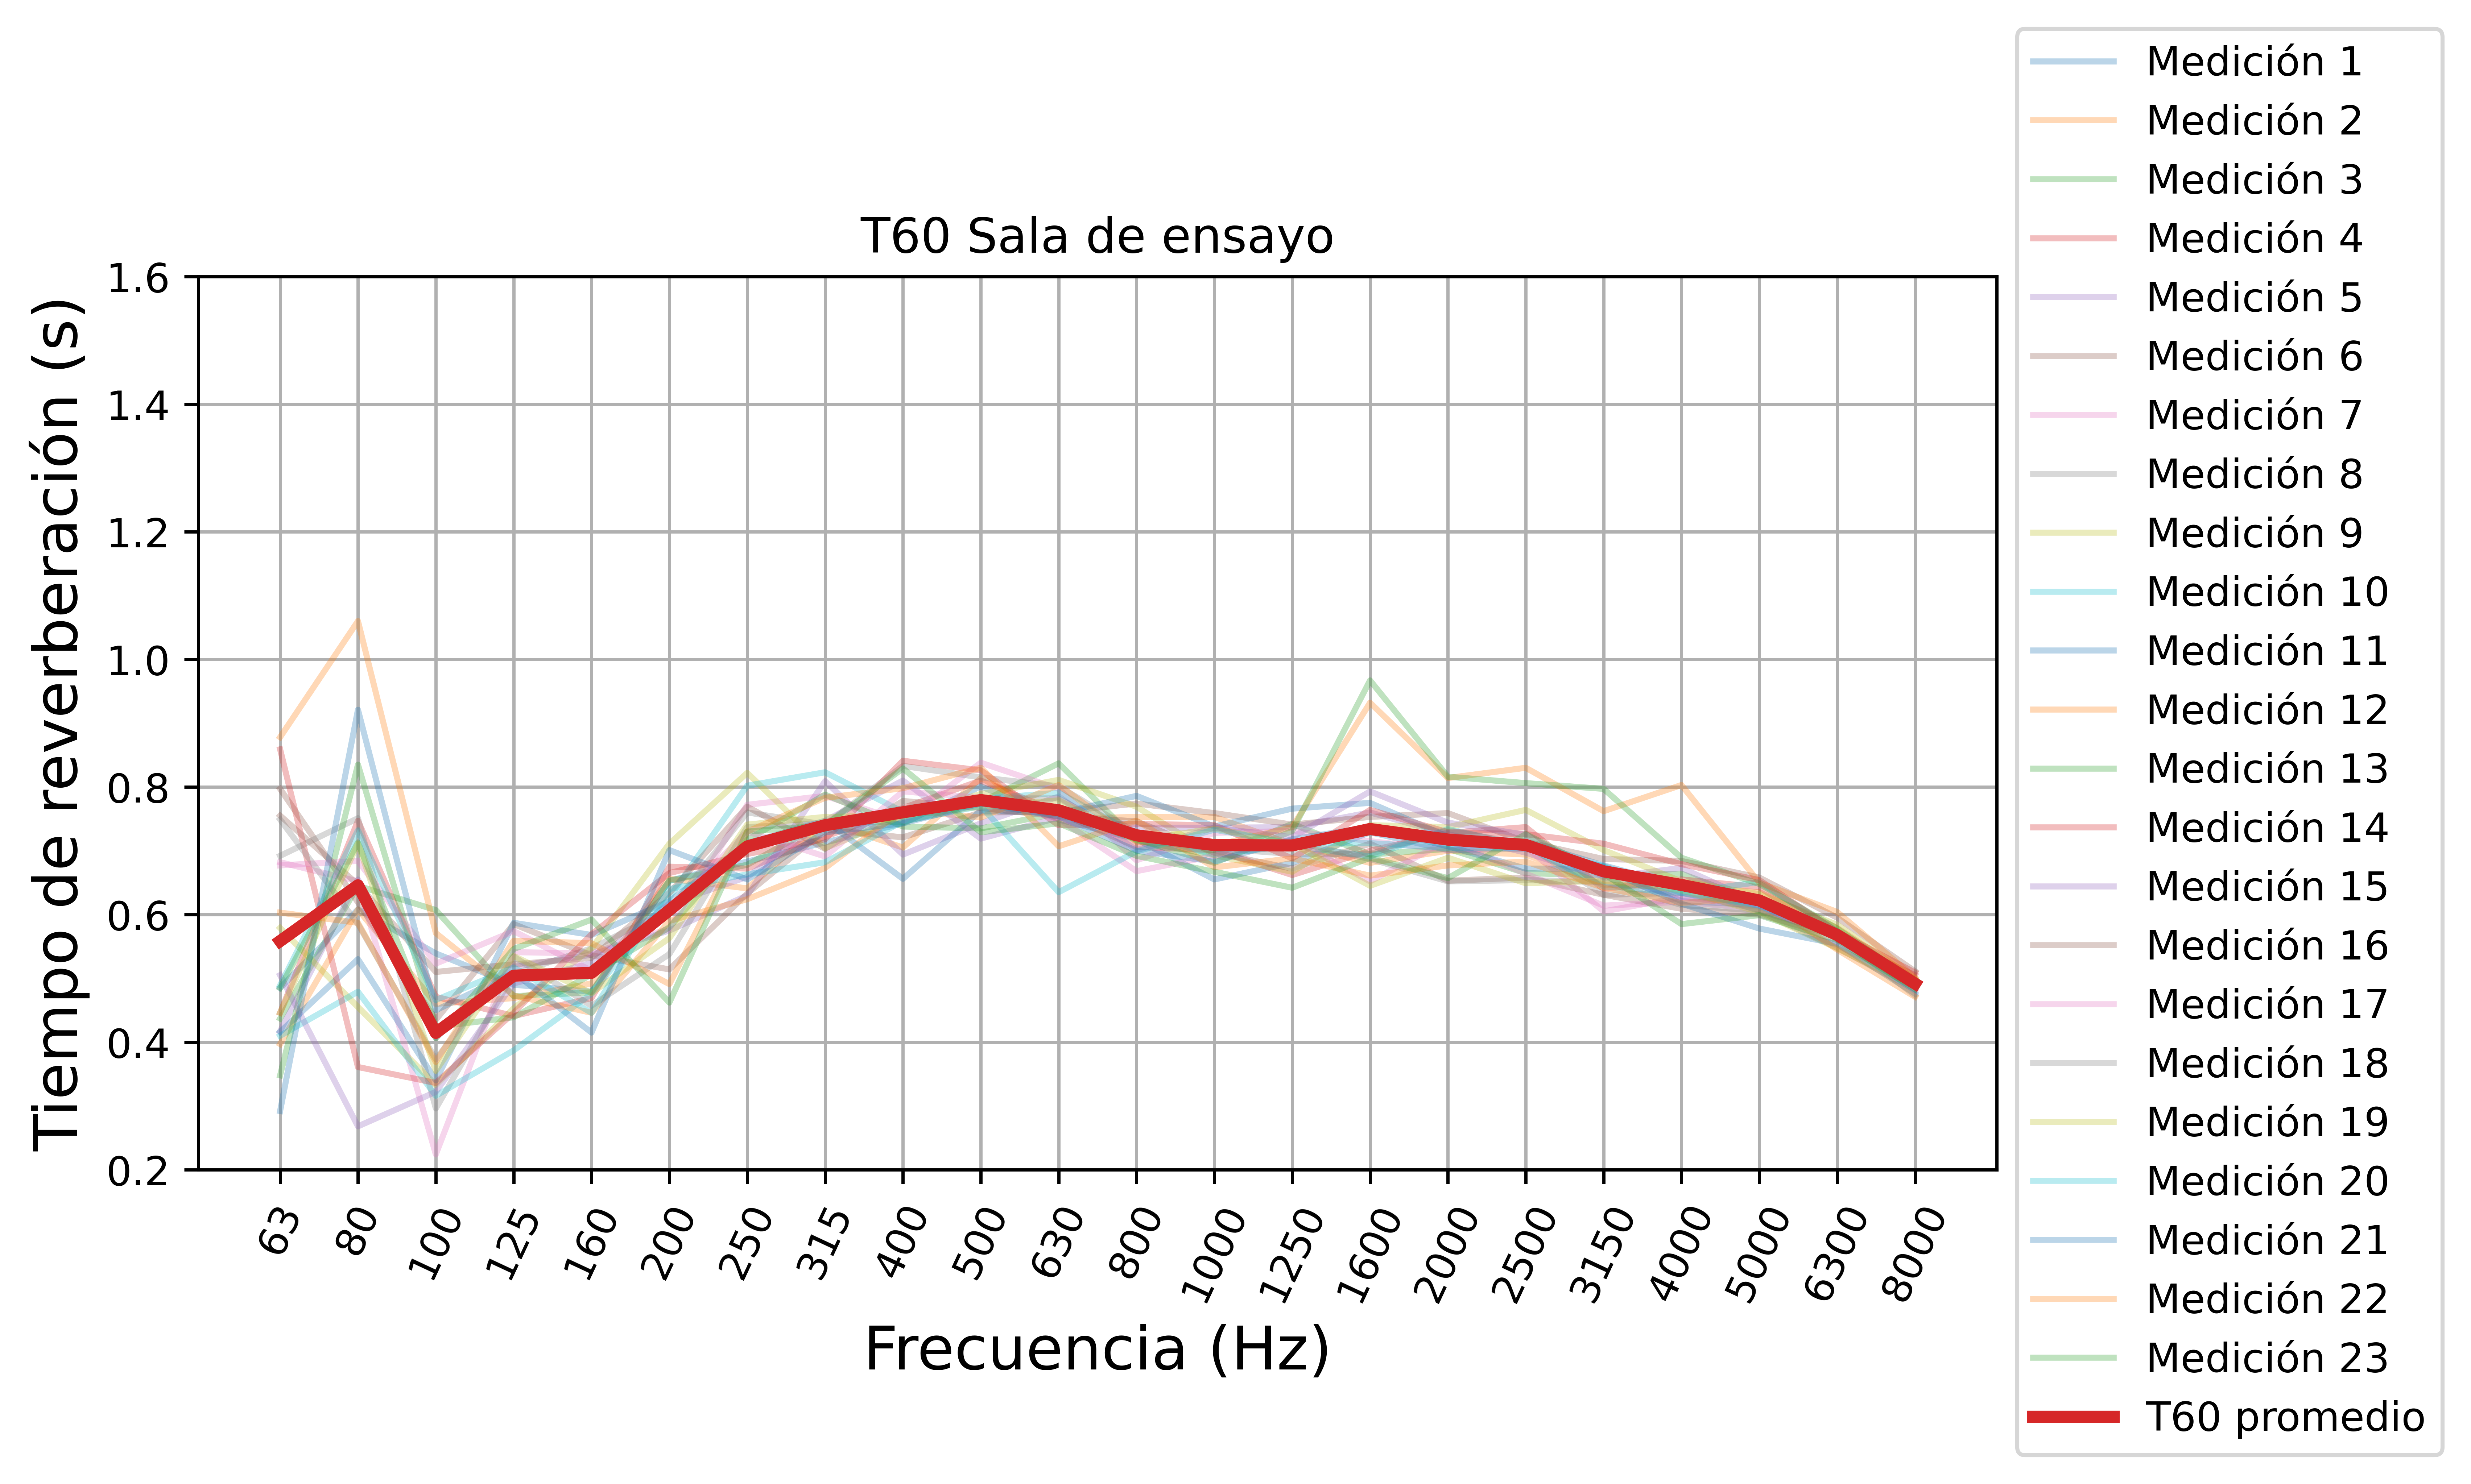
\includegraphics[width=12cm]{Imagenes/Resultados/T60_Sala_de_ensayo.png}
    \caption{$T_{60}$ sala de ensayo}
    \label{fig: T60 sala de ensayo}
\end{figure}

\subsection{STI actual}\label{subsecc: STI salas actual}
\begin{figure}[H]
    \centering
    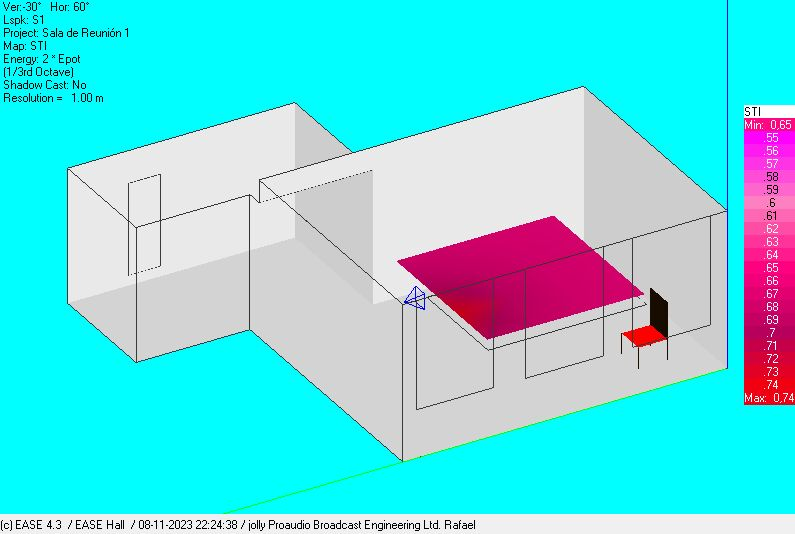
\includegraphics[width=12cm]{Imagenes/STI actual/STI_Reunion1_SinAcond.jpg}
    \caption{$STI$ actual de sala de reunión 1}
    \label{fig: STI sala1 actual}
\end{figure}
\begin{figure}[H]
    \centering
    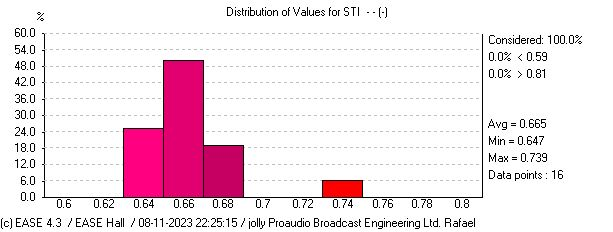
\includegraphics[width=12cm]{Imagenes/STI actual/STIdist_Reunion1_SinAcond.jpg}
    \caption{Distribución de $STI$ actual en sala de reunión 1}
    \label{fig: distribucion STI sala1 actual}
\end{figure}
\begin{figure}[H]
    \centering
    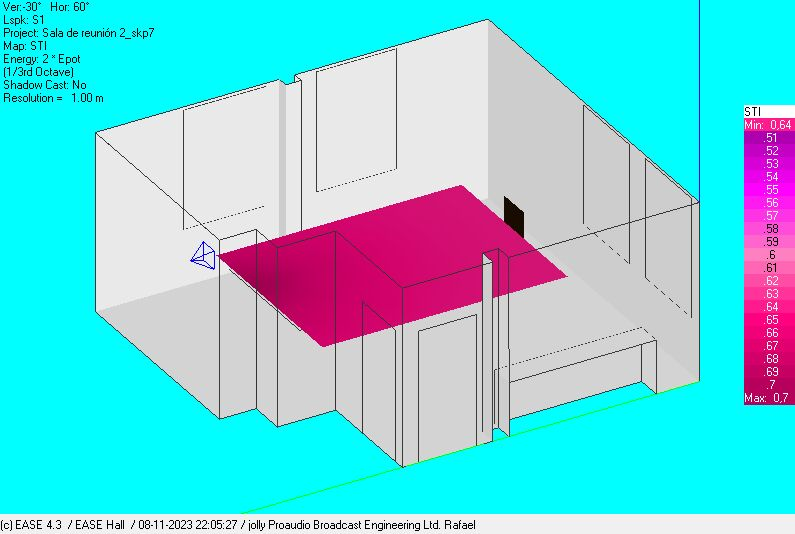
\includegraphics[width=12cm]{Imagenes/STI actual/STI_Reunion2_SinAcond.jpg}
    \caption{$STI$ actual de sala de reunión 2}
    \label{fig: STI sala2 actual}
\end{figure}
\begin{figure}[H]
    \centering
    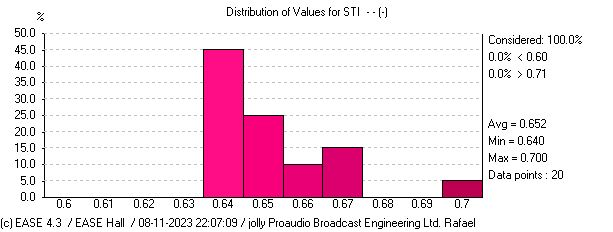
\includegraphics[width=12cm]{Imagenes/STI actual/STIdist_Reunion2_SinAcond.jpg}
    \caption{Distribución de $STI$ actual en sala de reunión 2}
    \label{fig: distribucion STI sala2 actual}
\end{figure}

\subsection{STI de salas de reunión acondicionadas}\label{subsecc: STI salas acond}
\begin{figure}[H]
    \centering
    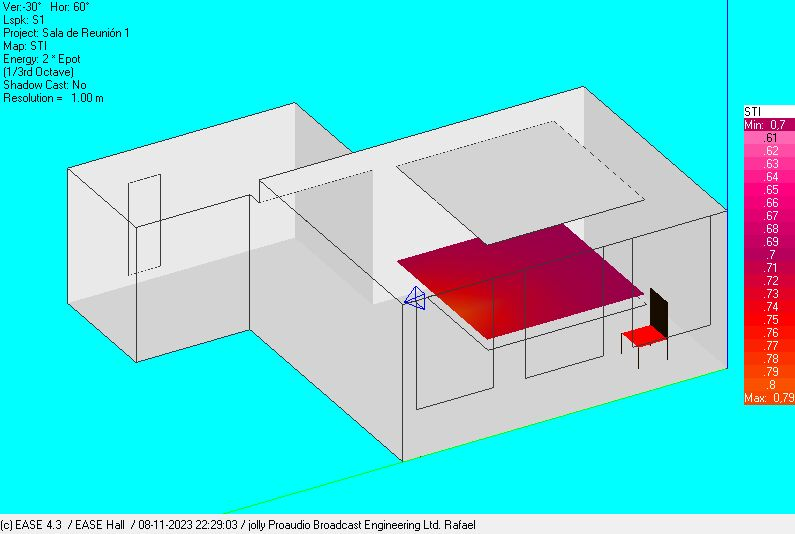
\includegraphics[width=12cm]{Imagenes/STI acondicionado/STI_Reunion1_ConAcond.jpg}
    \caption{$STI$ de sala de reunión 1 acondicionada}
    \label{fig: STI sala1 acond}
\end{figure}
\begin{figure}[H]
    \centering
    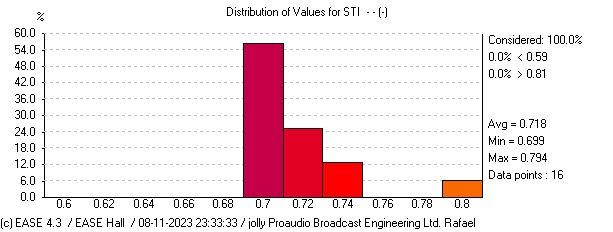
\includegraphics[width=12cm]{Imagenes/STI acondicionado/STIdist_Reunion1_ConAcond.jpg}
    \caption{Distribución de $STI$ en sala de reunión 1 acondicionada}
    \label{fig: distribucion STI sala1 acond}
\end{figure}

\begin{figure}[H]
    \centering
    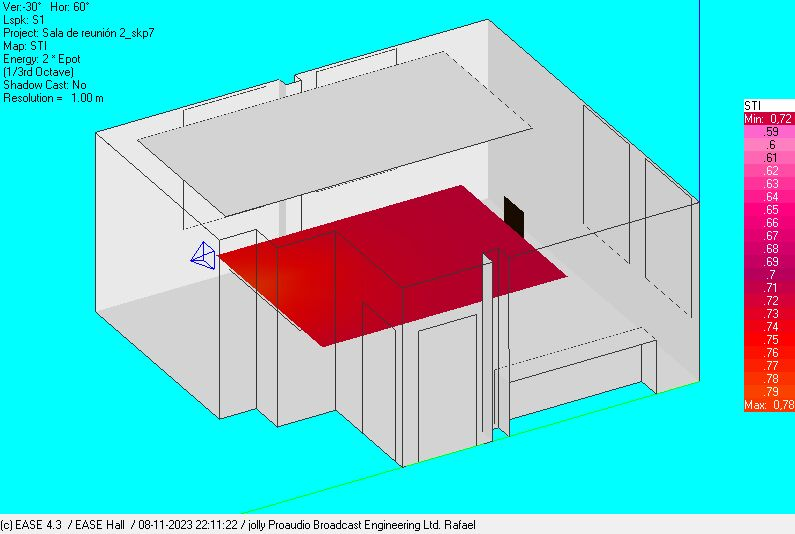
\includegraphics[width=12cm]{Imagenes/STI acondicionado/STI_Reunion2_ConAcond.jpg}
    \caption{$STI$ de sala de reunión 2 acondicionada}
    \label{fig: STI sala2 acond}
\end{figure}
\begin{figure}[H]
    \centering
    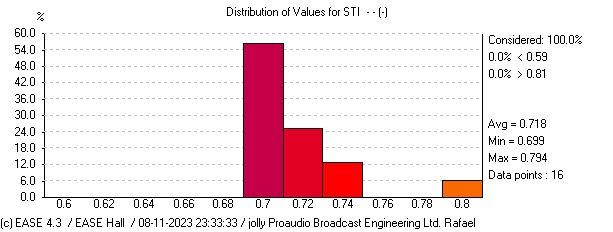
\includegraphics[width=12cm]{Imagenes/STI acondicionado/STIdist_Reunion1_ConAcond.jpg}
    \caption{Distribución de $STI$ en sala de reunión 2 acondicionada}
    \label{fig: distribucion STI sala2 acond}
\end{figure}
\end{document}